
\section{Introduction}

This appendix provides brief instructions to install the software packages that are used in this book. Most of the software is easy to install on both Windows and MacOS computers. However, websites, installation procedures, and the applications themselves may change over time. In case of problems, the reader should refer to the authoritative documentation for each software package.

\section{Installing Software on Windows}

\subsection{Installing R}

The R system for statistical computing can be downloaded from the Comprehensive R Archive Network (''CRAN''). CRAN is a repository of the R software itself as well as most of the libraries or packages. CRAN is distributed around the world, with different sites around the world offering the same content. This makes downloads faster.

\begin{resourcebox}
You can find the Comprehensive R Archive Network (''CRAN'') here:\\

\vspace{.5\baselineskip}
\url{htts://cran.r-project.org}
\end{resourcebox}

\clearpage
\begin{itemize}
\item On the CRAN website, navigate to the download page for Windows. Select the latest ''base'' version of R to download. At the time of writing, this was version 4.5.2.

\begin{center}
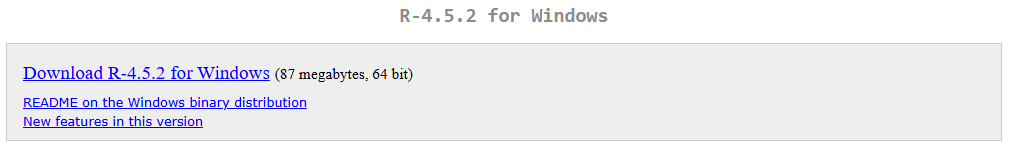
\includegraphics[width=.95\textwidth]{Rscreen1.png}
\end{center}

\item Once the download is complete, open and run the downloaded installer file. 

\begin{center}
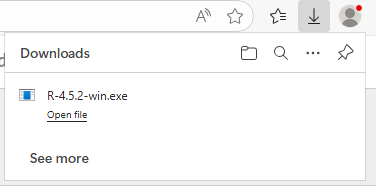
\includegraphics[width=.55\textwidth]{Rscreen2.png}
\end{center}

\item Once the installer finished, click the ''Finish'' button.

\begin{center}
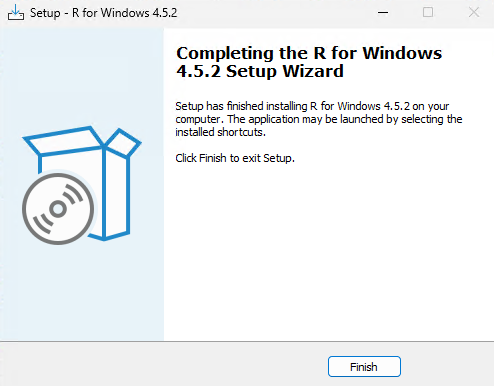
\includegraphics[width=.65\textwidth]{Rscreen3.png}
\end{center}

\clearpage
\item Launch the R software from the Windows Start menu.

\begin{center}
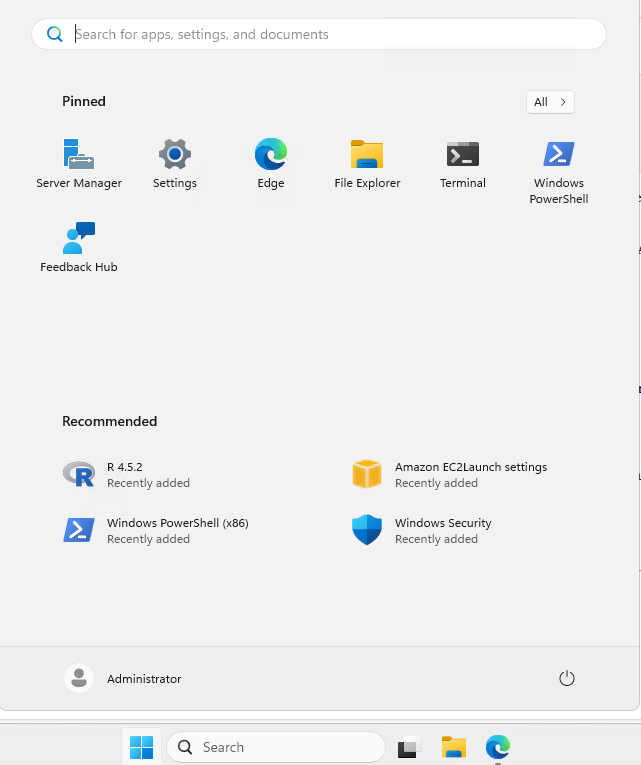
\includegraphics[width=.55\textwidth]{Rscreen4.png}
\end{center}

\item You will see the R graphical user interface. You can enlarge the inner window titled ''R Console'' using the button in the top right corner of its window frame.

\begin{center}
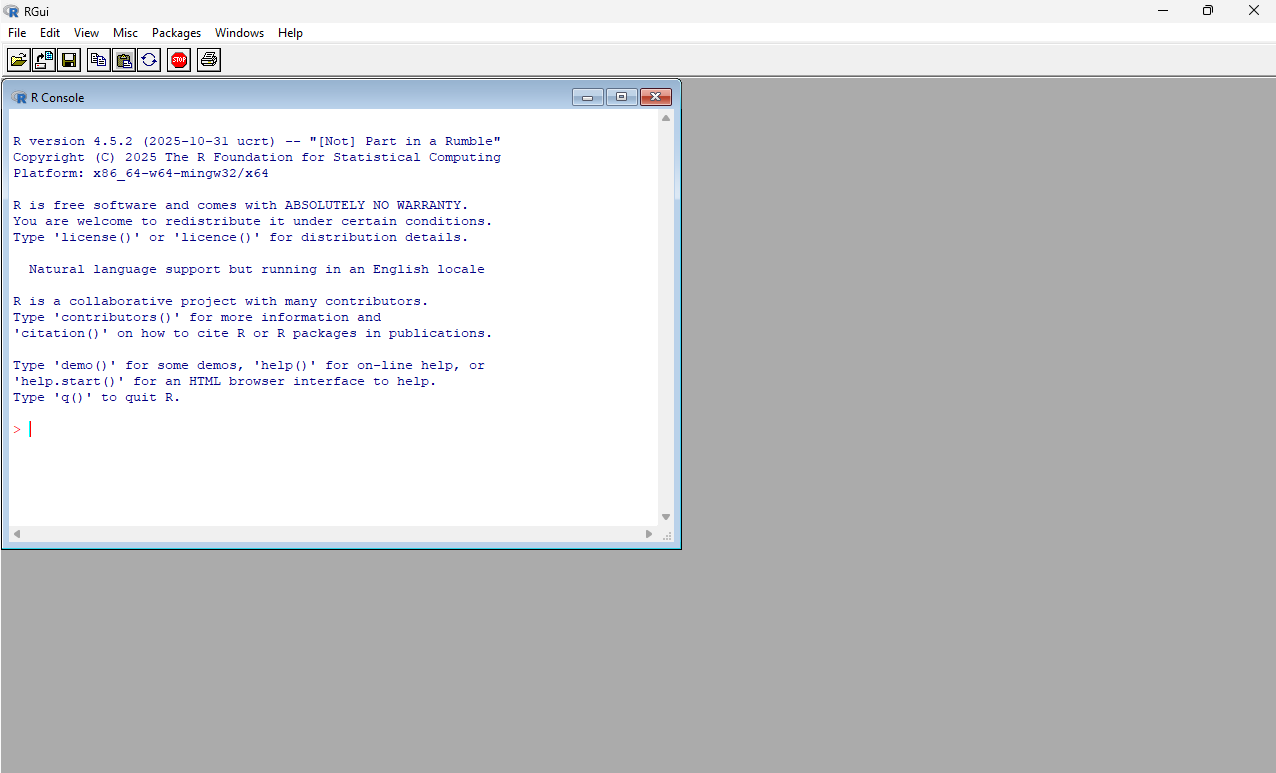
\includegraphics[width=.85\textwidth]{Rscreen5.png}
\end{center}

\clearpage
\item Copy and paste the following R command into the R window. Then, hit the enter key on your keyboard to execute it. This command will install the R packages used in this book.

\begin{Rcode}
install.packages(c('tidyverse', 'boot', 'zoo', 'astsa', 
'devtools', 'fGarch', 'ggpattern', 'scales', 'ISLR2', 
'class', 'glmnet', 'e1071', 'ROCR', 'sqldf', 'ggsci'))
\end{Rcode}

\begin{center}
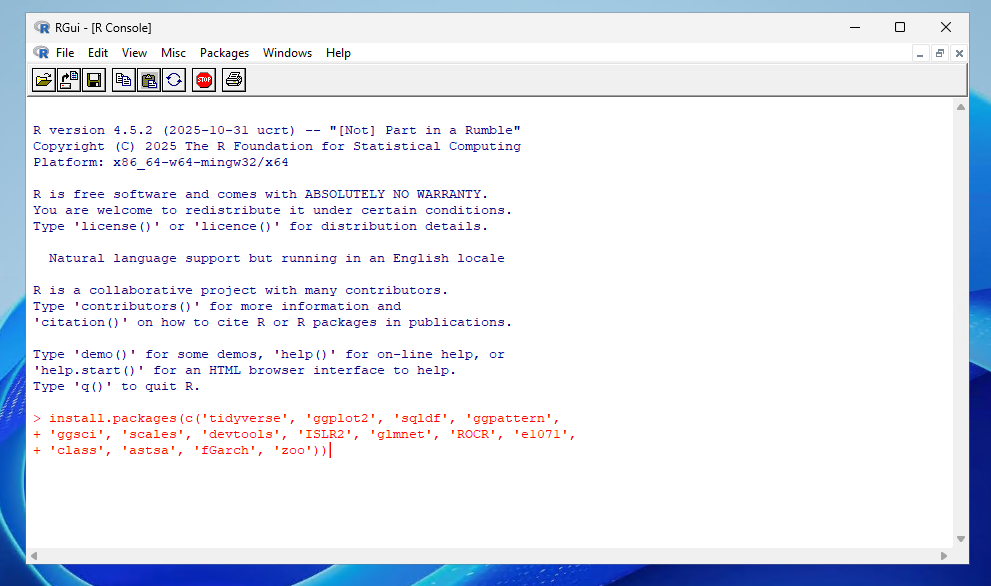
\includegraphics[width=.85\textwidth]{Rscreen6.png}
\end{center}

You will be asked whether you wish to create a personal library for these packages and you will be given a default location for this library. Click ''Yes'' on both questions.

\clearpage
You may be asked to choose a CRAN mirror. The software on all mirrors is identical but choosing one that is geographically close greatly improves the download speed.

\begin{center}
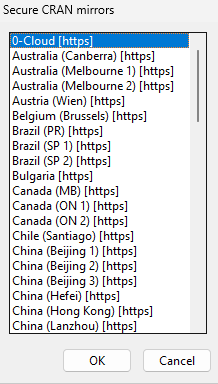
\includegraphics[width=.35\textwidth]{Rscreen7.png}
\end{center}

\item You can quit R by executing the following command in the R window or simply by closing the R window itself.

\begin{Rcode}
quit()
\end{Rcode}

\end{itemize}

\begin{infobox}
The downloaded versions of the R libraries may be newer than those used for the writing of this book. While it is not expected that their behaviour will change, you may wish to consult the libraries' manuals if it does.
\end{infobox}

\clearpage
\subsection{Installing Python using WSL}

The easiest way to use Python on Windows is through the use of the WSL2, the Windows Subsystem for Linux. This allows running the latest version of all packages without the difficulties or peculiarities of Windows. To install and configure WSL follow these instructions.

\begin{itemize}

\item On your Windows computer, open the Start menu, then find the ''PowerShell for Windows''. Right-click on it and select ''Run in Administrator'' or select it in the Start menu and then click on ''Run in Administrator''.

\begin{center}

\includegraphics[width=.65\textwidth]{screen1.png}
\end{center}

\item Type the command ''wsl --install'' into the PowerShell window and hit the enter key on your keyboard to execute this command.

\begin{center}

\includegraphics[width=.85\textwidth]{screen2.png}
\end{center}

Once complete, you can close the PowerShell window.

\item Restart your computer.

\item Start PowerShell and type the command ''wsl --install Ubuntu'' in the PowerShell window and hit the enter key on your keyboard to execute this command.

\begin{center}

\includegraphics[width=.85\textwidth]{screen3.png}
\end{center}

\item You will be asked to create a user account. By default, WSL will use your Windows login name but you may change this. You will also be asked to enter a new password. Do not forget this password.

\begin{center}

\includegraphics[width=.85\textwidth]{screen4.png}
\end{center}

\begin{center}

\includegraphics[width=.85\textwidth]{screen5.png}
\end{center}

\item Type ''exit'' to close the application, then close the PowerShell window.

\begin{center}

\includegraphics[width=.85\textwidth]{screen6.png}
\end{center}

\item To use WSL and the chosen Linux distribution (''Ubuntu''), choose either ''WSL'' or ''Ubuntu'' from your Windows Start menu.

\begin{center}

\includegraphics[width=.55\textwidth]{screen7.png}
\end{center}

\clearpage
\item You will see the WSL Ubuntu command window.

\begin{center}

\includegraphics[width=.85\textwidth]{screen8.png}
\end{center}

\item Copy and paste the following commands into this window and hit the enter key on your keyboard to execute them. You will be asked to enter the password you created earlier. Type ''Y'' for yes if asked to confirm your actions. These commands will update the packages and then install some Python components.

\begin{bashcode}
sudo apt update
sudo apt upgrade
sudo apt install python-is-python3 python3-pip python3-venv
\end{bashcode}

\item Copy and paste the following commands into this window and hit the enter key on your keyboard to execute them. This will set up a Python virtual environment to install the required Python packages into.

\begin{bashcode}
python -m venv venv
source venv/bin/activate
\end{bashcode}

\item Copy and paste the following command into this window and hit the enter key on your keyboard to execute it. This will install all Python packages used in this book and the packages they in turn depend on.

\begin{bashcode}
pip install -r https://www.evermann.ca/busi4720/requirements.txt
\end{bashcode}

\clearpage
Downloading and installing all packages will take a few minutes. You should see a success message similar to the following screenshot.

\begin{center}

\includegraphics[width=.85\textwidth]{screen14.png}
\end{center}

\item Deactivate the Python virtual environment using the following command:

\begin{bashcode}
deactivate
\end{bashcode}

\begin{alertbox}
To use Python, you will need to 
\begin{enumerate}
\item Start WSL or Ubuntu from the Windows Start menu
\item Activate the Python virtual environment with the following command
\begin{bashcode}
source venv/bin/activate
\end{bashcode}
\item Start Python with the following command
\begin{bashcode}
python
\end{bashcode}
\item To exit Python, enter the following Python command
\begin{pythoncode}
quit()
\end{pythoncode}
\item Close the WSL/Ubuntu window
\end{enumerate}
\end{alertbox}

\begin{infobox}
The downloaded versions of the Python packages may be newer than those used for the writing of this book. While it is not expected that their behaviour will change, you may wish to consult the packages' manuals if it does.
\end{infobox}

\end{itemize}

\clearpage
\subsection{Installing PostgreSQL}

\begin{resourcebox}
PostgreSQL is available for Windows and MacOS systems and installation applications can be found via its website. \\

\url{https://www.postgresql.org}
\end{resourcebox}

\begin{itemize}
\item Navigate to the Downloads section of the PostgreSQL website. Then select the Windows installer.

\begin{center}
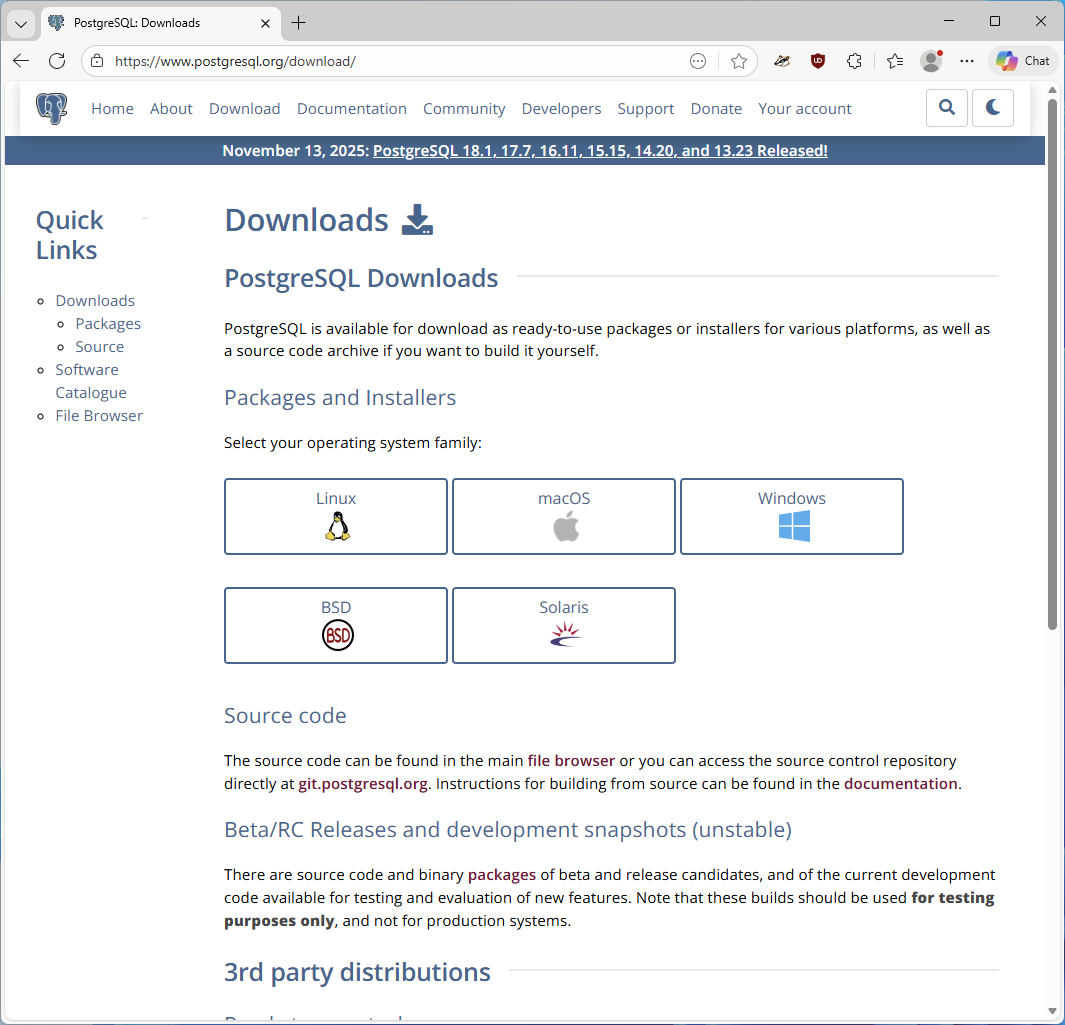
\includegraphics[width=.75\textwidth]{screen15.png}
\end{center}

\clearpage
\item Select the Windows downloader for the latest version of PostgreSQL.

\begin{center}
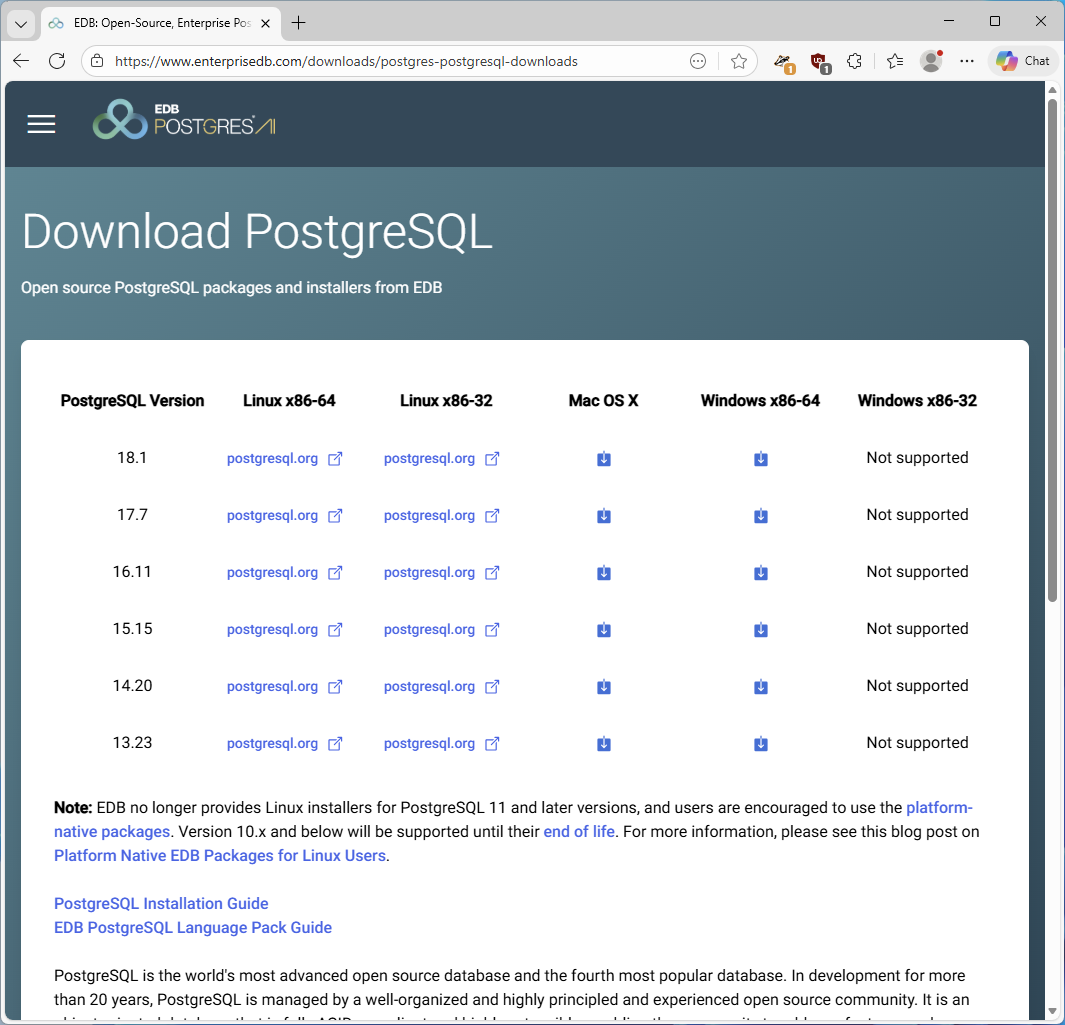
\includegraphics[width=.75\textwidth]{screen16.png}
\end{center}

\item Once the download is completed, open the downloaded file.

\begin{center}
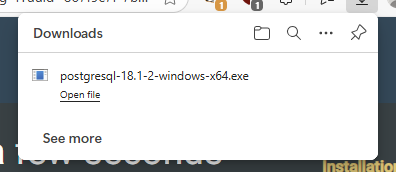
\includegraphics[width=.55\textwidth]{screen17.png}
\end{center}

\item Two required software packages may be automatically installed before the PostgreSQL installer is shown.

\clearpage
\item Click the ''Next'' button on each installer dialog window. You do not need to change any of the values or options.

\begin{center}
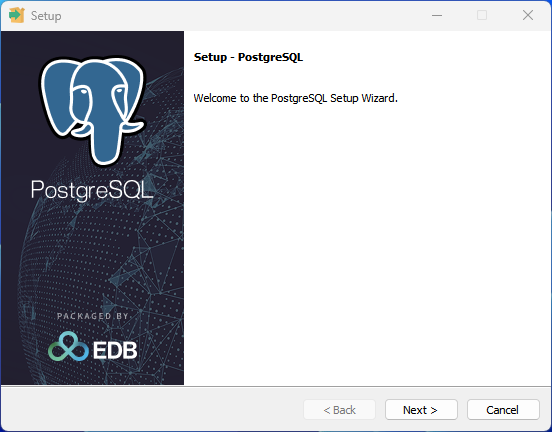
\includegraphics[width=.65\textwidth]{screen18.png}
\end{center}

\item You will be asked to enter a password for the super user of the database system. Enter a password that you will remember, as you will need it later.

\begin{center}
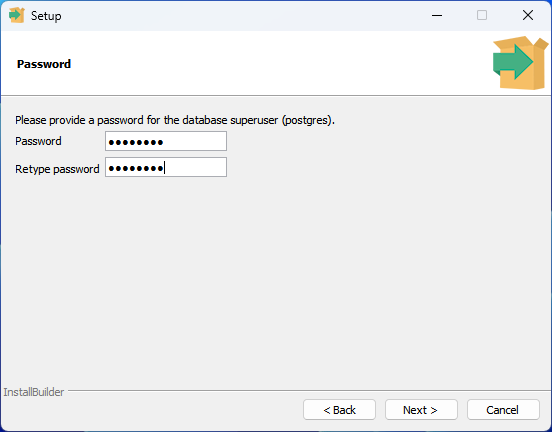
\includegraphics[width=.65\textwidth]{screen19.png}
\end{center}

Continue with the installation by clicking the ''Next'' button on each installer dialog window.

\clearpage
\item Once the installation is finished, you do need to launch Stack Builder. Unselect the tick box, then click the ''Finish'' button.

\begin{center}
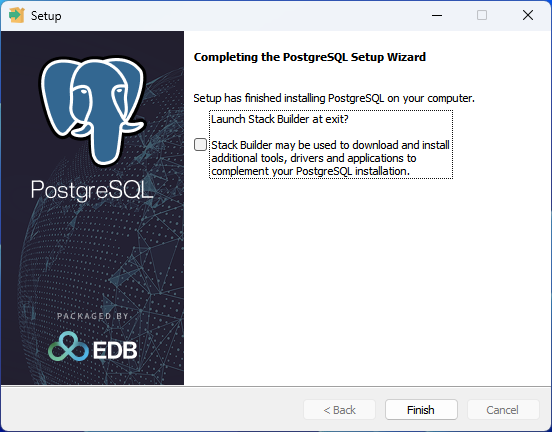
\includegraphics[width=.65\textwidth]{screen20.png}
\end{center}

\item Once the installation is complete, select the PostgreSQL 18 section from the Windows Start menu and launch the pgAdmin4 application.

\begin{center}
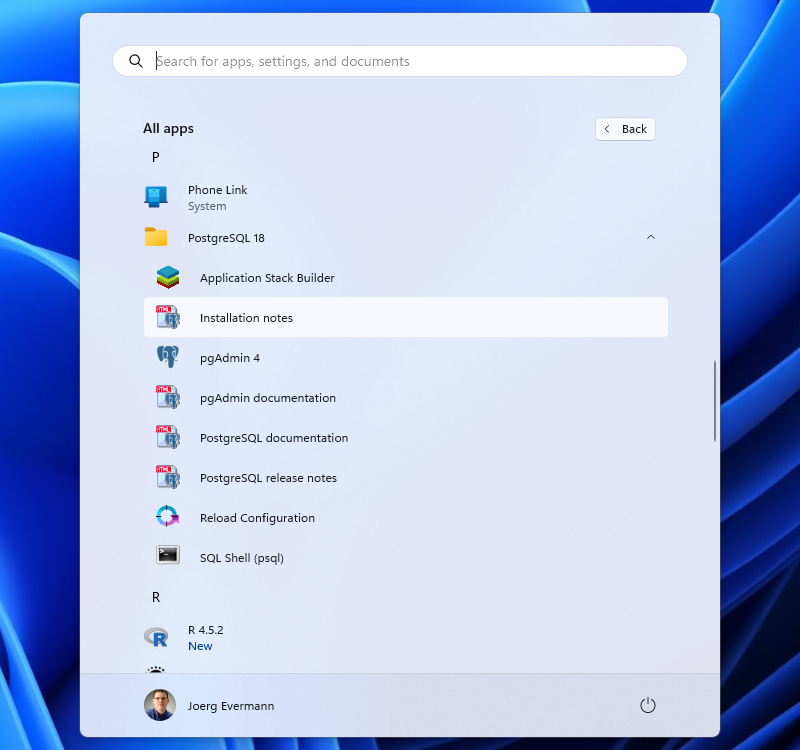
\includegraphics[width=.65\textwidth]{screen21.png}
\end{center}

\clearpage
\item You will be asked to enter the password for the user ''postgres'' that you chose earlier. 

\begin{center}
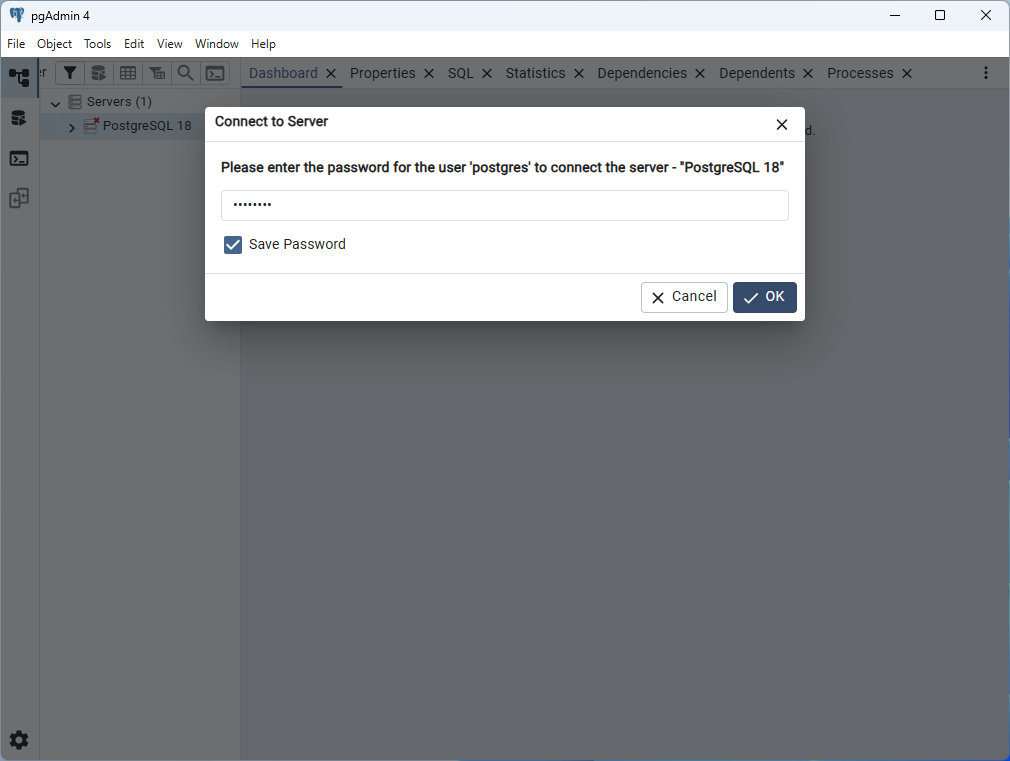
\includegraphics[width=.85\textwidth]{screen22.png}
\end{center}

\item Once logged in, you will see the pgAdmin dashboard view.

\begin{center}
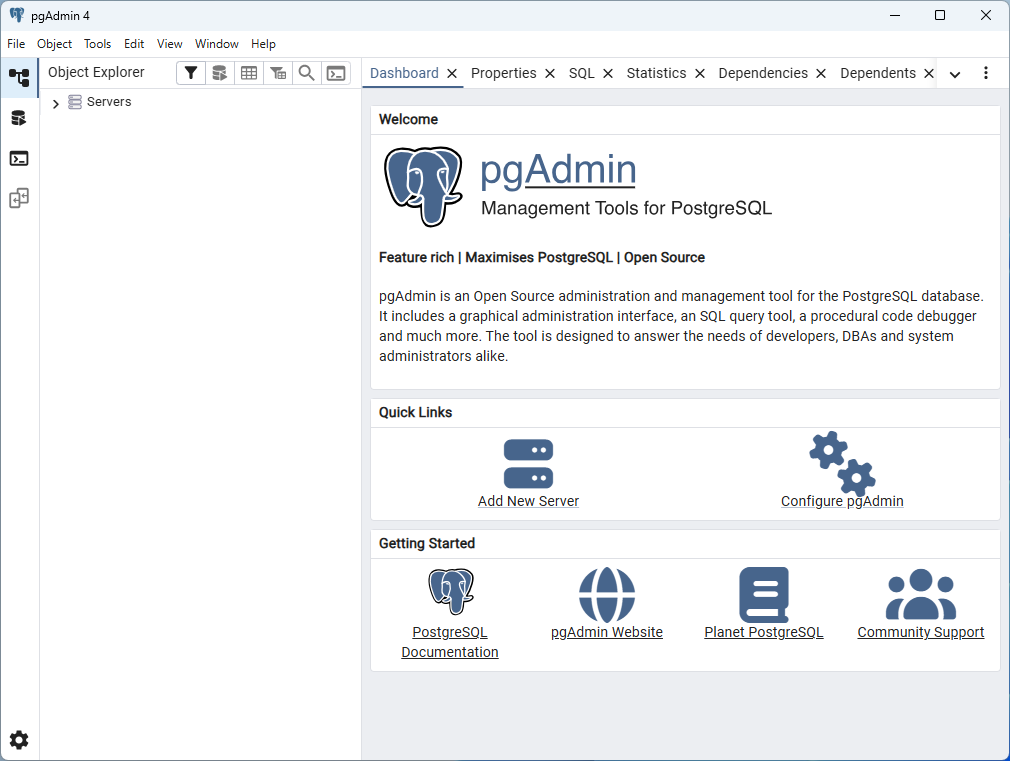
\includegraphics[width=.85\textwidth]{screen23.png}
\end{center}

\clearpage
\item In the ''Object Explorer'' on the left, navigate to the ''postgres'' database.

\begin{center}
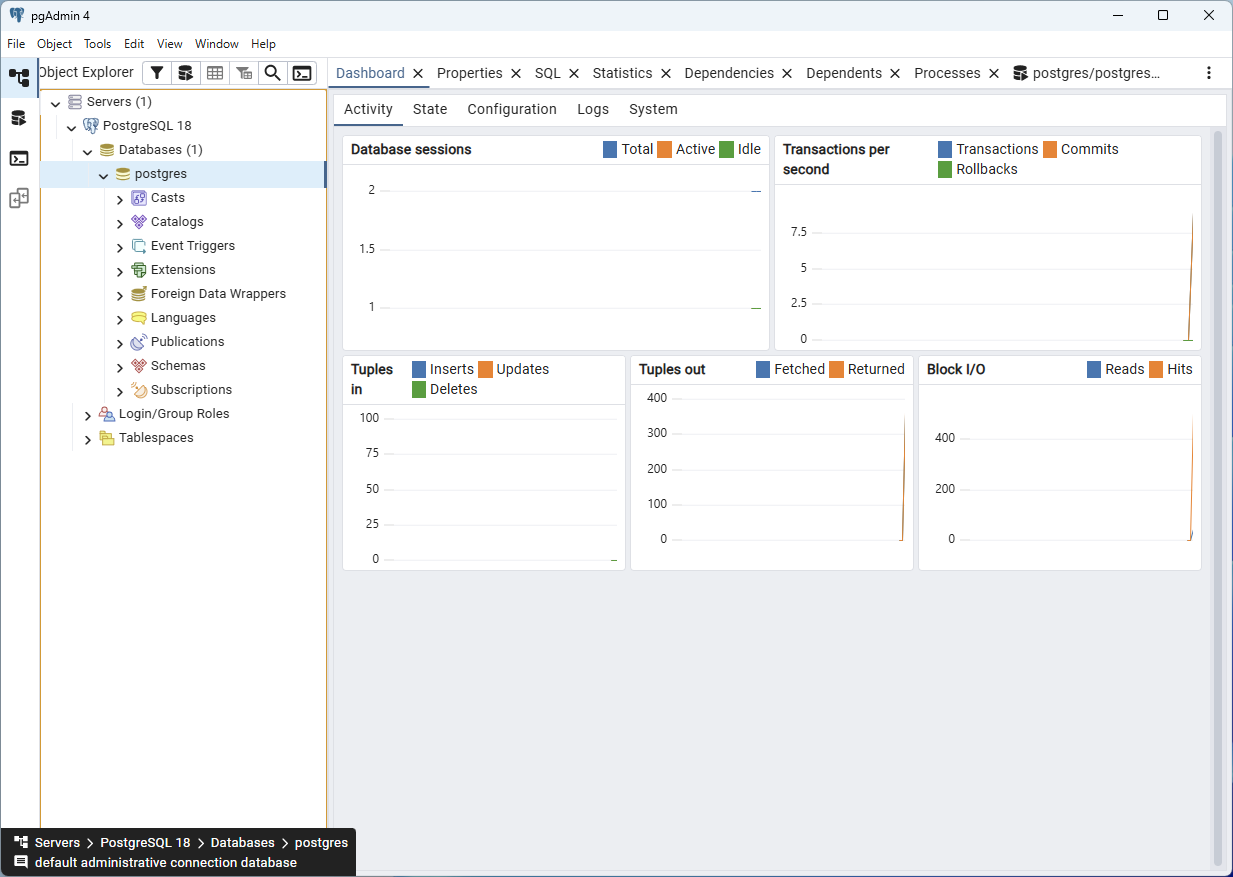
\includegraphics[width=.85\textwidth]{screen24.png}
\end{center}

\begin{resourcebox}
The \emph{Pagila} database is a demonstration database designed to illustrate database concepts. \\

\url{https://github.com/devrimgunduz/pagila} \\

To install the ''Pagila'' demo database, download the following two files and save them to your computer. 

\begin{enumerate}
\item \url{https://www.evermann.ca/busi4720/pagila-schema.sql}
\item \url{https://www.evermann.ca/busi4720/pagila-insert-data.sql}
\end{enumerate}
\end{resourcebox}

\clearpage
\item In the pgAdmin application, choose ''Query Tool'' from the main menu.

\begin{center}
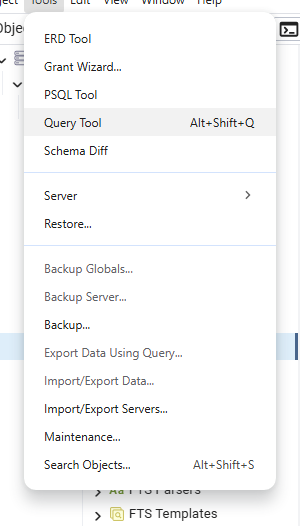
\includegraphics[width=.35\textwidth]{screen25.png}
\end{center}

You will be shown a new Query Tool window in the pgAdmin application.

\begin{center}
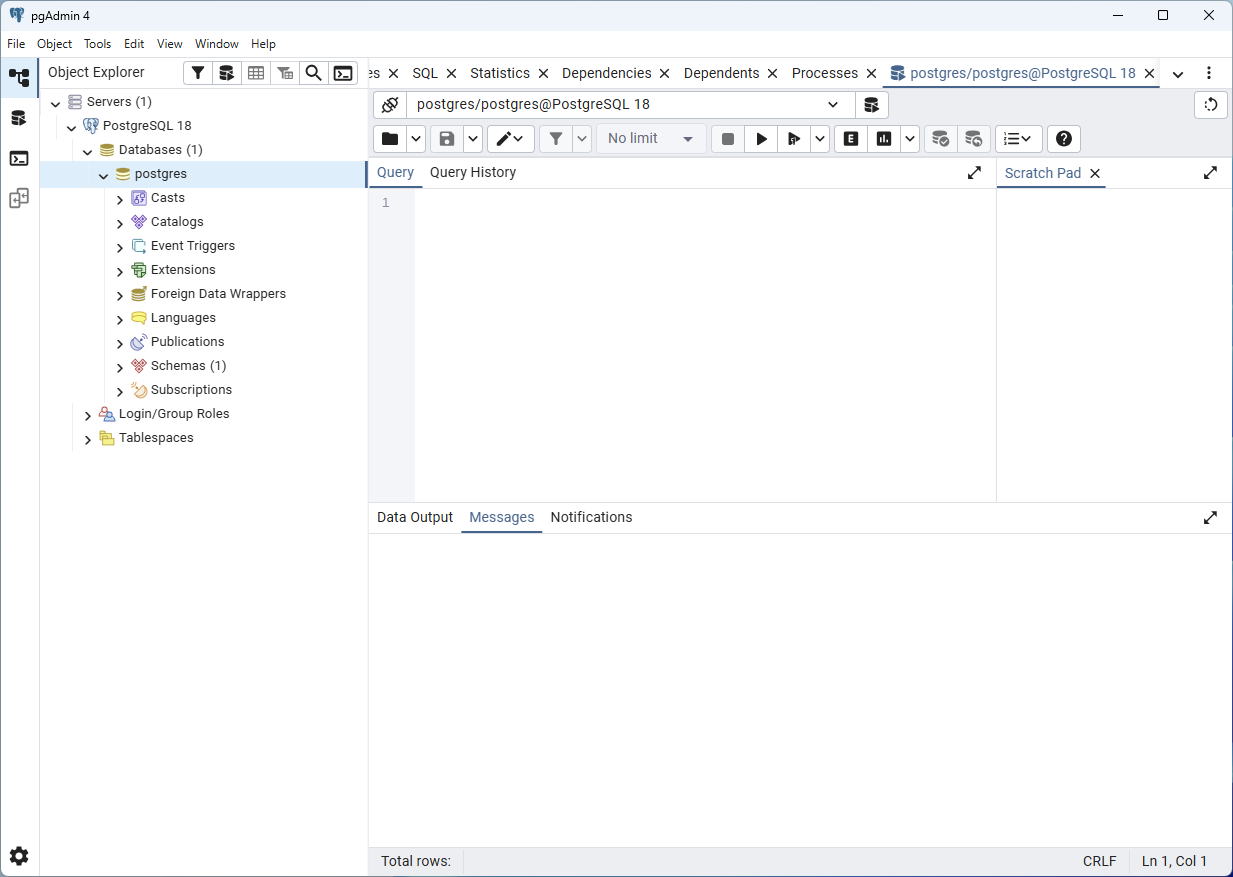
\includegraphics[width=.85\textwidth]{screen25a.png}
\end{center}

\clearpage
\item In the Query Tool, click the ''Open File'' button.

\begin{center}
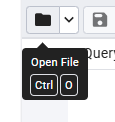
\includegraphics[width=.25\textwidth]{screen26.png}
\end{center}

\item Find and open the downloaded file ''pagila-schema.sql'' 

\begin{center}
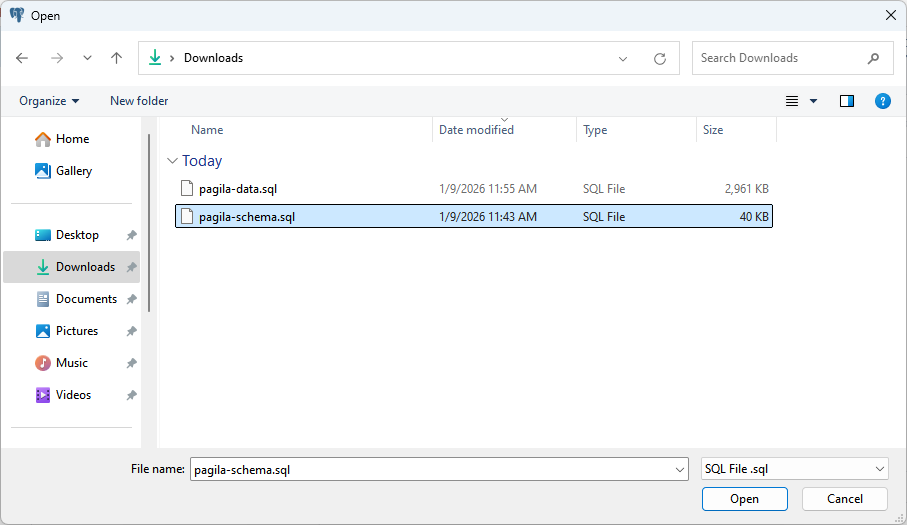
\includegraphics[width=.85\textwidth]{screen27.png}
\end{center}

\item In the Query Tool, click the ''Execute Script'' button.

\begin{center}
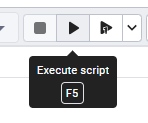
\includegraphics[width=.25\textwidth]{screen28.png}
\end{center}

\item In the pgAdmin application, choose ''Query Tool'' from the main again. Repeat the above three steps for the file ''pagila-insert-data.sql''

You have now installed the Pagila database.

\end{itemize}

\subsection{Installing Neo4J}

\begin{resourcebox}
Neo4J is a graph database that is available for Windows and MacOS systems. There are different ways to install it but the easiest is to use the Neo4J for Desktop version that is intended for database developers. The installation application for this Neo4J version can be found via its website. \\

\url{https://www.neo4j.com/download/}
\end{resourcebox}

\begin{itemize}

\item Navigate to the Neo4J for Desktop download page and click the ''Download'' button.

\begin{center}
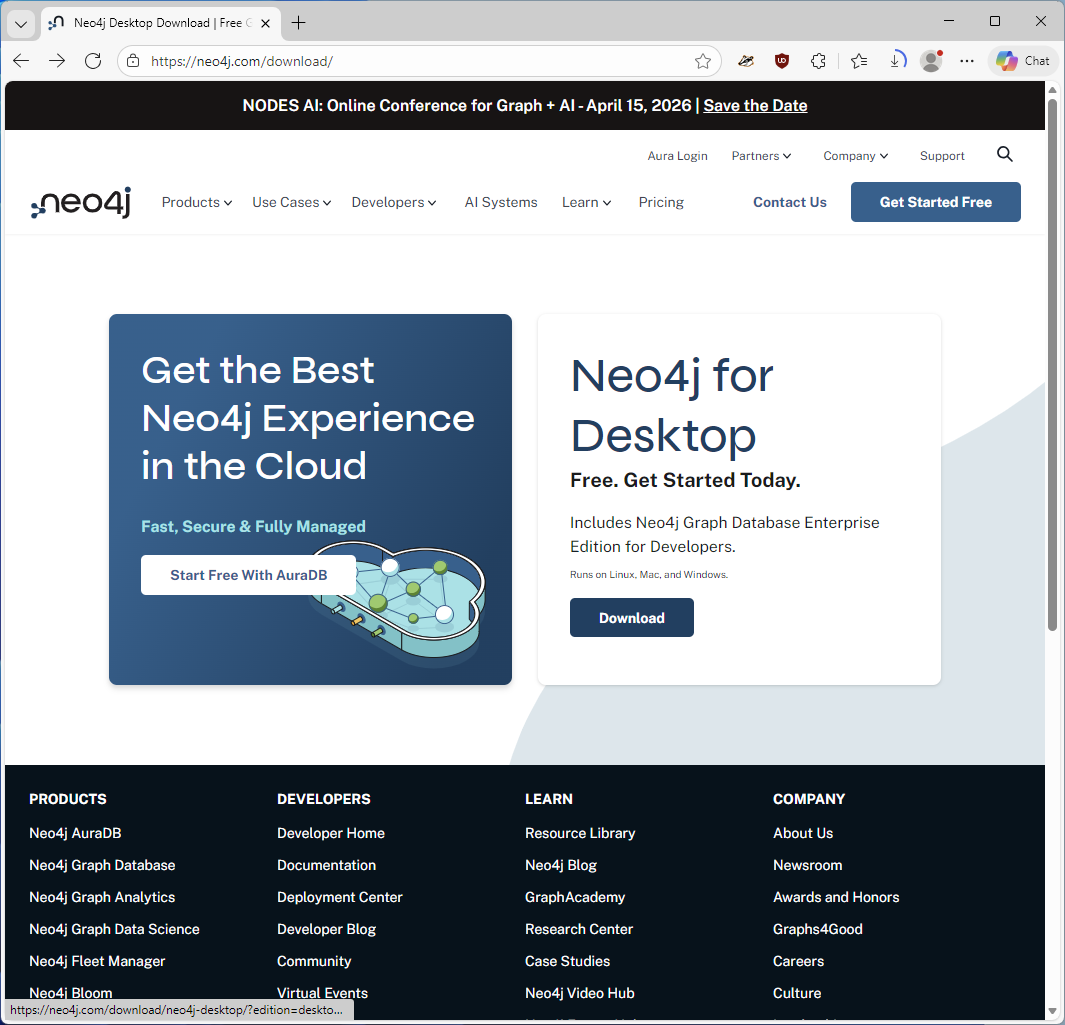
\includegraphics[width=.85\textwidth]{screen29.png}
\end{center}

\clearpage
\item After the download, you may receive a warning by your Edge web browser that the application may not be safe.

\begin{center}
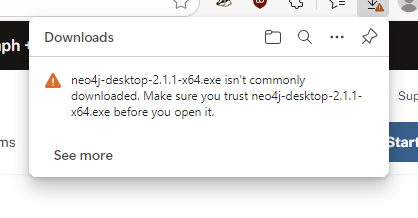
\includegraphics[width=.55\textwidth]{screen30.png}
\end{center}

Click on the warning, then select the ellipsis (''...'') next to the ''Delete'' button, then select ''Keep anyway''

\begin{center}
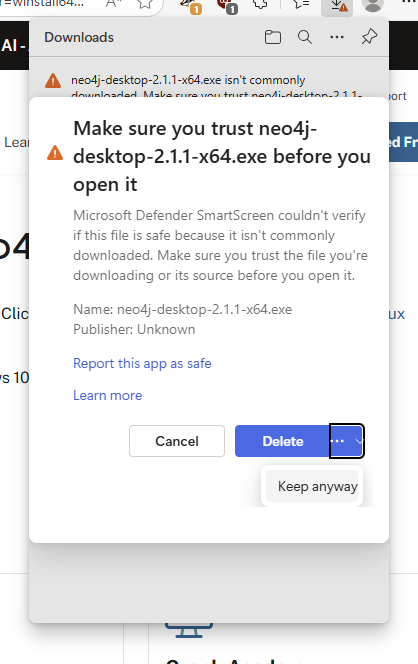
\includegraphics[width=.55\textwidth]{screen31.png}
\end{center}

\clearpage
\item Open the downloaded file to install Neo4J for Desktop.

\begin{center}
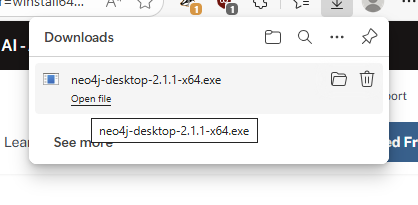
\includegraphics[width=.55\textwidth]{screen32.png}
\end{center}

Installing the application may take a few minutes.

\begin{center}
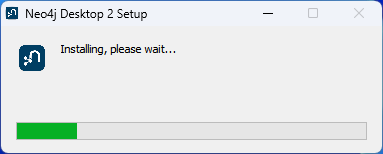
\includegraphics[width=.55\textwidth]{screen33.png}
\end{center}

\item When asked whether to allow networks to access this app, select ''Yes''.

\begin{center}
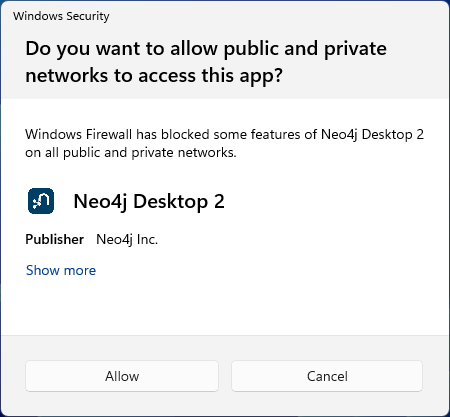
\includegraphics[width=.45\textwidth]{screen34.png}
\end{center}

\clearpage
\item The Neo4J application will start and present you with a license agreement which you must accept by clicking the ''Continue'' button.

\begin{center}
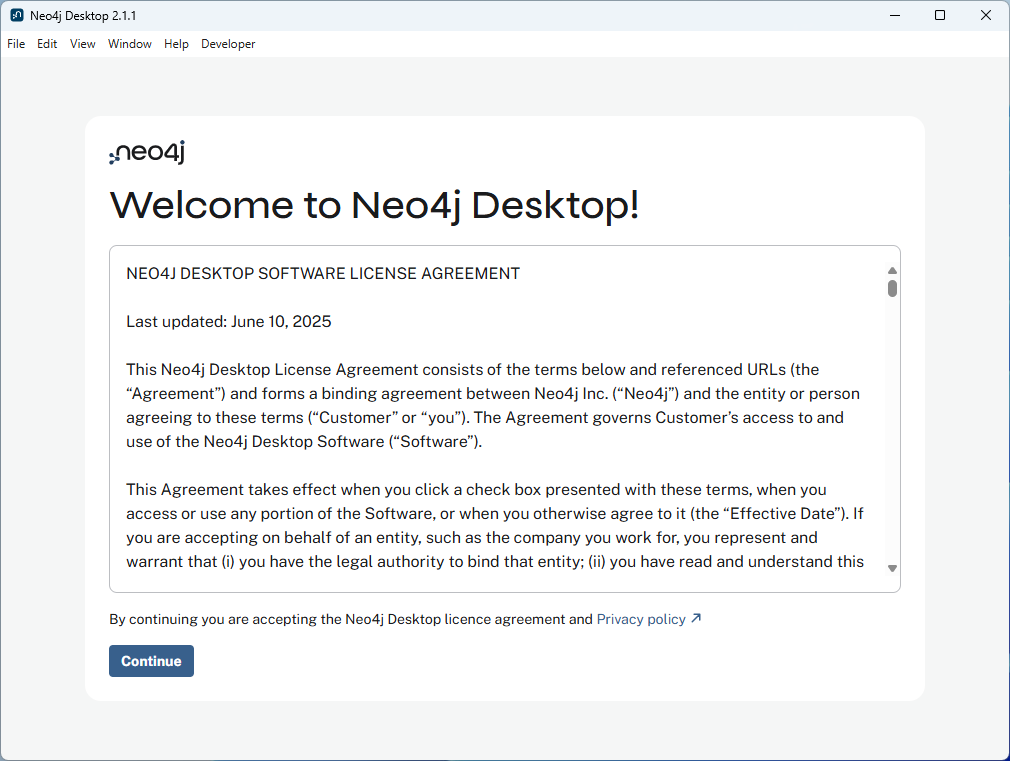
\includegraphics[width=.85\textwidth]{screen35.png}
\end{center}

\item Neo4J will ask you create a database server instance and a database in that. Click the ''Create instance'' button.

\begin{center}
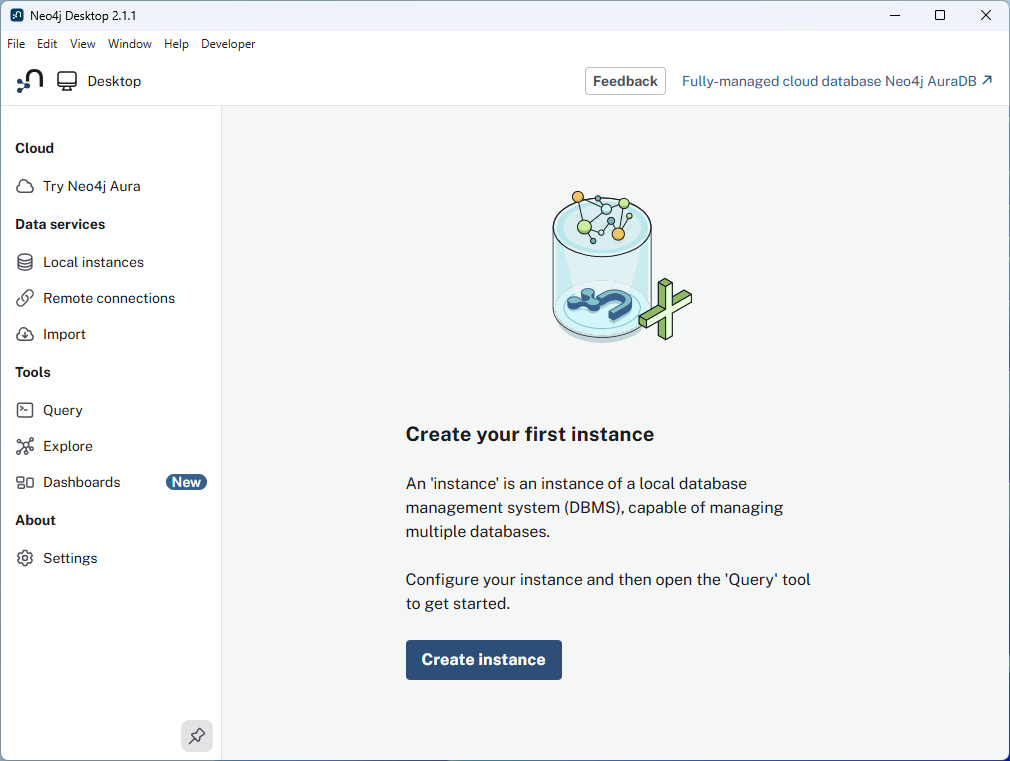
\includegraphics[width=.85\textwidth]{screen36.png}
\end{center}

\clearpage
\item Give the instance a name of your choice, e.g. ''busi4720'' and provide a new password for the database user. Select the option to load from .dump, .backup or .tar file.

\begin{center}
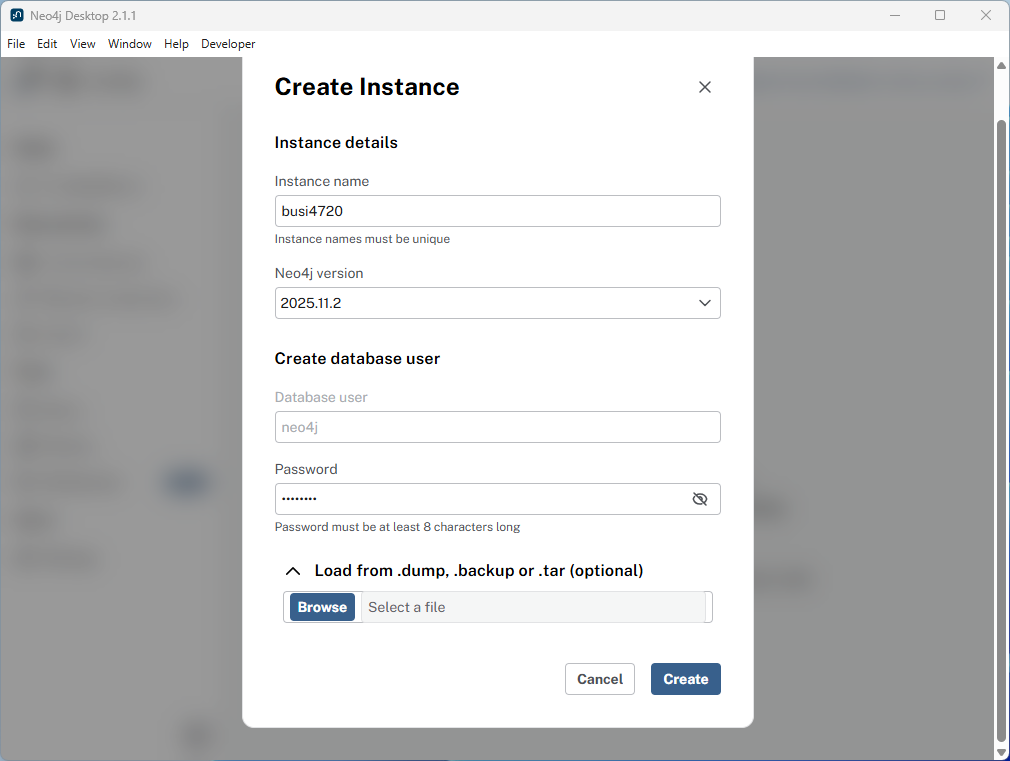
\includegraphics[width=.85\textwidth]{screen37.png}
\end{center}

\begin{resourcebox}
The \emph{Pagila} database is a demonstration database designed to illustrate database concepts. A version of Pagila for Neo4J is available for download. \\

Download and save the following file to your computer.

\begin{enumerate}
\item \url{https://www.evermann.ca/busi4720/neo4j_db_pagila.dump}
\end{enumerate}
\end{resourcebox}

\item Next, in the Neo4J application, select the ''Browse'' button and find and open the file you just downloaded.

\begin{center}
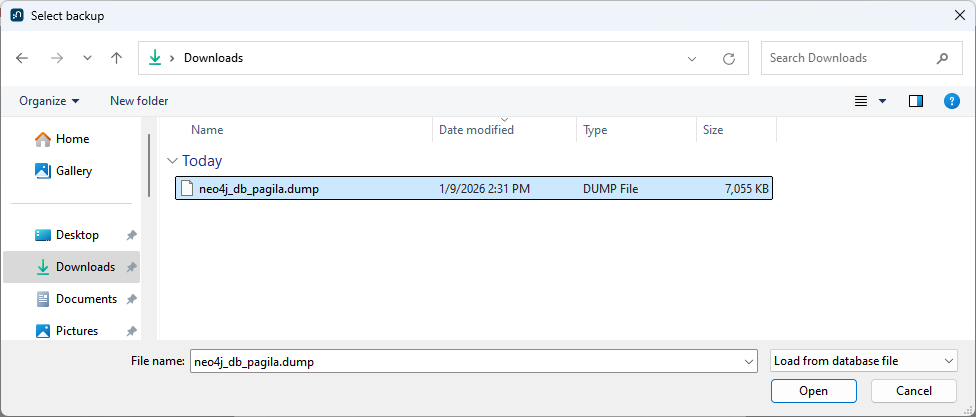
\includegraphics[width=.85\textwidth]{screen38.png}
\end{center}

\item Then, click the ''Create'' button to create the database.

\begin{center}
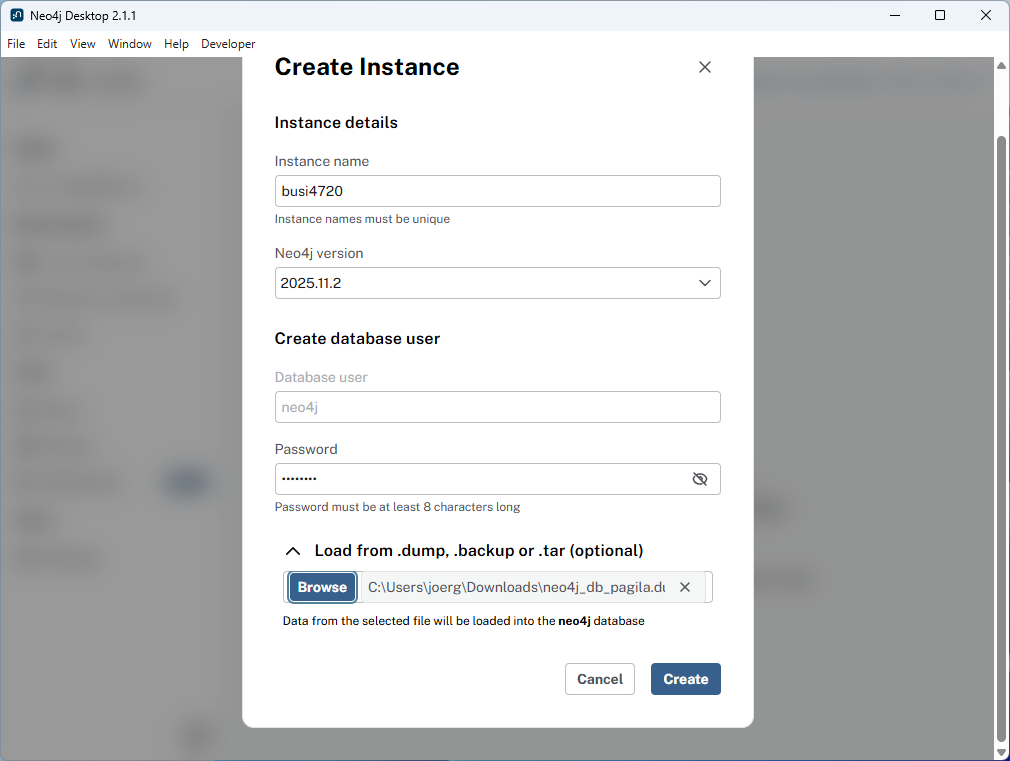
\includegraphics[width=.85\textwidth]{screen39.png}
\end{center}

\item Neo4J will create a new database and install the Pagila data into it. This may take a few minutes.


\begin{center}
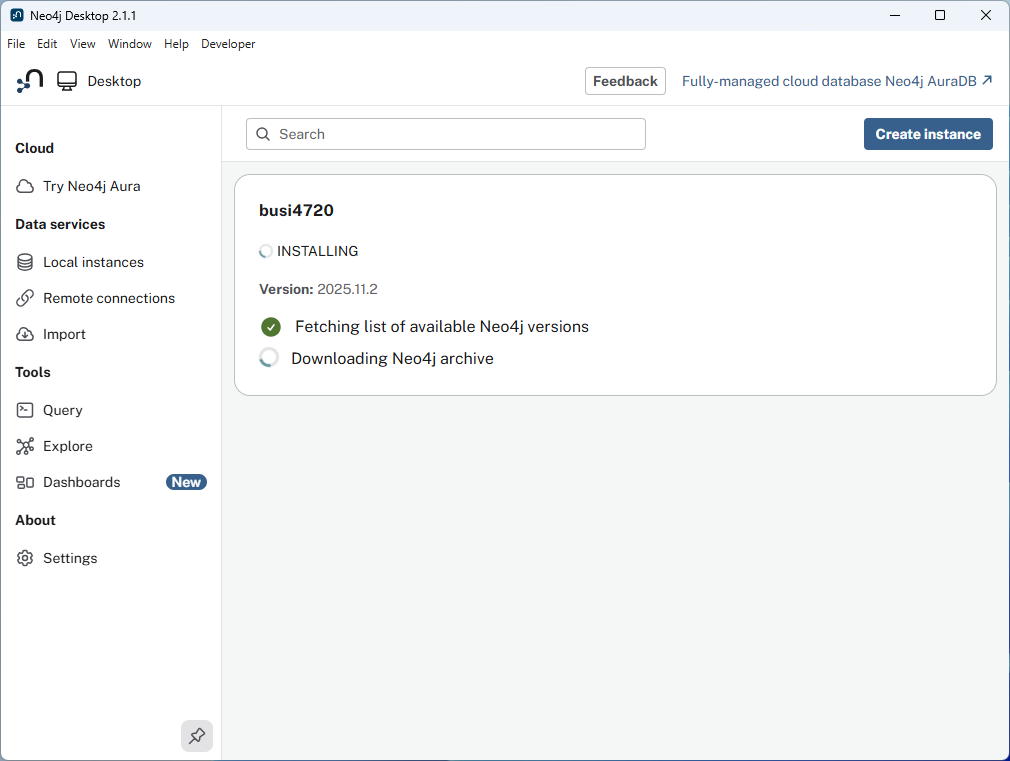
\includegraphics[width=.85\textwidth]{screen40.png}
\end{center}

\clearpage
\item Once the database is created, click the ''Connect'' button to connect to it in query mode.

\begin{center}
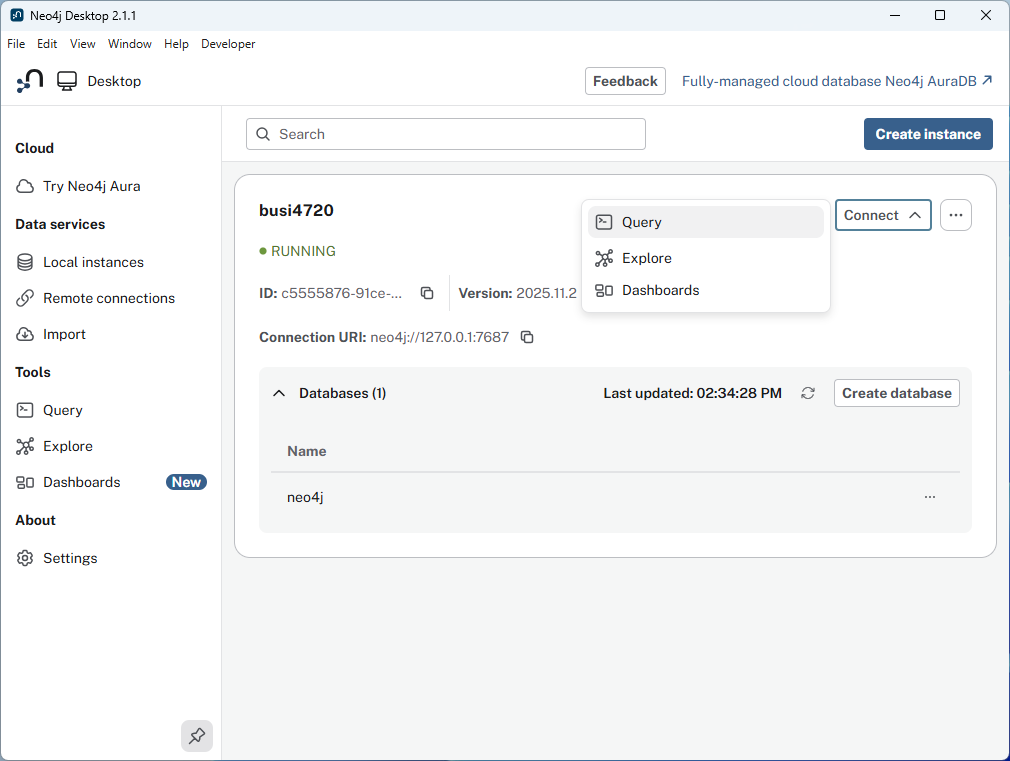
\includegraphics[width=.85\textwidth]{screen41.png}
\end{center}

\item The Neo4J desktop application will read the database contents, prepare a summary of nodes and relationships, and will present a query window.

\begin{center}
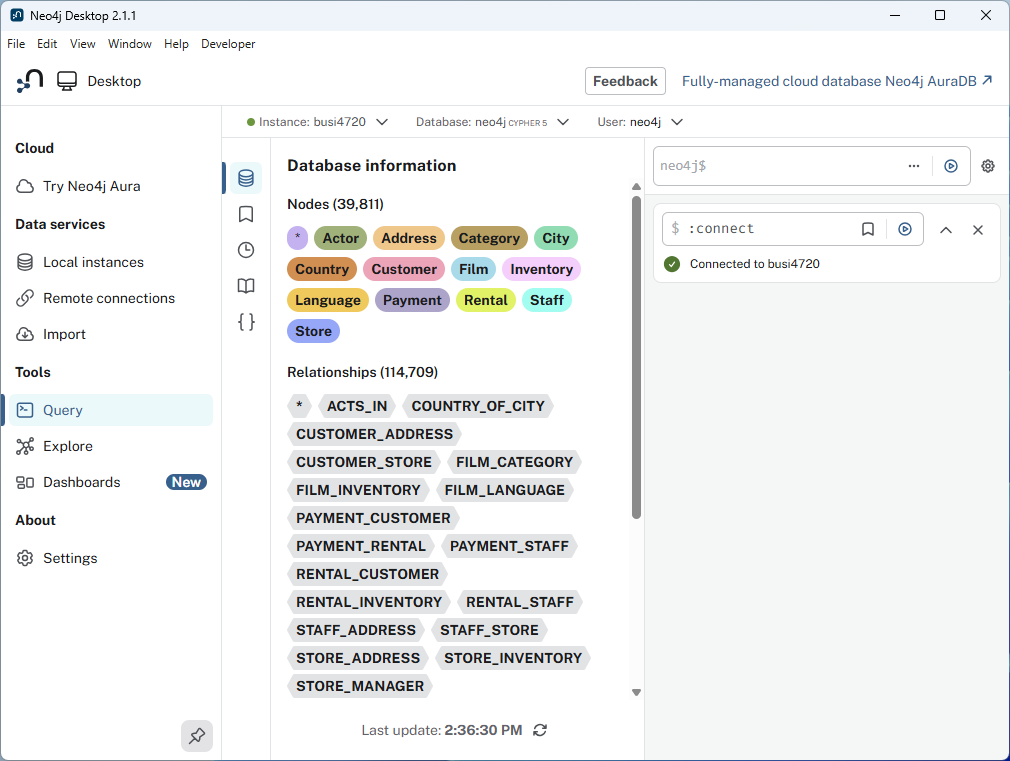
\includegraphics[width=.85\textwidth]{screen42.png}
\end{center}

\begin{infobox}
When starting the Neo4J application again, it is possible that the local database instance is not running. In this case, click the ''Start Instance'' button before connecting to the database.

\begin{center}
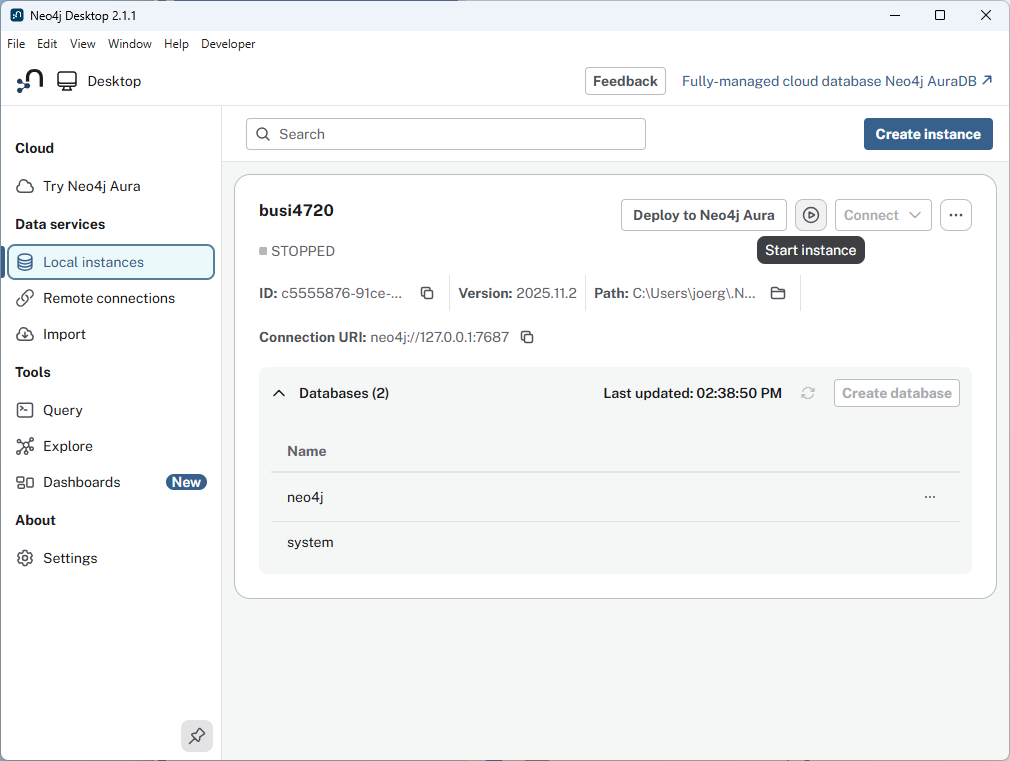
\includegraphics[width=\textwidth]{screen43.png}
\end{center}
\end{infobox}

\end{itemize}

\clearpage
\section{Installing Software on MacOS}

The Python and R software systems are available on both Windows and Mac. While a number of advanced development environments and graphical notepad user interfaces exist, it is best to initially use the basic installation. 

\subsection{Installing R}

The R software can be downloaded from the Comprehensive R Archive Network (''CRAN''). CRAN is a repository of the R software itself as well as most of the libraries or packages.

\begin{resourcebox}
You can find the Comprehensive R Archive Network (''CRAN'') here:\\

\vspace{.5\baselineskip}
\url{htts://cran.r-project.org}
\end{resourcebox}

\begin{itemize}
\item On the CRAN website, navigate to the download page for Windows. Select the latest ''base'' version of R to download. At the time of writing, this was version 4.5.2.

\begin{center}
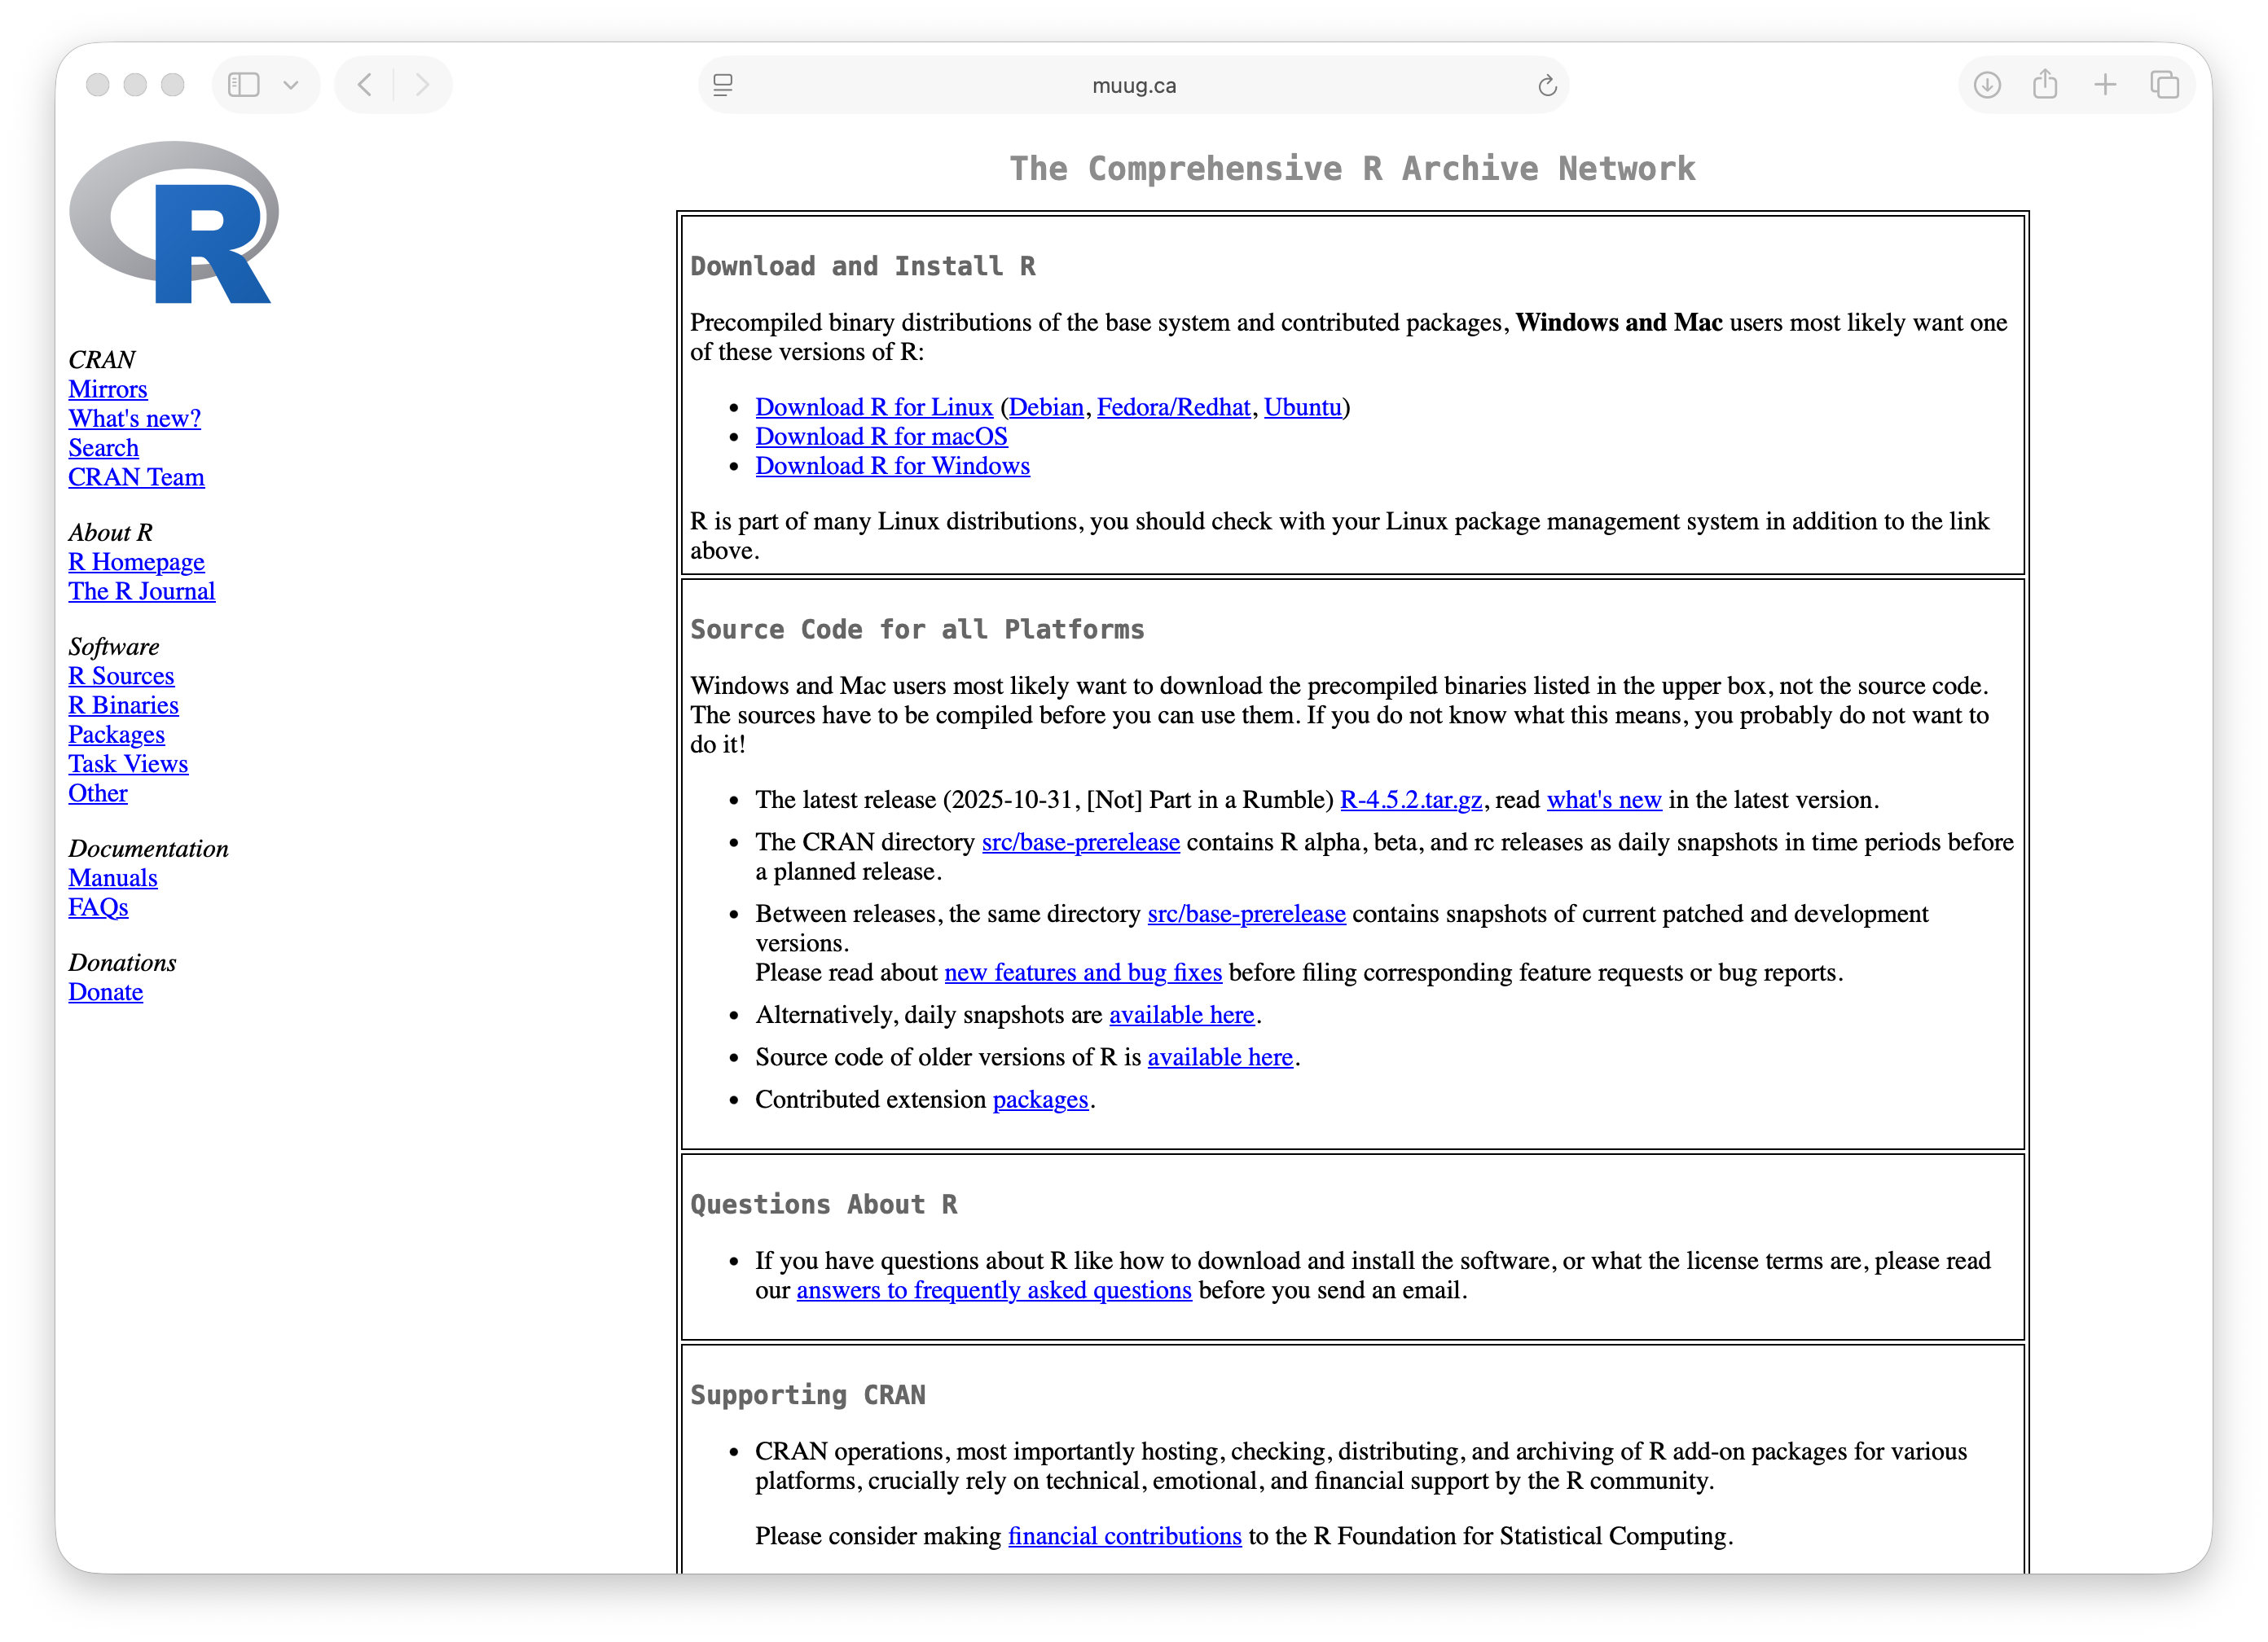
\includegraphics[width=.95\textwidth]{screen44.png}
\end{center}

\clearpage
\item Select the download file that applies to your Apple computer. Newer Apple computers (since approx. 2021) will use Apple silicom (M1, M2, etc.). 

\begin{center}
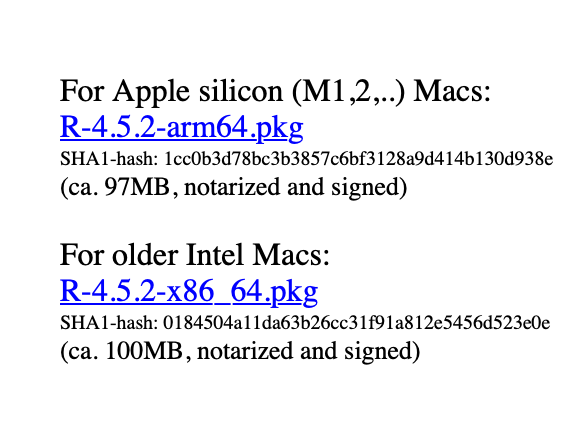
\includegraphics[width=.55\textwidth]{screen45.png}
\end{center}

\item When your download has finished, click on the downloaded file to open it and begin the installation.

\begin{center}
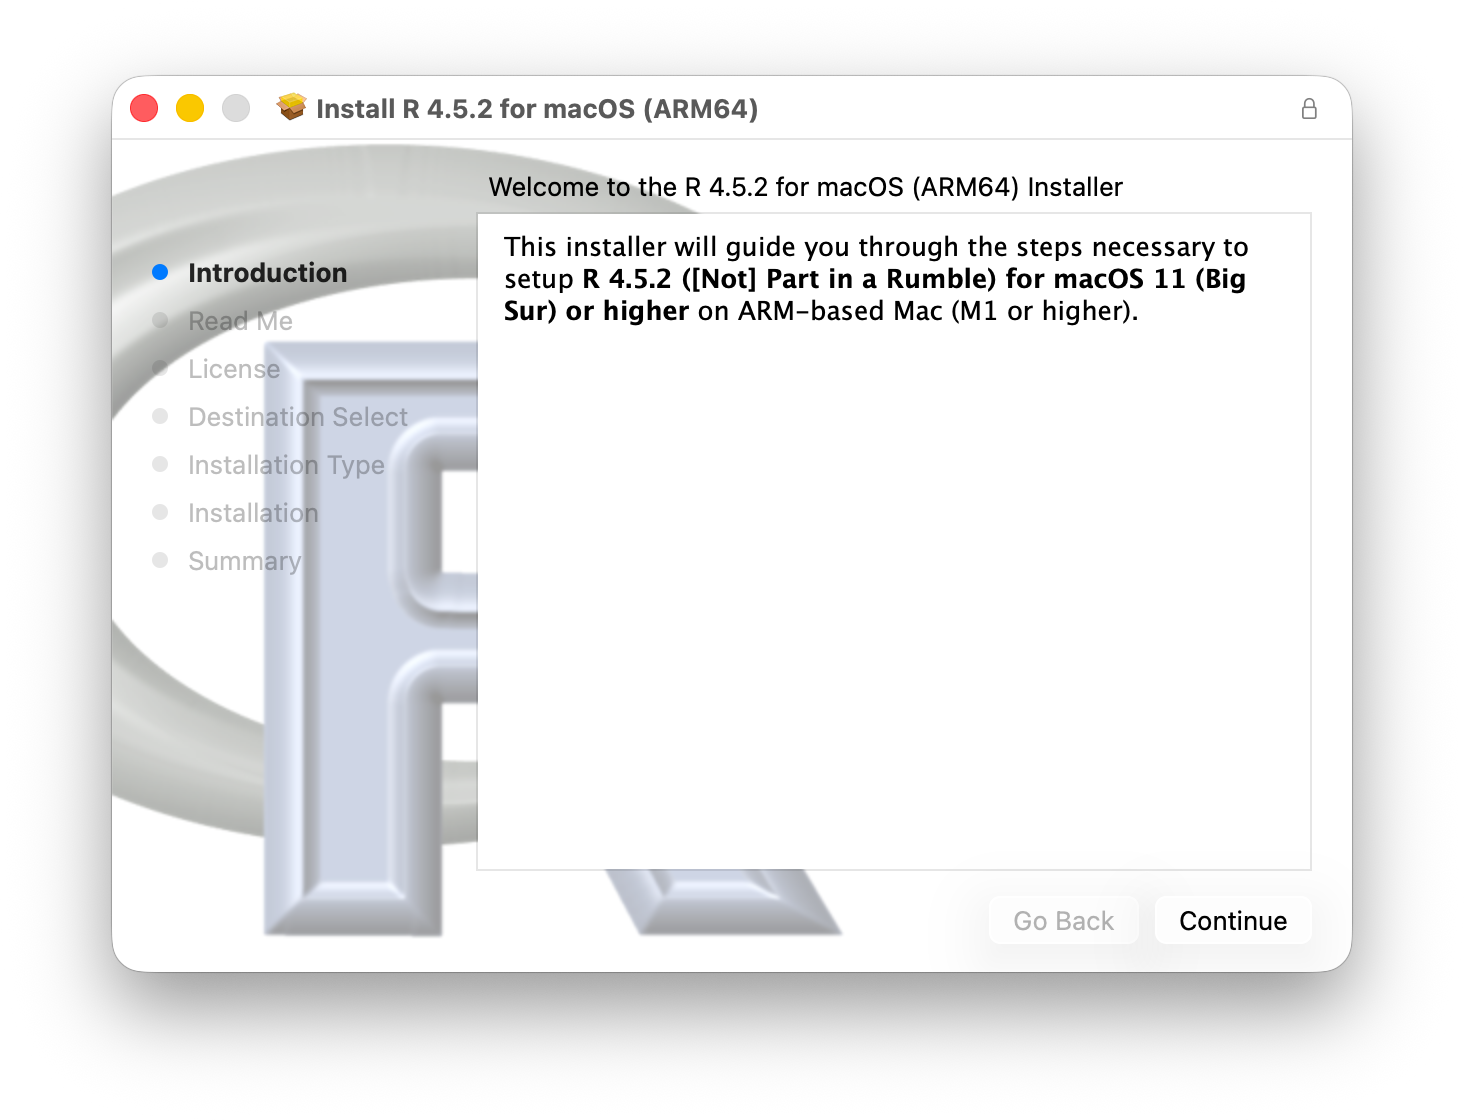
\includegraphics[width=.95\textwidth]{screen46.png}
\end{center}

Click the ''Continue button'' for each step of the installation. You may be prompted to enter your computer's password to allow the installation. 

\clearpage
\item Once the installer finishes, click the ''Close'' button.

\begin{center}
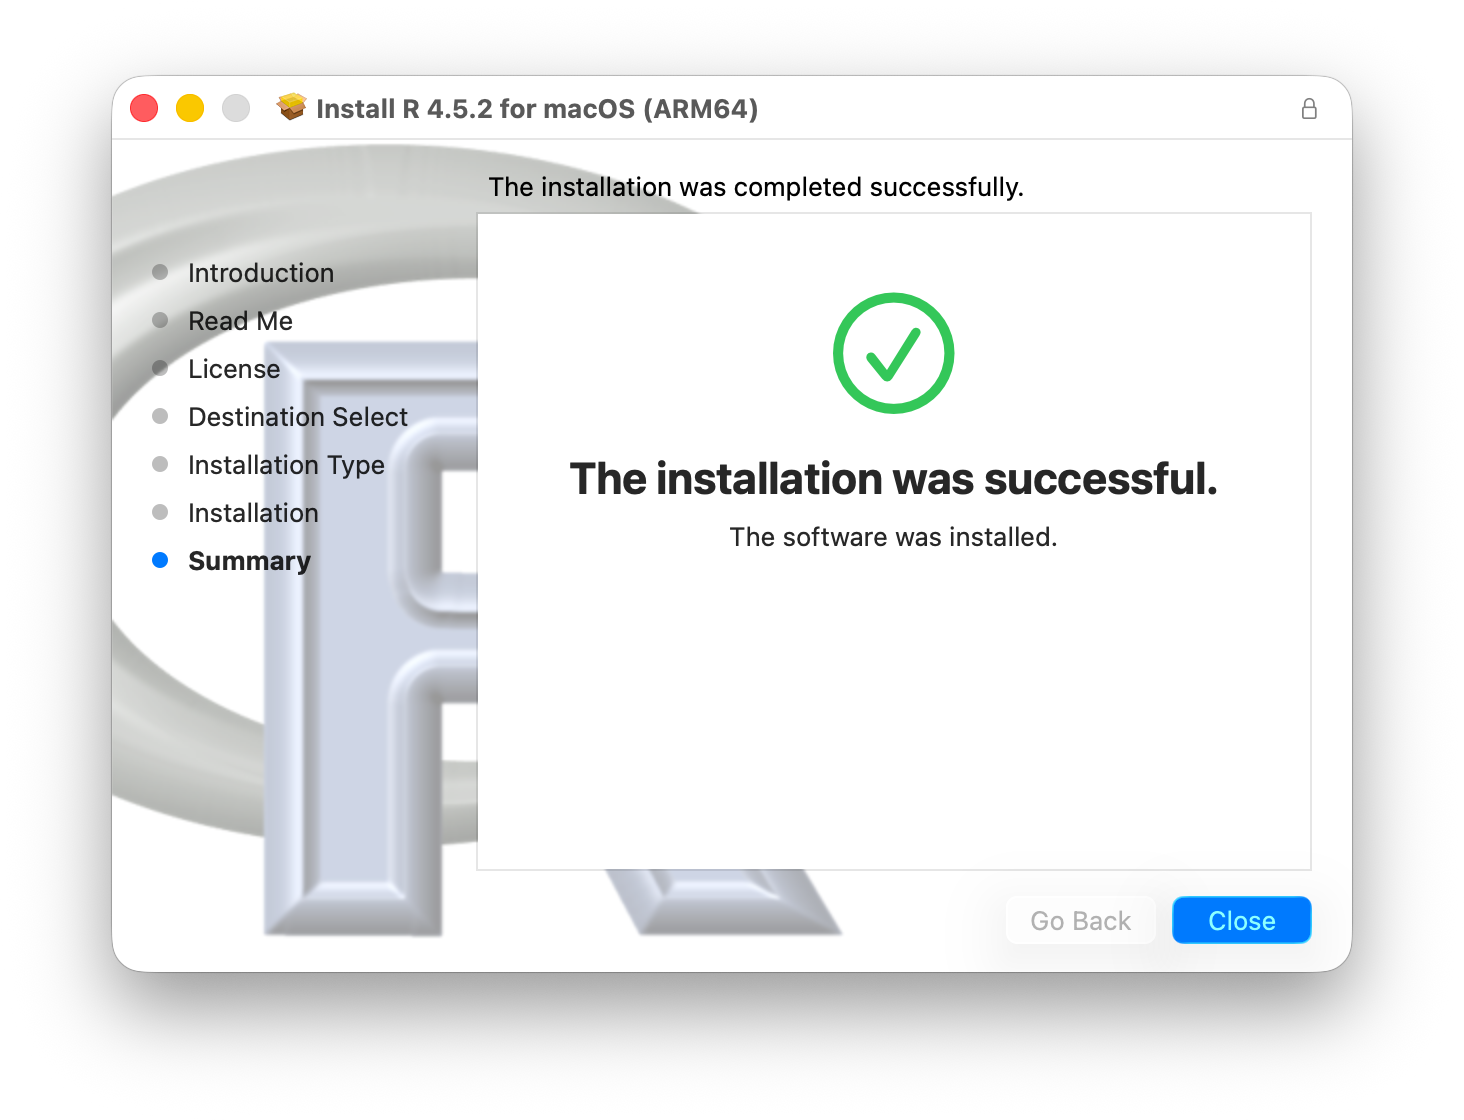
\includegraphics[width=.95\textwidth]{screen47.png}
\end{center}

\item Using the Finder, navigate to the Applications folder, find the R software and start it.

\begin{center}
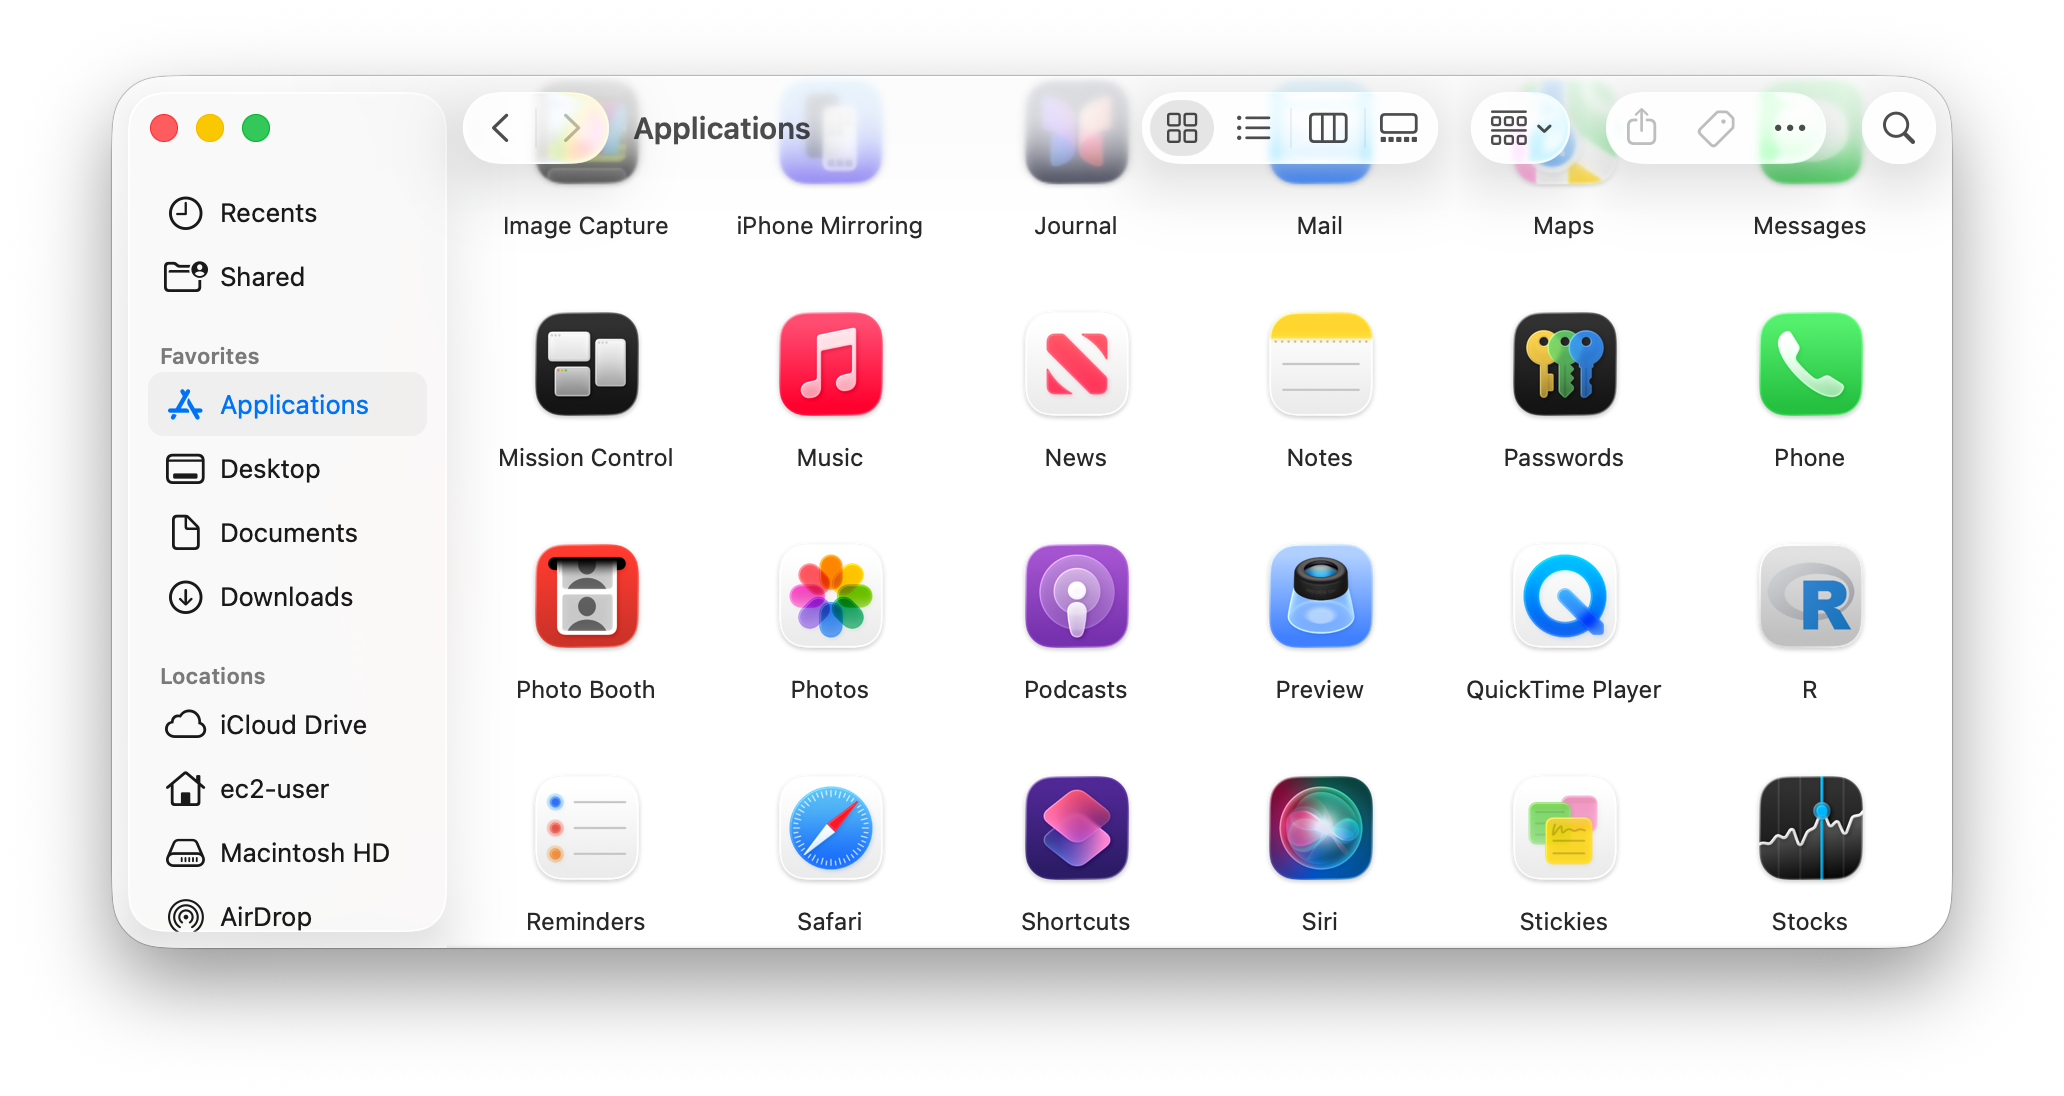
\includegraphics[width=.95\textwidth]{screen48.png}
\end{center}

\clearpage
\item You will see the R graphical user interface. You can enlarge the inner window titled ''R Console'' using the button in the top right corner of its window frame.

\begin{center}
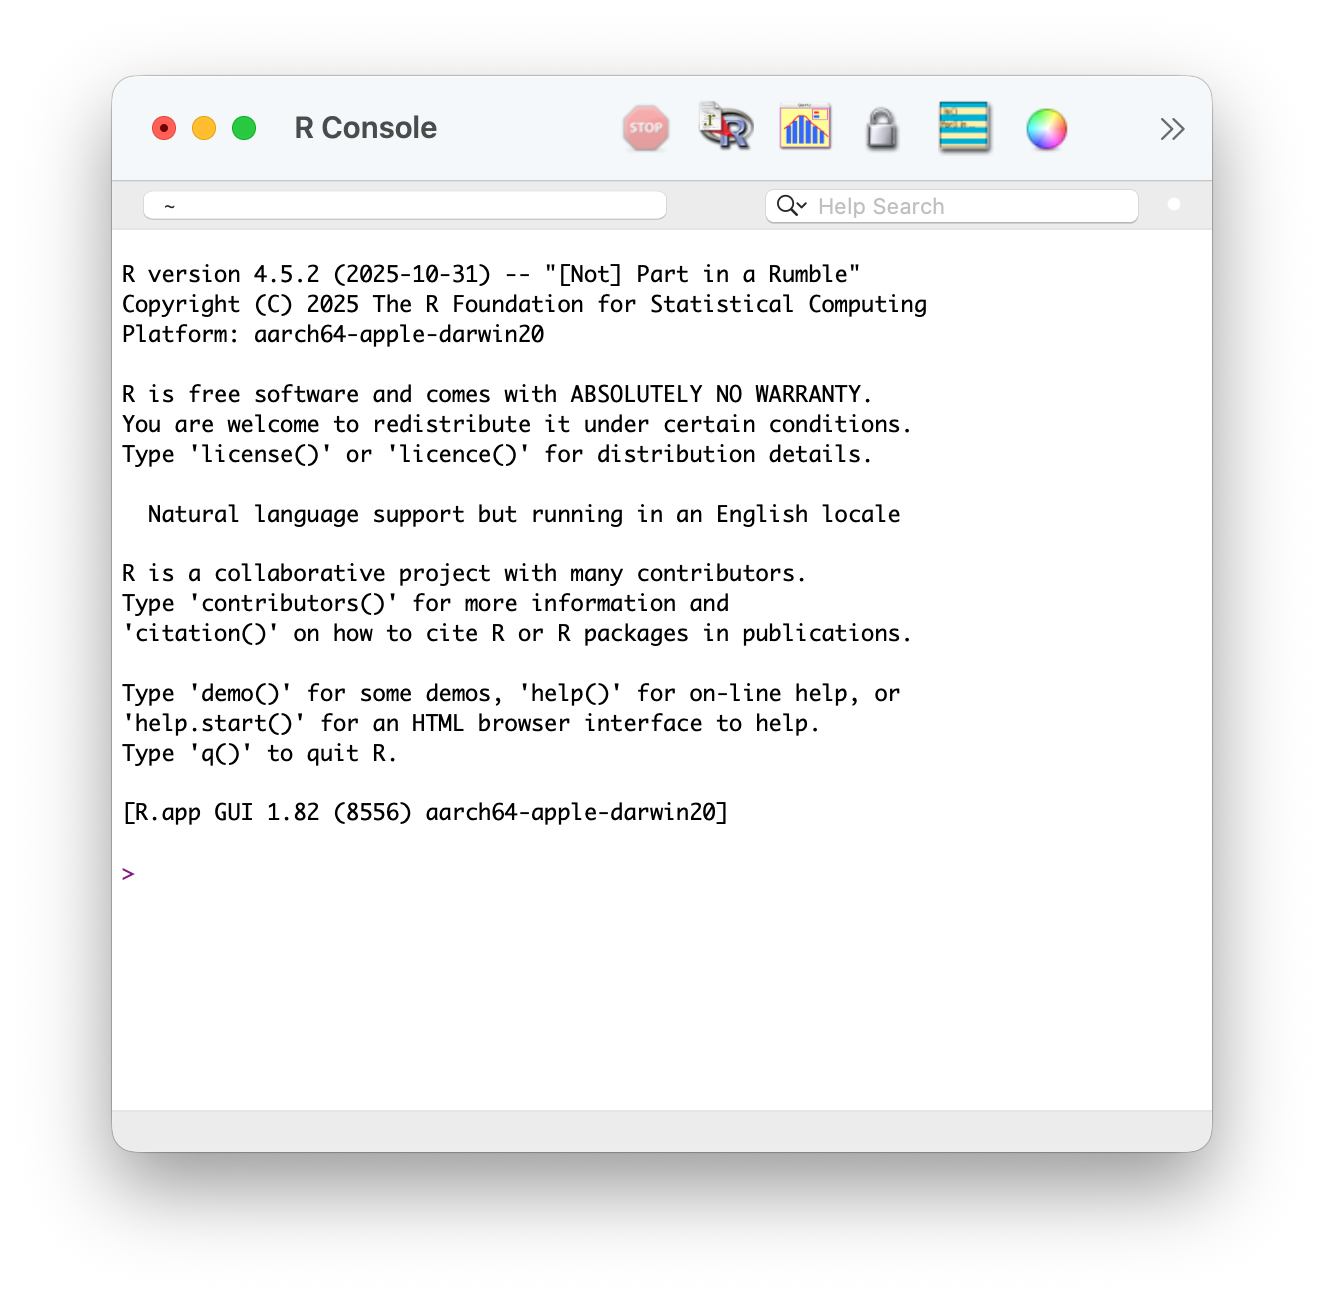
\includegraphics[width=.85\textwidth]{screen49.png}
\end{center}

\item Copy and paste the following R command into the R window. Then, hit the enter key on your keyboard to execute it. This command will install the R packages used in this book.

\begin{Rcode}
install.packages(c('tidyverse', 'boot', 'zoo', 'astsa', 
'devtools', 'fGarch', 'ggpattern', 'scales', 'ISLR2', 
'class', 'glmnet', 'e1071', 'ROCR', 'sqldf', 'ggsci'))
\end{Rcode}

\begin{center}
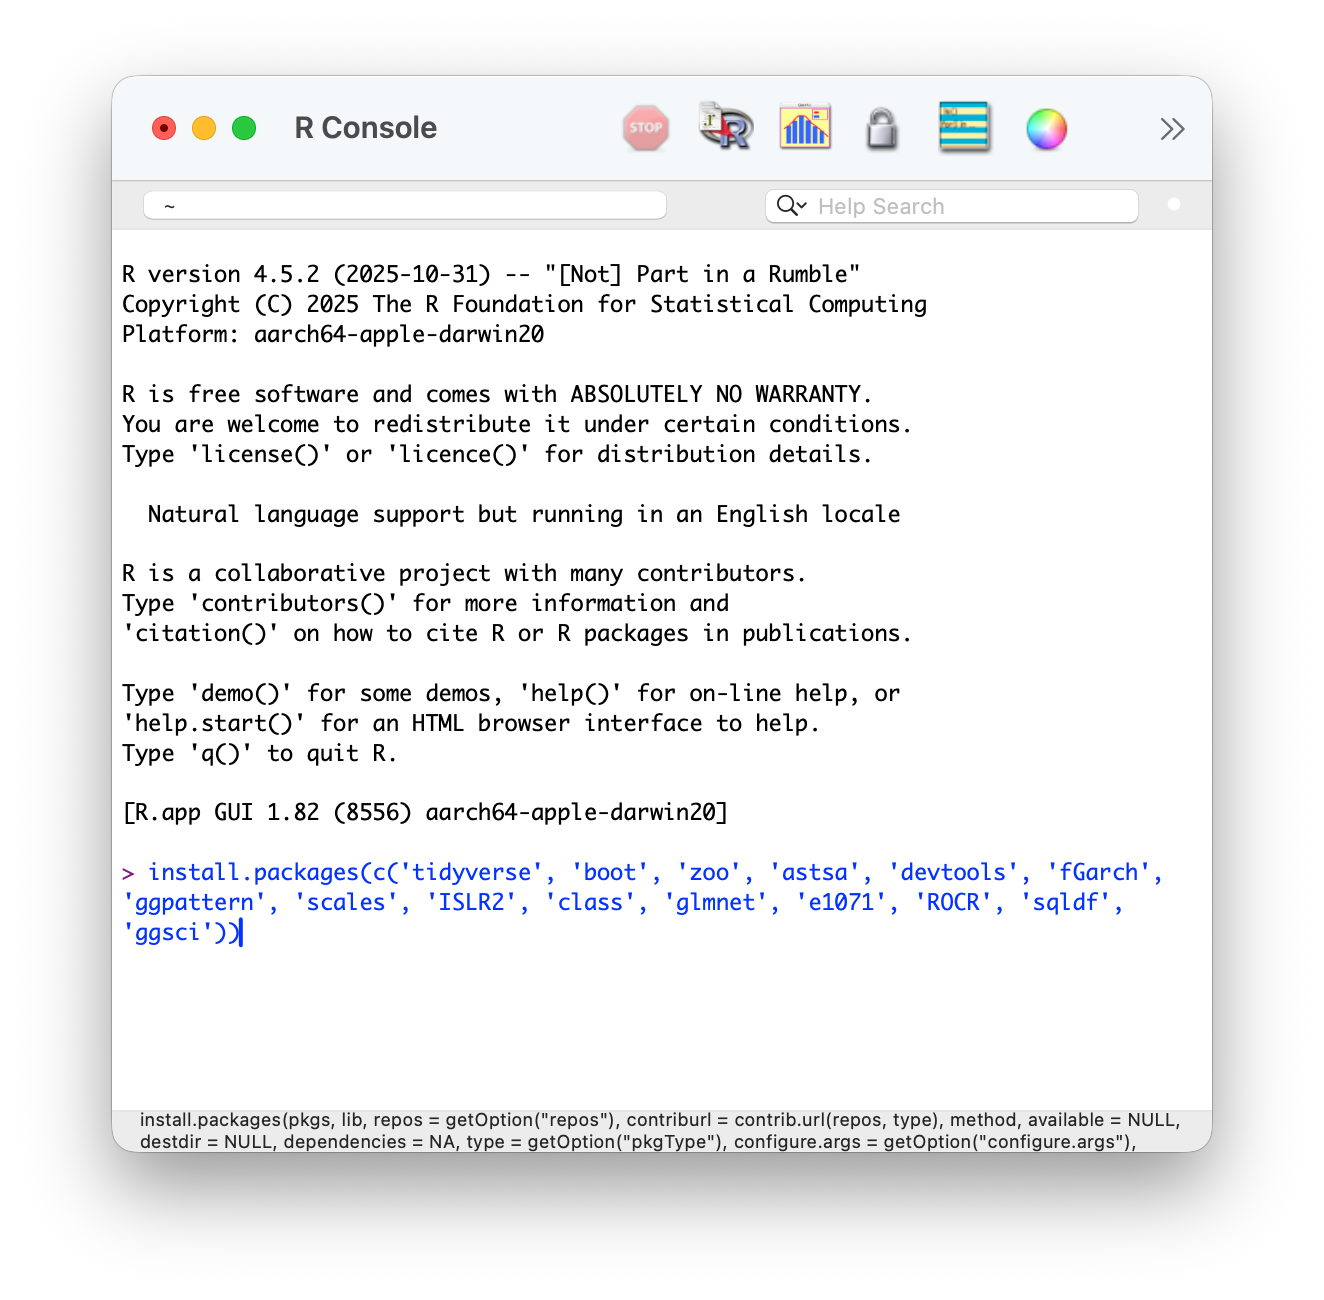
\includegraphics[width=.85\textwidth]{screen50.png}
\end{center}

You will be asked to choose a CRAN mirror. The software on all mirrors is identical but choosing one that is geographically close greatly improves the download speed.

\begin{center}
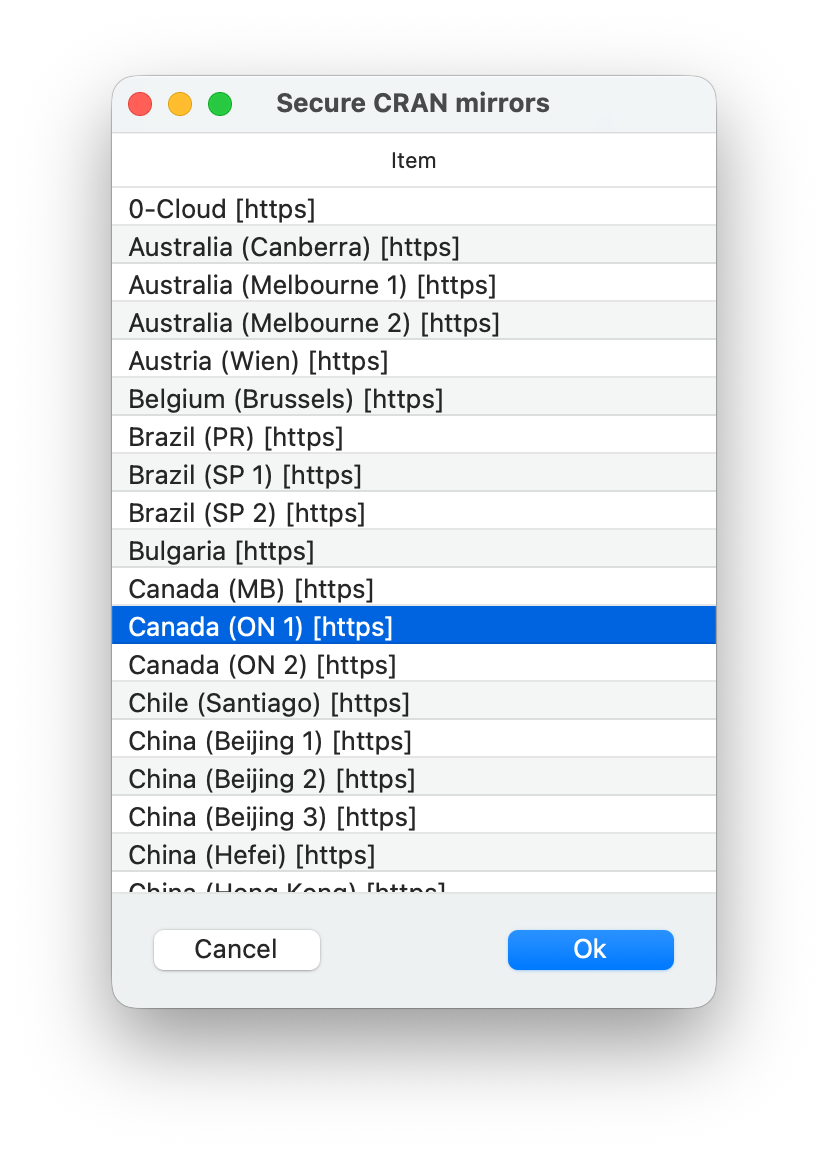
\includegraphics[width=.45\textwidth]{screen51.png}
\end{center}

\item You can quit R by executing the following command in the R window or simply by closing the R window itself.

\begin{Rcode}
quit()
\end{Rcode}

\end{itemize}

\begin{infobox}
The downloaded versions of the R libraries may be newer than those used for the writing of this book. While it is not expected that their behaviour will change, you may wish to consult the libraries' manuals if it does.
\end{infobox}


\clearpage
\subsection{Installing Python}

\begin{resourcebox}
Python is available for all major computer systems from its web site. \\

\url{https://www.python.org}
\end{resourcebox}

To install Python follow these instructions.

\begin{itemize}

\item With your web browser, navigate to the Python home page.

\begin{center}
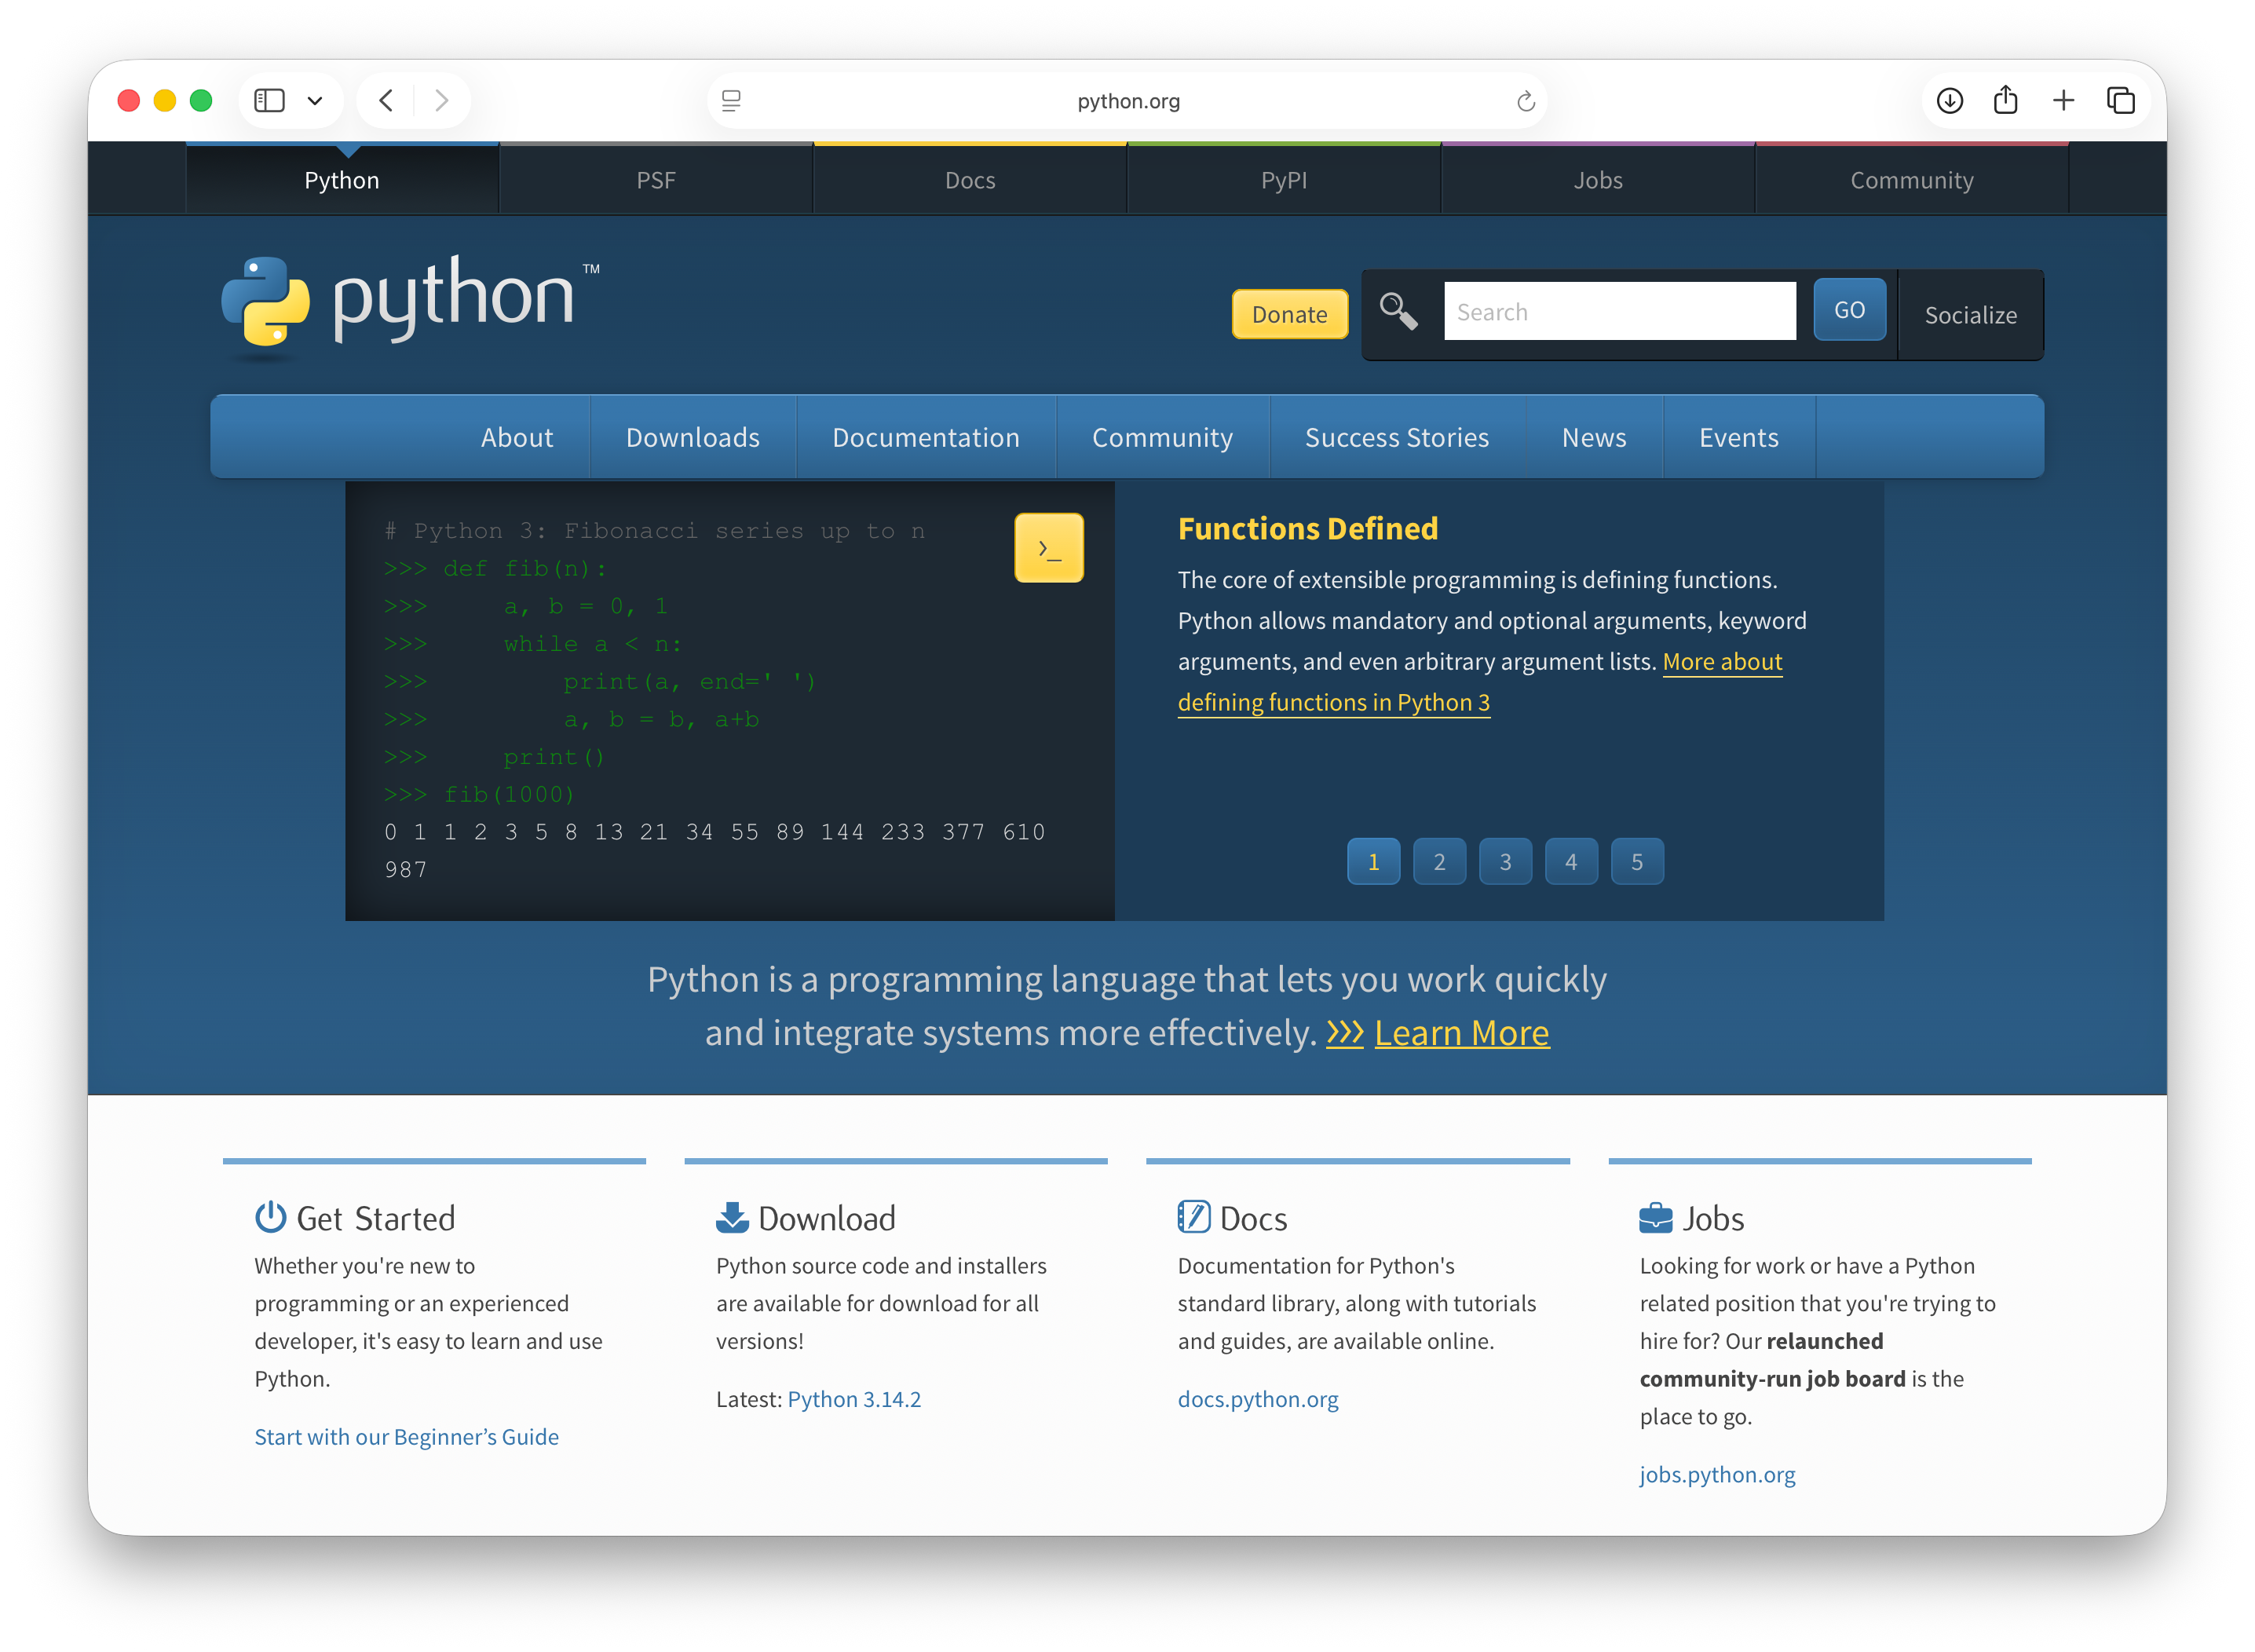
\includegraphics[width=.95\textwidth]{screen52.png}
\end{center}

\item Navigate to the download page for Apple MacOS systems. 

\begin{center}
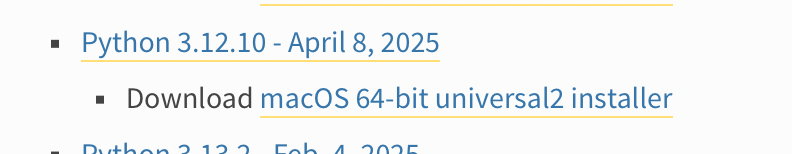
\includegraphics[width=.75\textwidth]{screen53.png}
\end{center}

\begin{infobox}
Some Python packages may not be configured to work with the latest version of Python. It is recommended that you install a slightly older version. For example, at the time of writing, version 3.14 was the latest, but version 3.12 was still being maintained and chosen for this tutorial. 
\end{infobox}

\item Once the download has completed, click on the downloaded file to begin the installation of Python.

\begin{center}
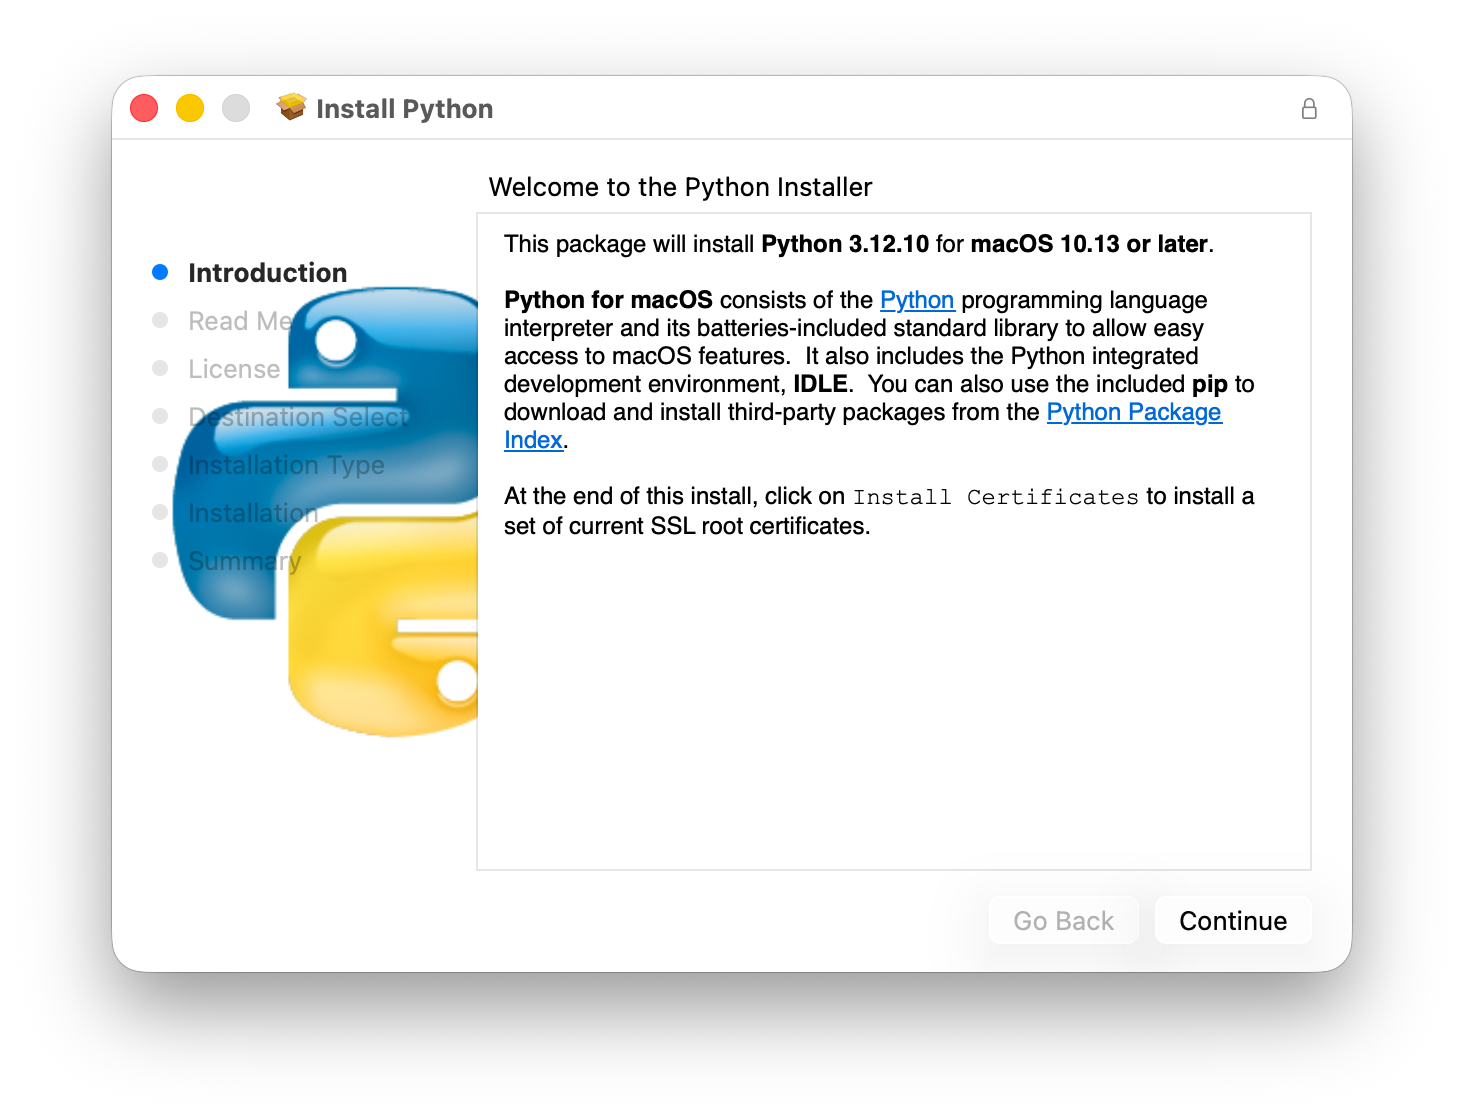
\includegraphics[width=.95\textwidth]{screen54.png}
\end{center}

\clearpage
\item Click the ''Continue'' button on each form of the installer window and then click ''Install'' to begin the installation. You do not need to customize or change any of the default options.

\begin{center}
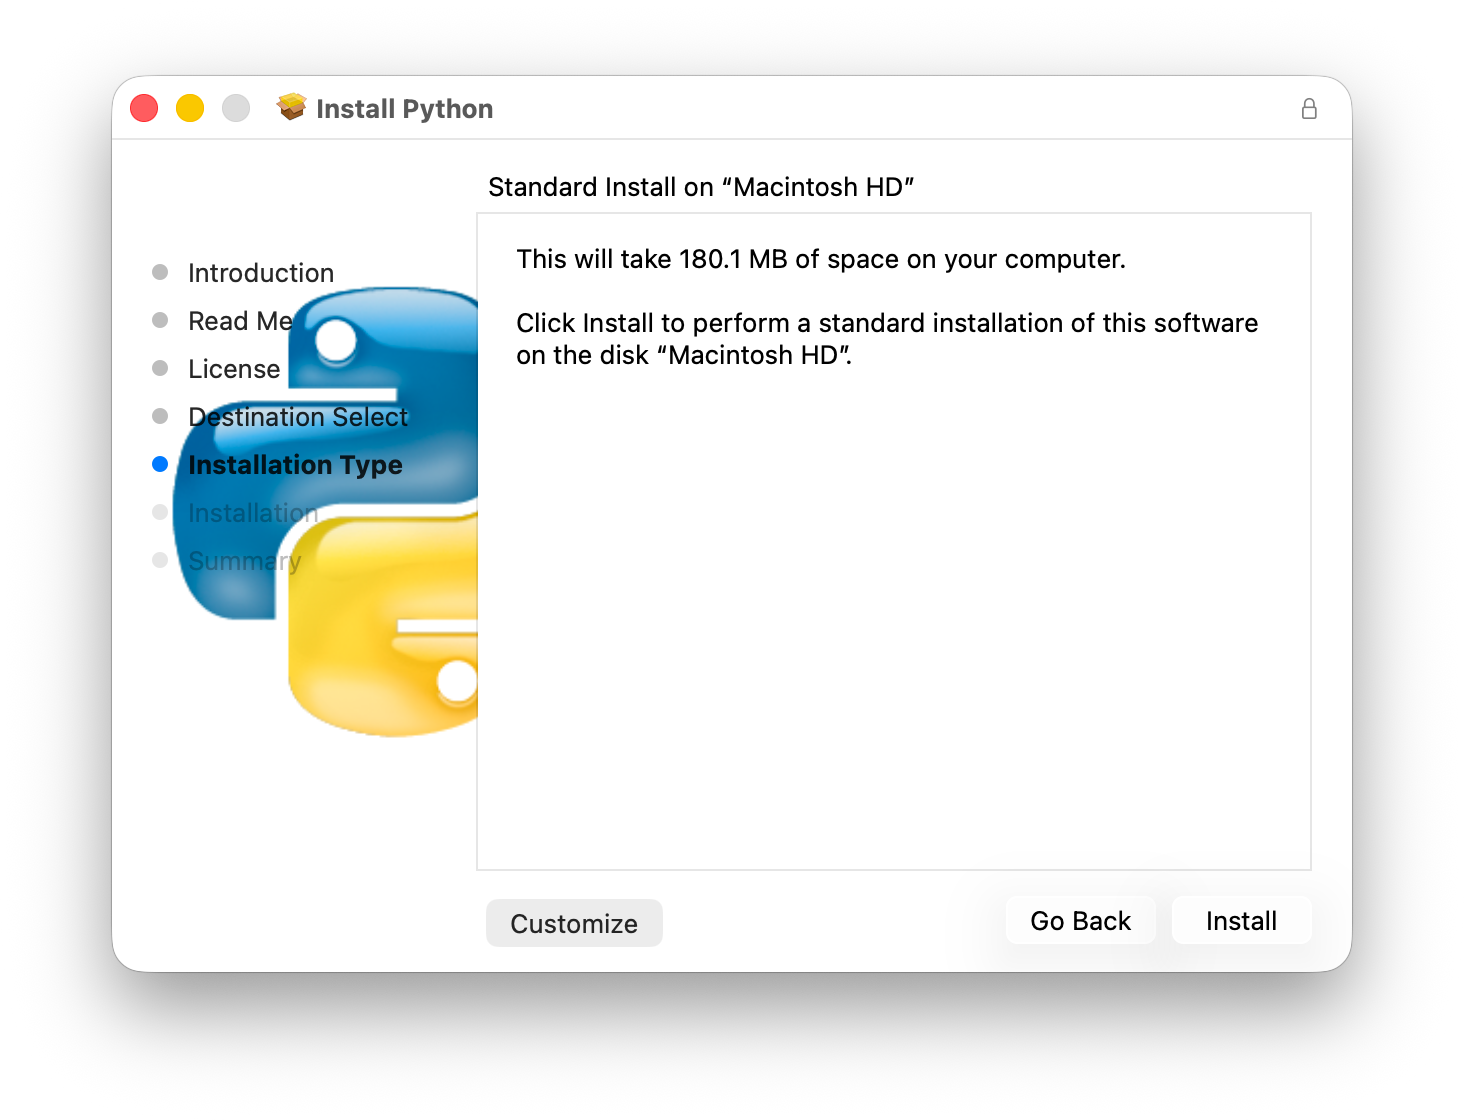
\includegraphics[width=.95\textwidth]{screen55.png}
\end{center}

You may be asked to provide your computer's password to allow the installation to proceed.

\begin{center}
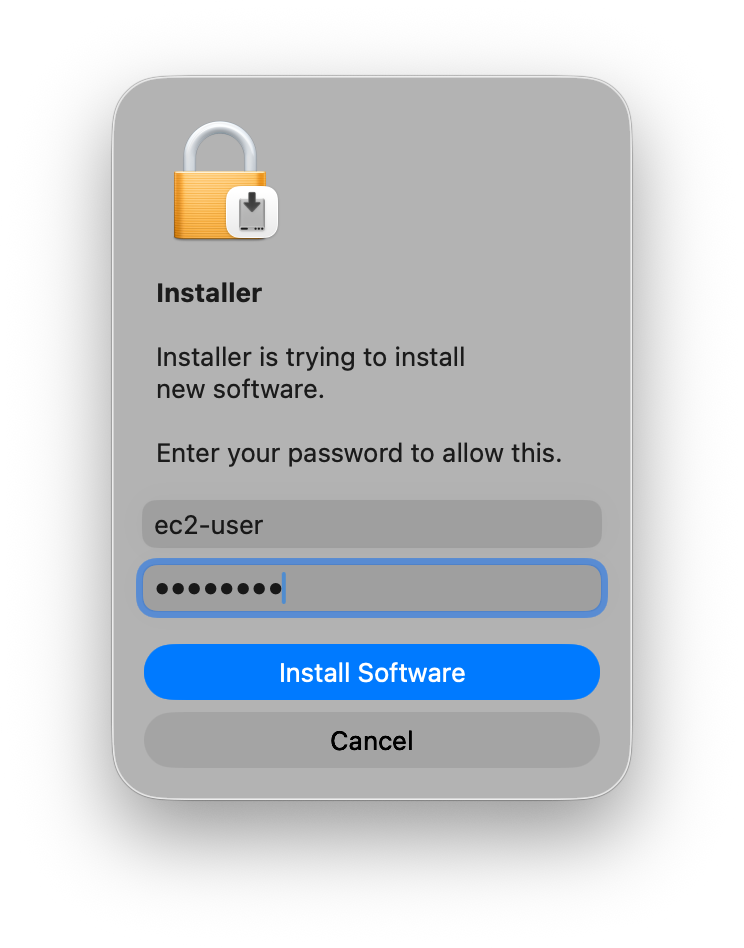
\includegraphics[width=.45\textwidth]{screen56.png}
\end{center}

\item Once the installation is complete, click the ''Close'' button to exit the installer.

\item Using your Finder, navigate to your Applications, then into the Utilities folder. Doubleclick the Terminal application to open it.

\begin{center}
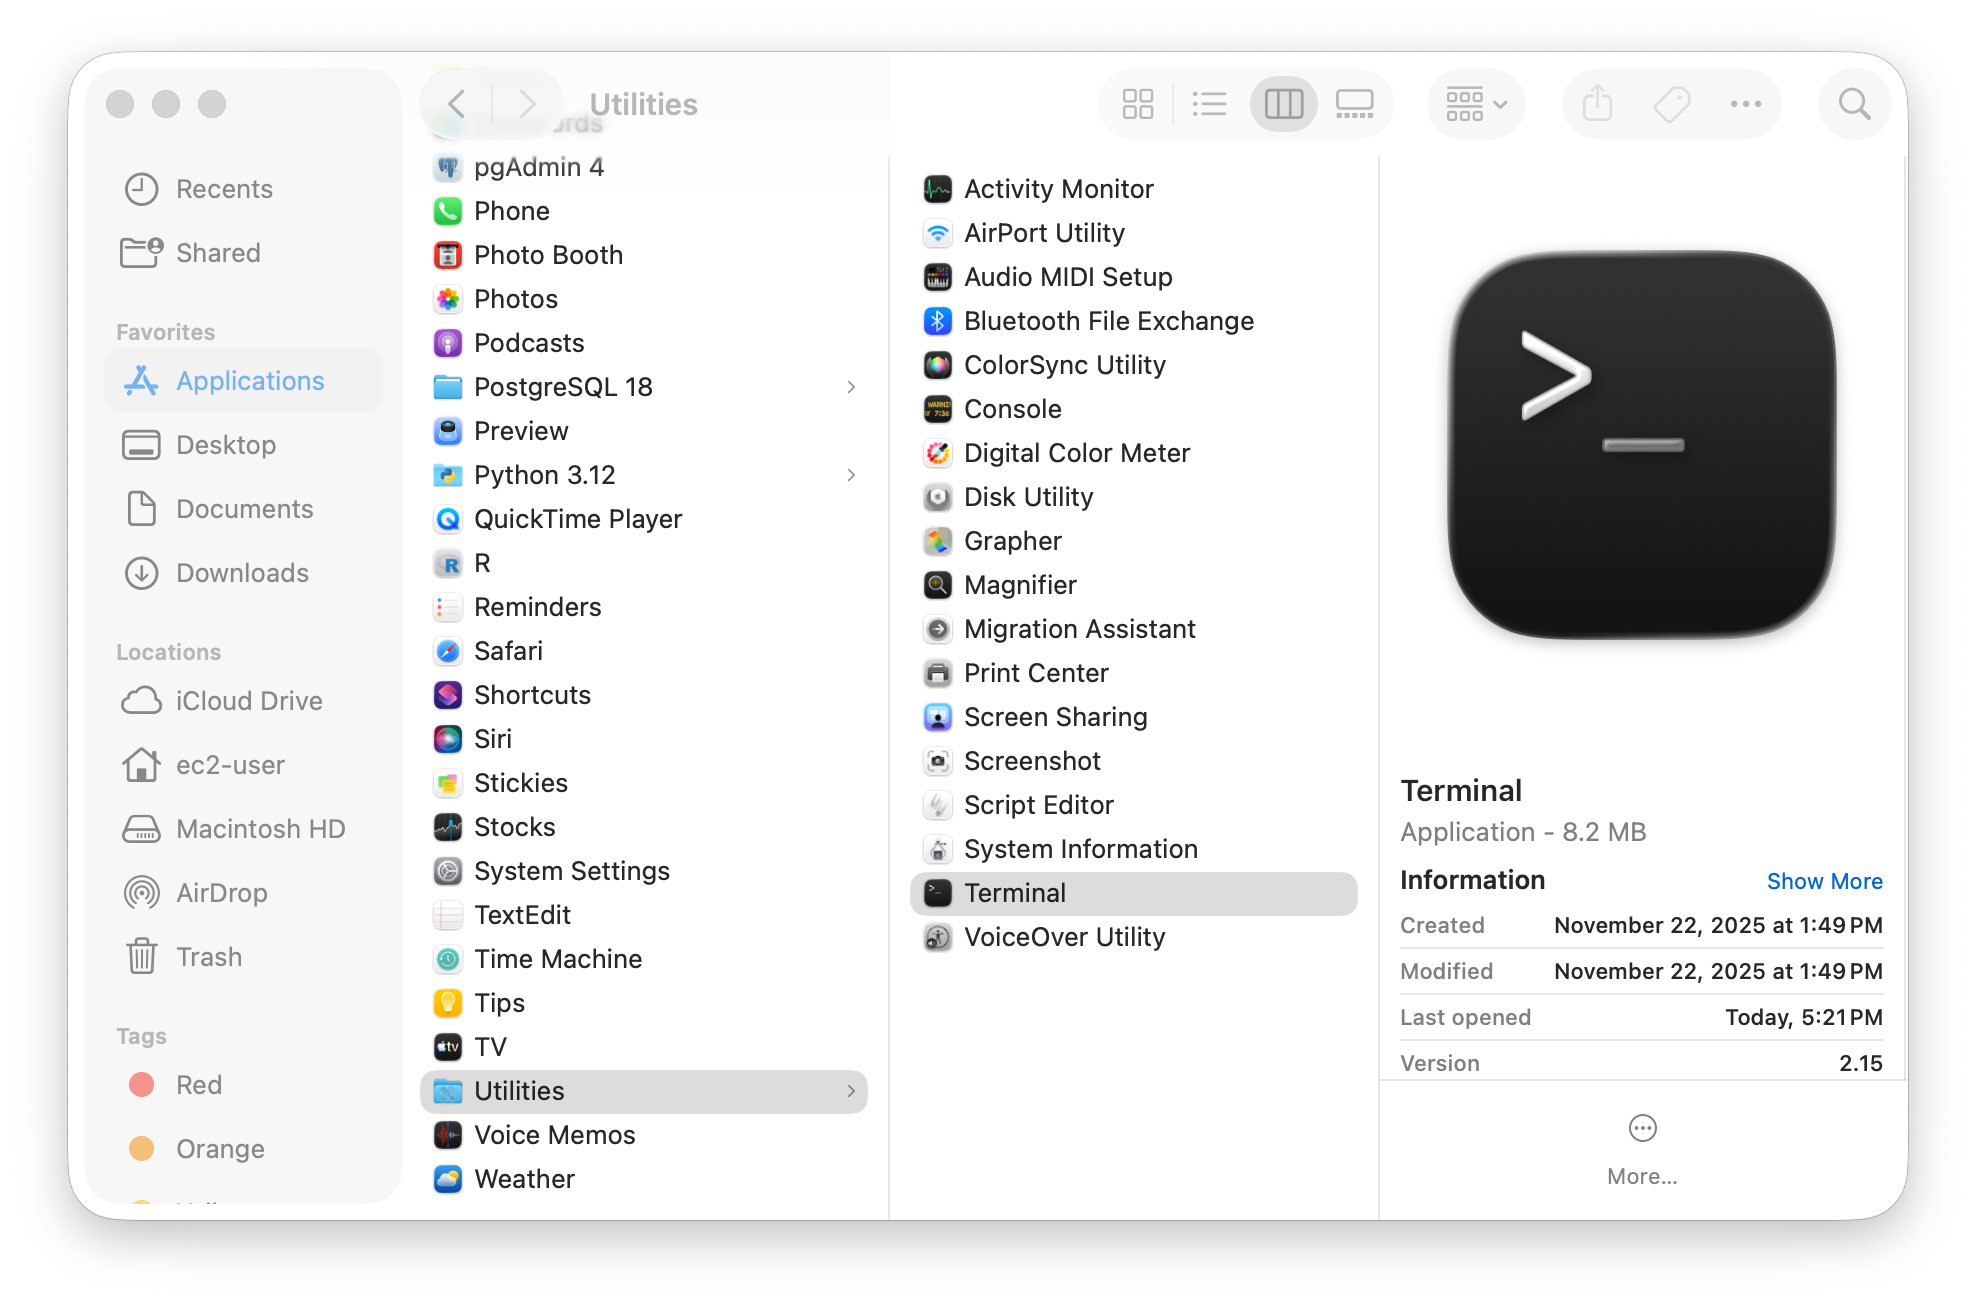
\includegraphics[width=.95\textwidth]{screen57.png}
\end{center}

\item Copy and paste the following commands into this window and hit the enter key on your keyboard to execute them. This will set up a Python virtual environment to install the required Python packages into.

\begin{bashcode}
python3 -m venv venv
source venv/bin/activate
\end{bashcode}

\item Copy and paste the following command into this window and hit the enter key on your keyboard to execute it. This will install all Python packages used in this book and the packages they in turn depend on.

\begin{bashcode}
pip3 install -r https://www.evermann.ca/busi4720/requirements.txt
\end{bashcode}

\begin{center}
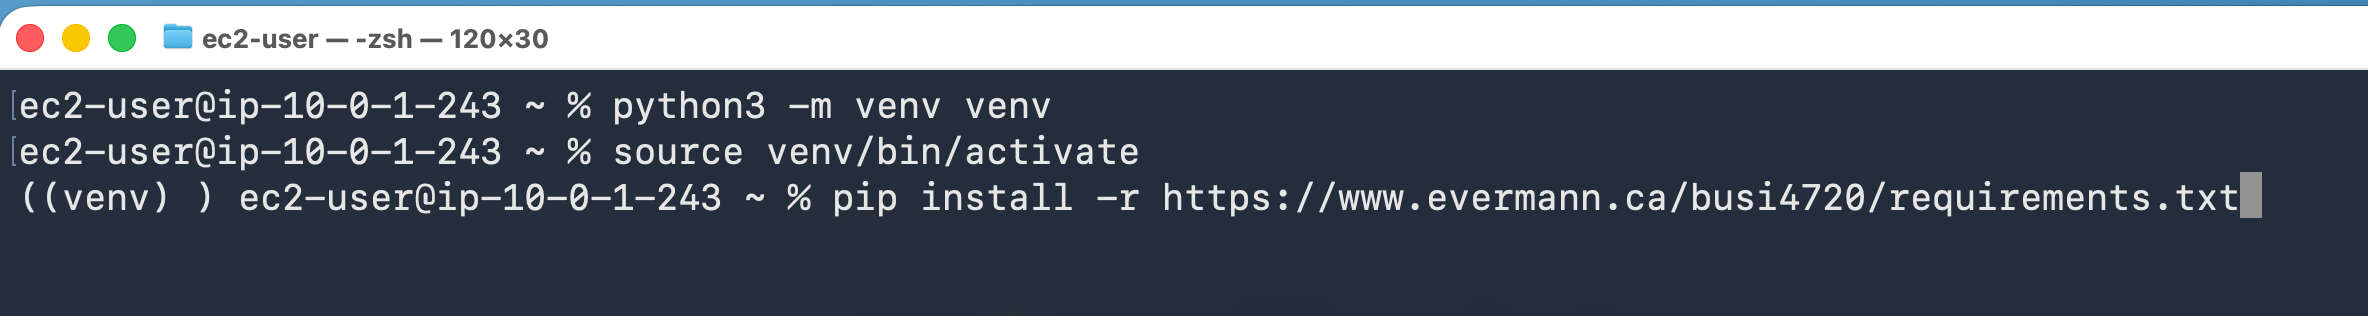
\includegraphics[width=.95\textwidth]{screen58.png}
\end{center}

\clearpage
Downloading and installing all packages will take a few minutes. You should see a success message similar to the following screenshot.

\begin{center}
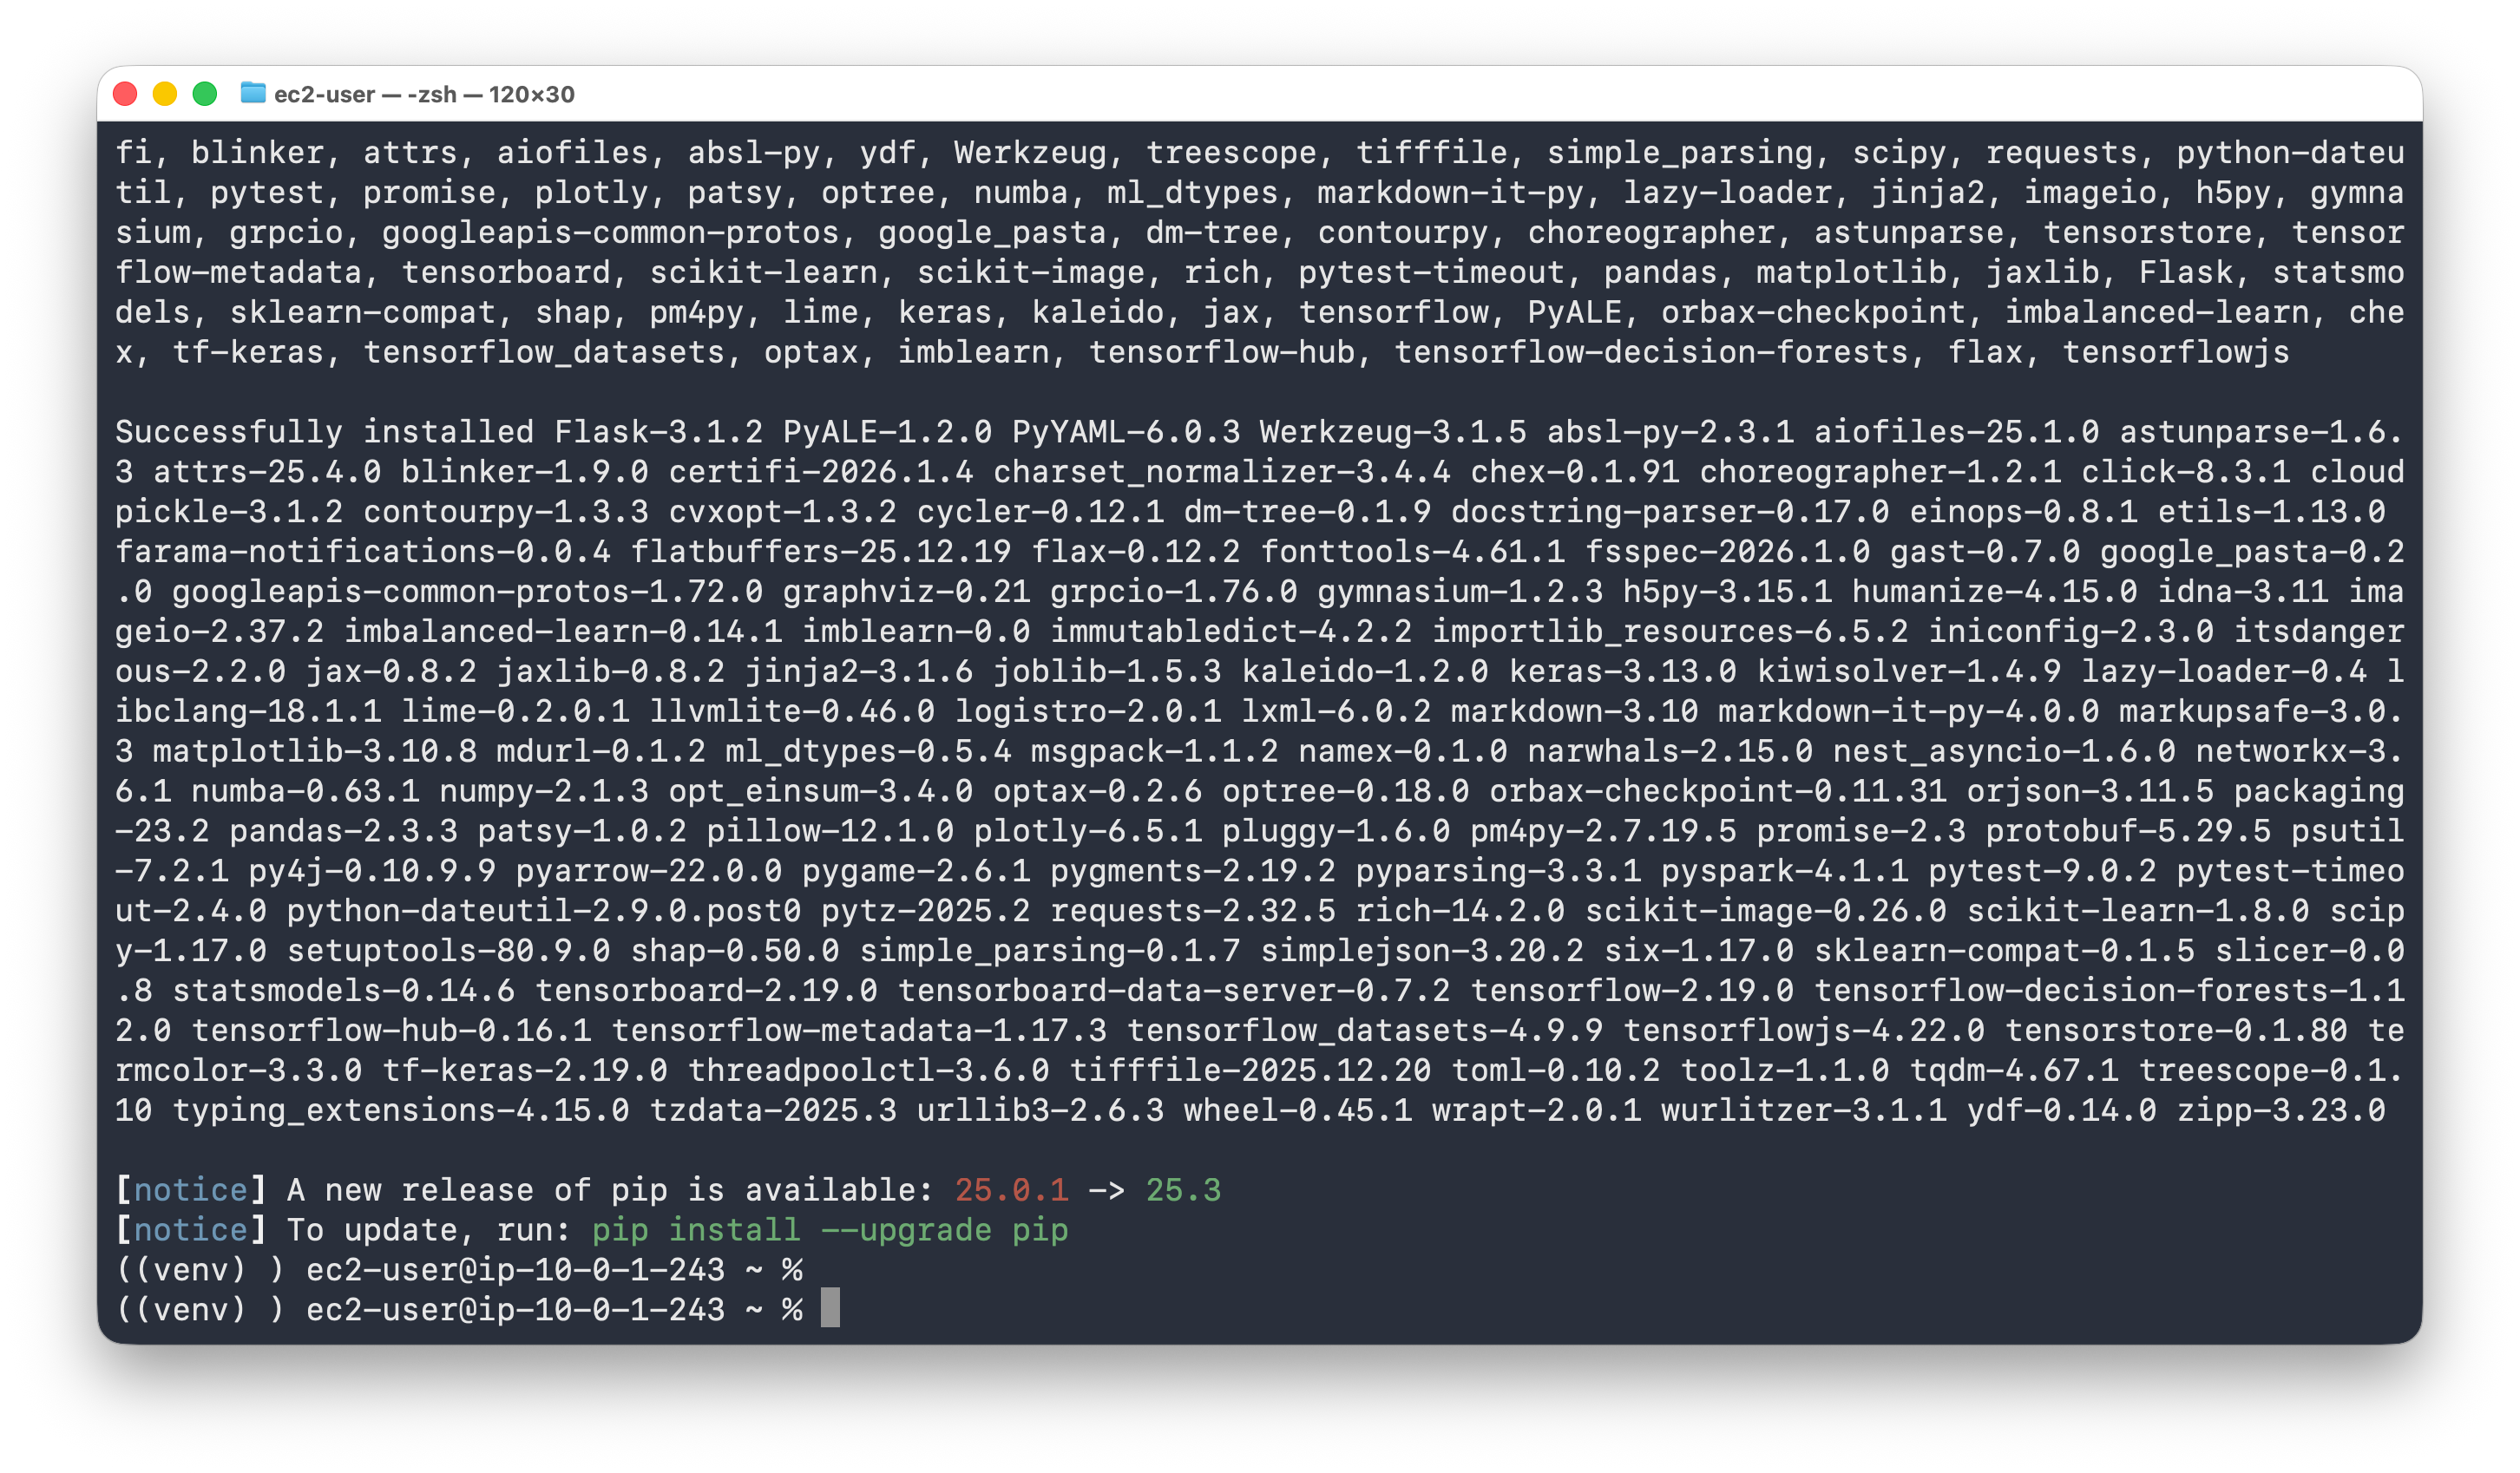
\includegraphics[width=.95\textwidth]{screen59.png}
\end{center}

\item Deactivate the Python virtual environment using the following command:

\begin{bashcode}
deactivate
\end{bashcode}

\begin{alertbox}
To use Python, you will need to 
\begin{enumerate}
\item Start the Terminal application from your Applications/Utilities folder
\item Activate the Python virtual environment with the following command
\begin{bashcode}
source venv/bin/activate
\end{bashcode}
\item Start Python with the following command
\begin{bashcode}
python3
\end{bashcode}
\item To exit Python, enter the following Python command
\begin{pythoncode}
quit()
\end{pythoncode}
\item Close the Terminal window or application
\end{enumerate}
\end{alertbox}

\begin{infobox}
The downloaded versions of the Python packages may be newer than those used for the writing of this book. While it is not expected that their behaviour will change, you may wish to consult the packages' manuals if it does.
\end{infobox}

\end{itemize}
\clearpage
\subsection{Installing PostgreSQL}

\begin{resourcebox}
PostgreSQL is available for Windows and MacOS systems and installation applications can be found via its website. \\

\url{https://www.postgresql.org}
\end{resourcebox}

\begin{itemize}
\item Navigate to the Downloads section of the PostgreSQL website. Then select the MacOS installer.

\begin{center}
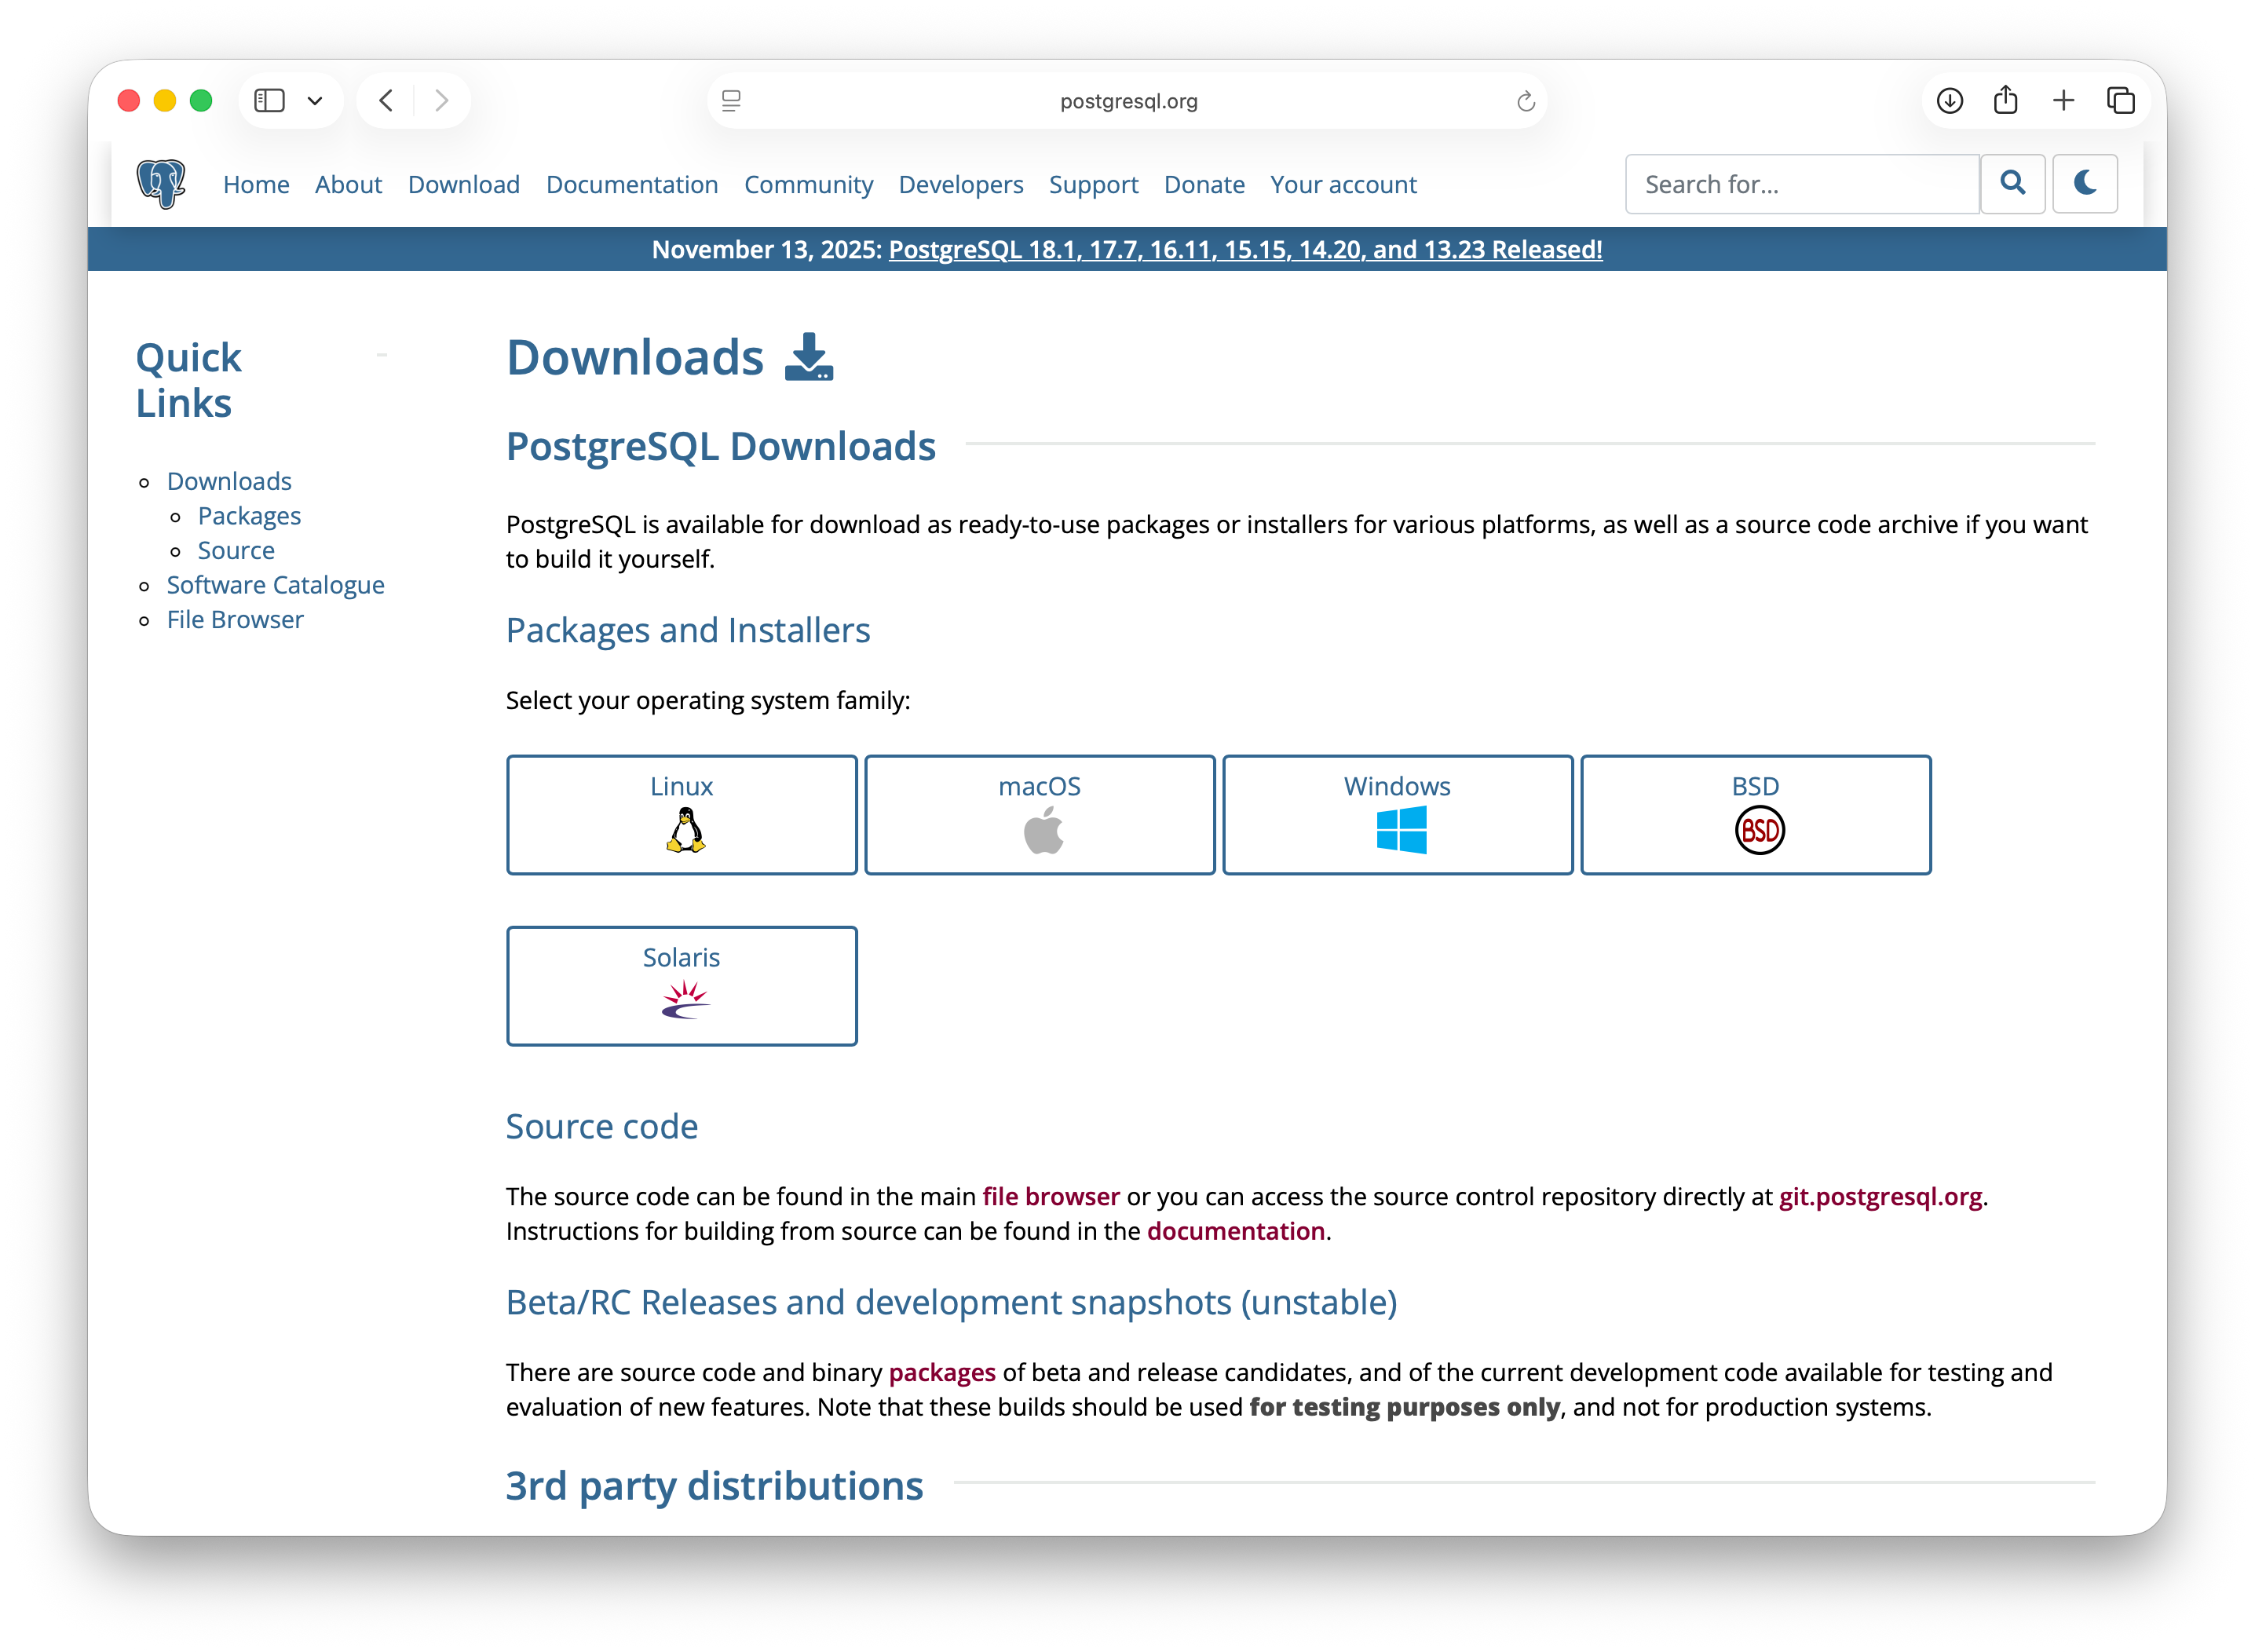
\includegraphics[width=.85\textwidth]{screen60.png}
\end{center}

\clearpage
\item Select the MacOS download for the latest version of PostgreSQL.

\begin{center}
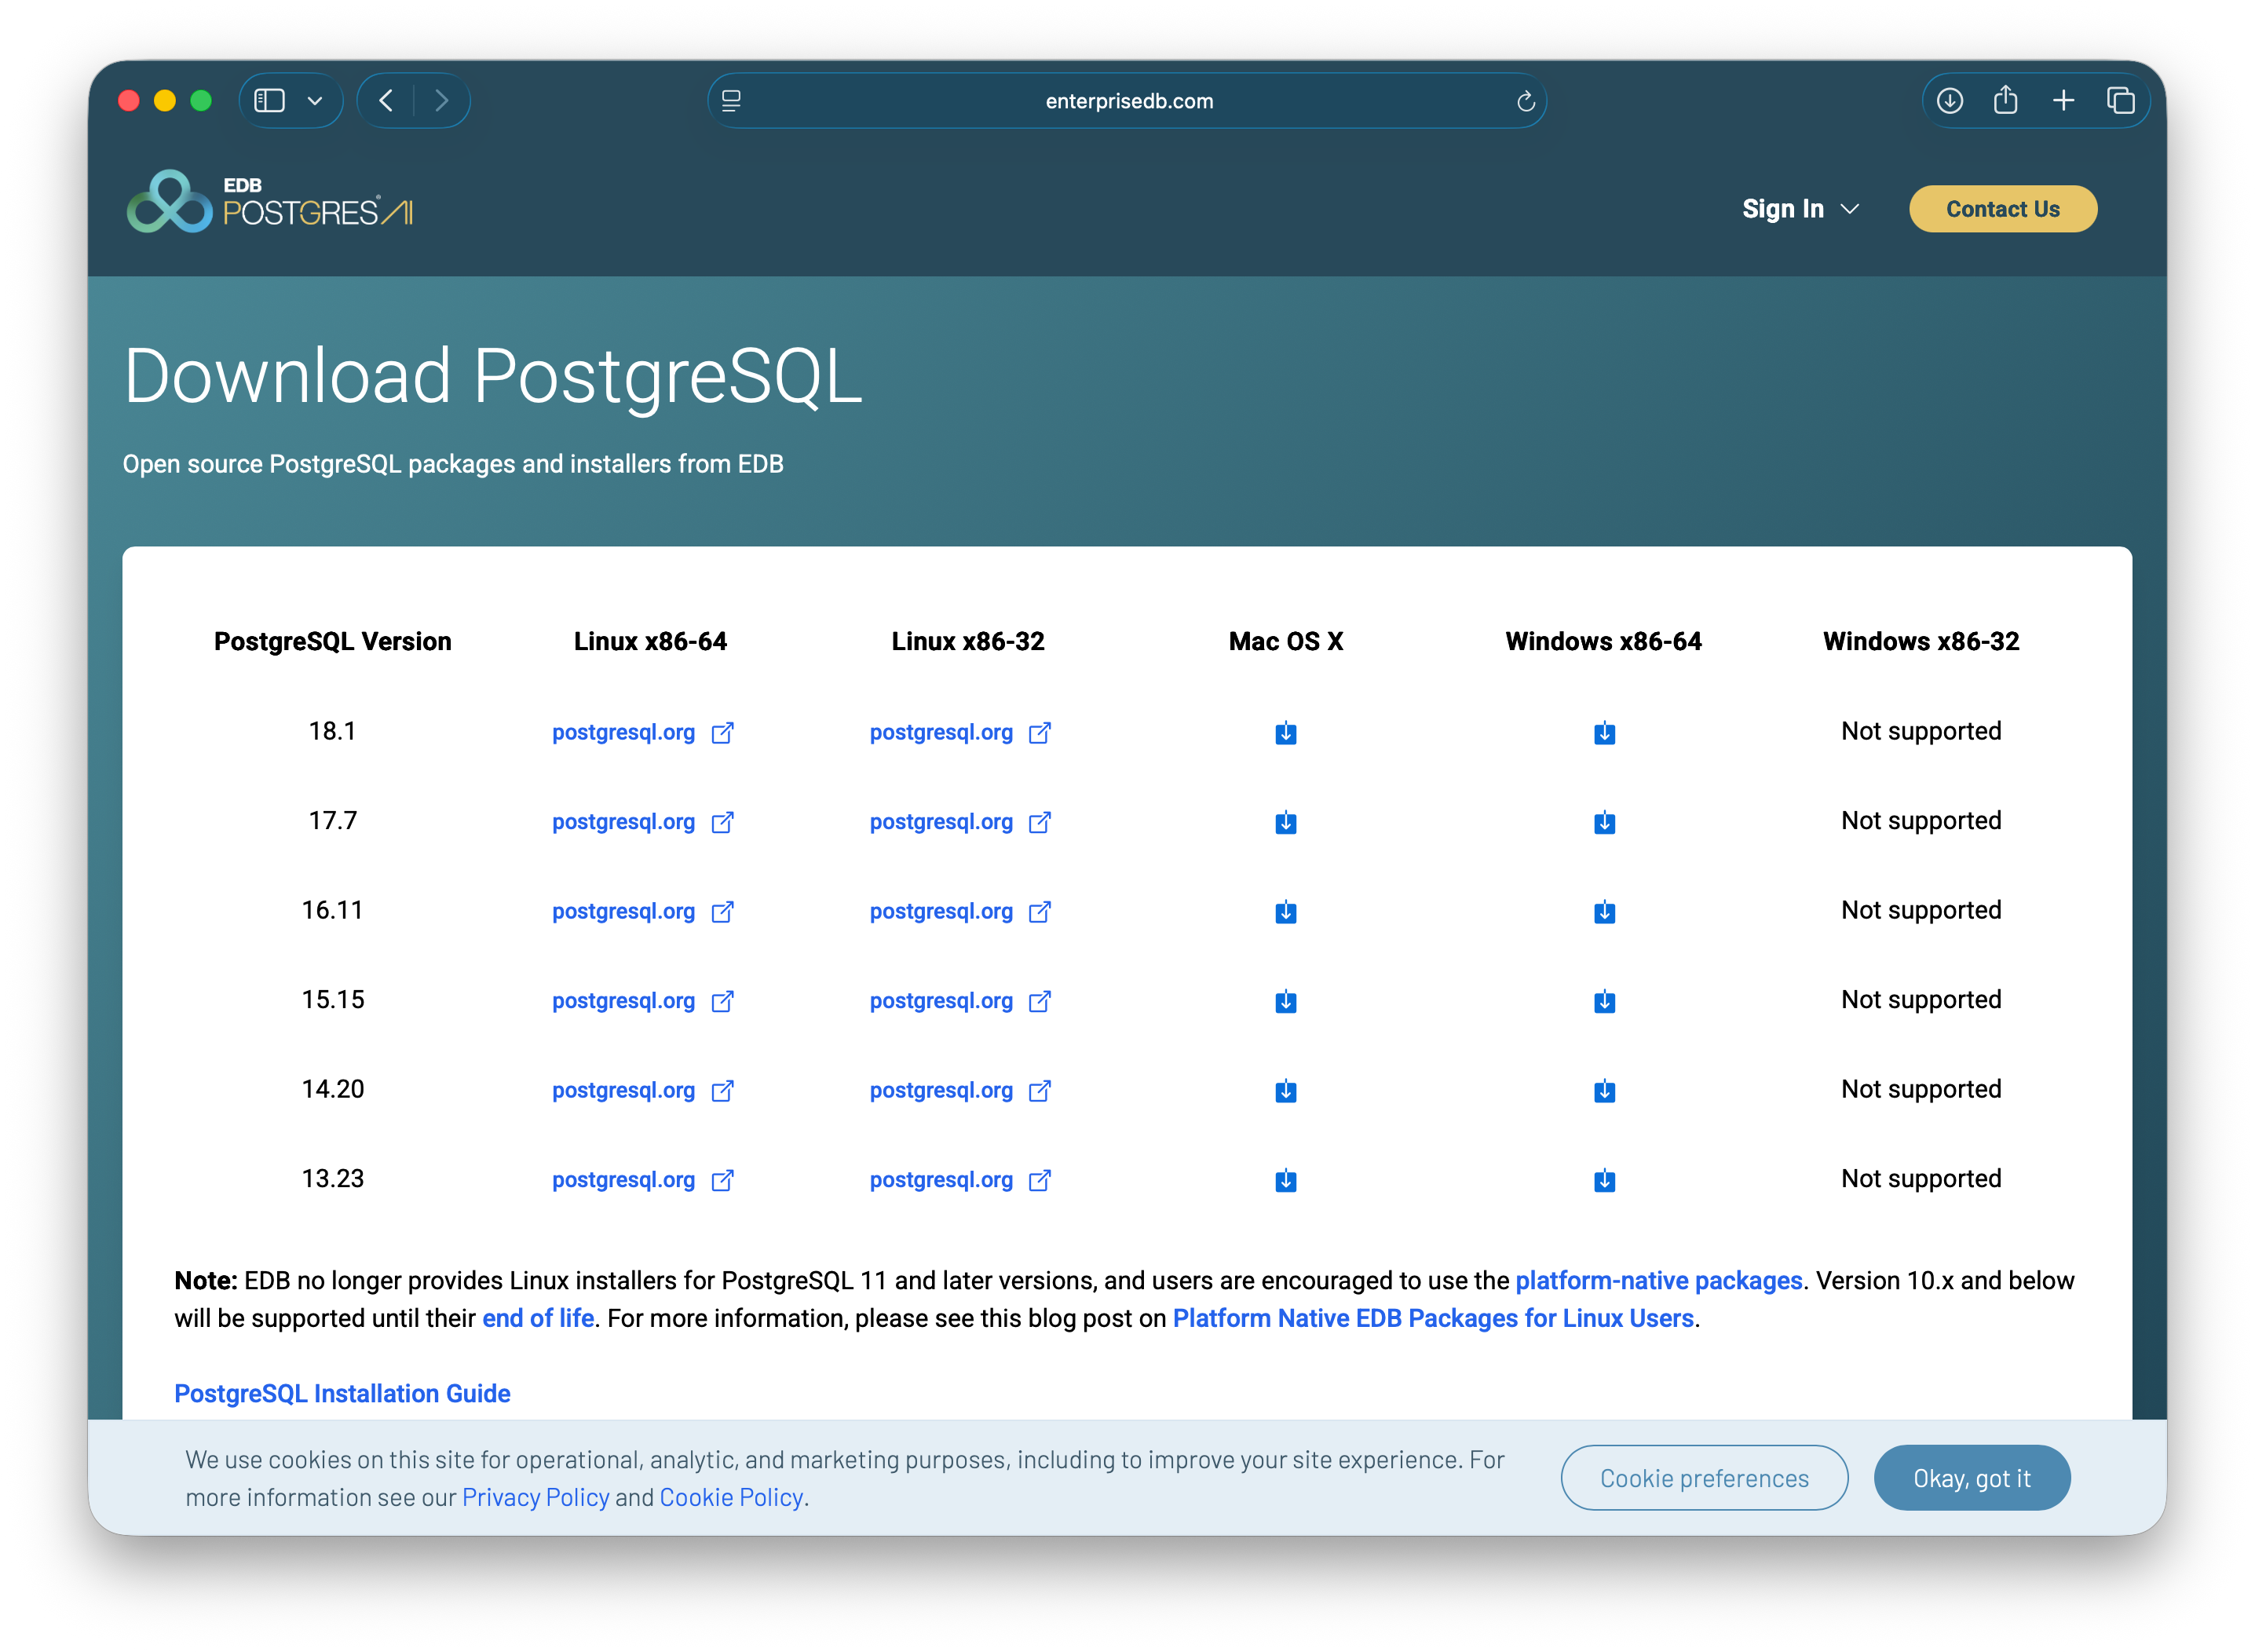
\includegraphics[width=.85\textwidth]{screen61.png}
\end{center}

\item Once the download is completed, open the downloaded file. You will see a Folder window containing the installer application for PostgreSQL.

\begin{center}
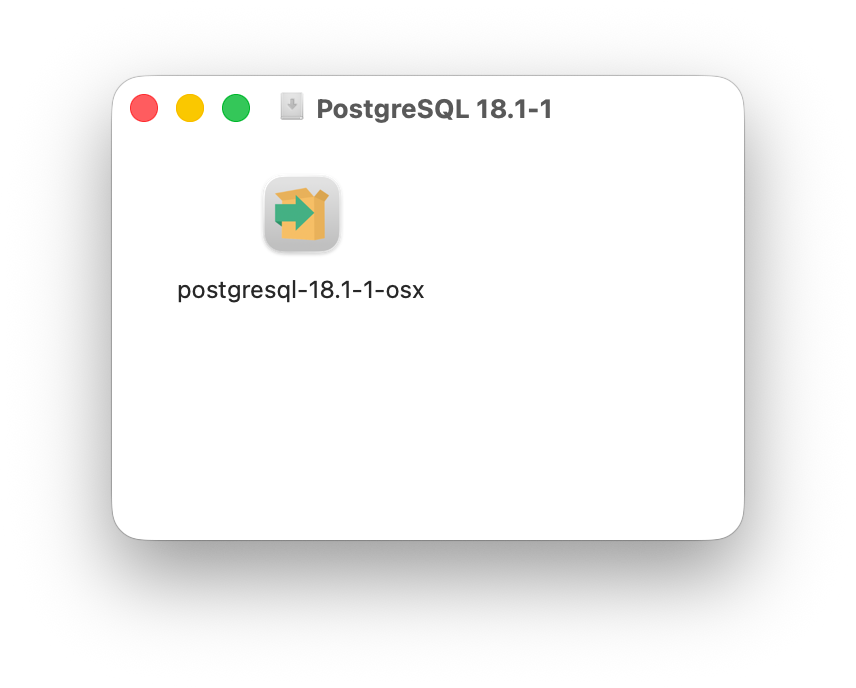
\includegraphics[width=.65\textwidth]{screen62.png}
\end{center}

\clearpage
\item Doubleclick to launch the PostgreSQL installer app. 

\begin{center}
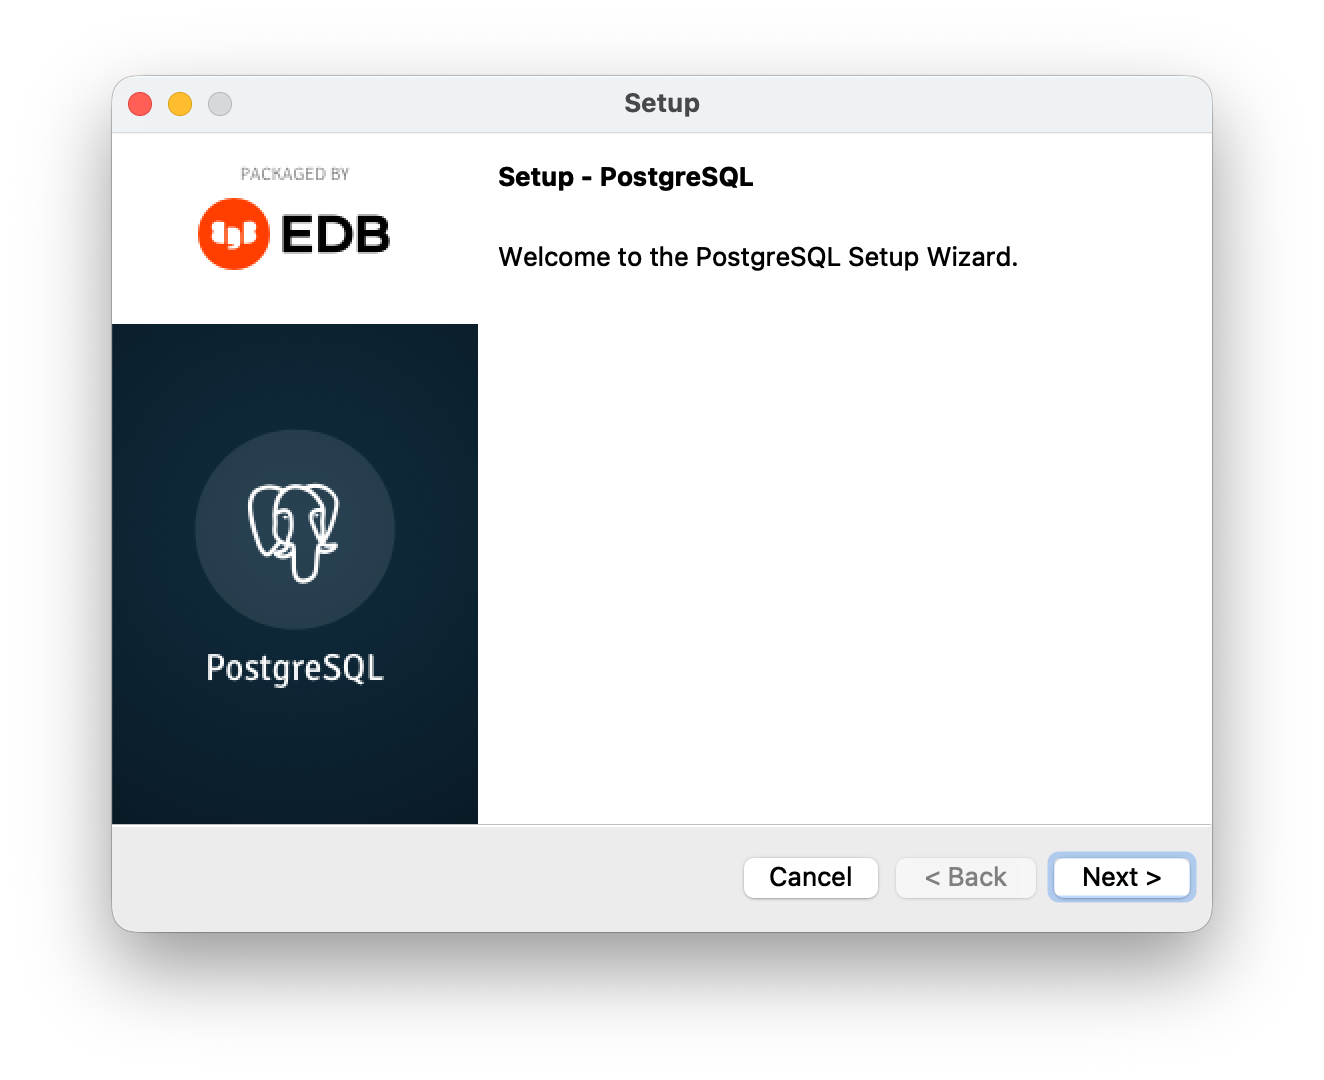
\includegraphics[width=.95\textwidth]{screen63.png}
\end{center}

\item Click the ''Next'' button on each installer dialog window. You do not need to change any of the values or options.

\item You will be asked to enter a password for the super user of the database system. Enter a password that you will remember, as you will need it later.

\begin{center}
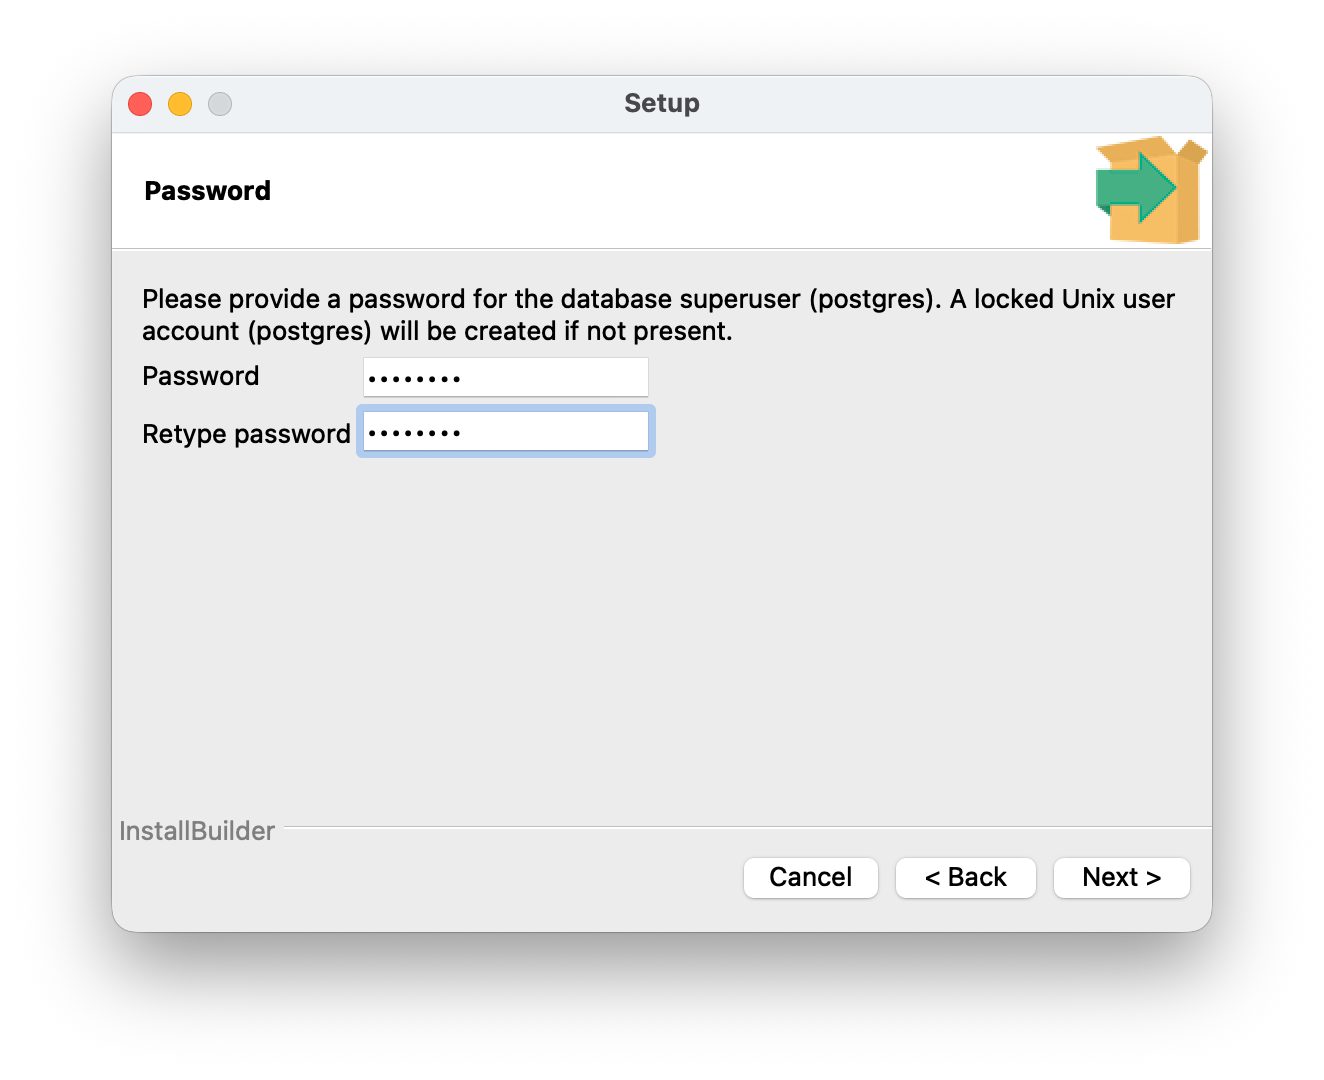
\includegraphics[width=.95\textwidth]{screen64.png}
\end{center}

Continue with the installation by clicking the ''Next'' button on each installer dialog window.

\clearpage
\item Once the installation is finished, you do need to launch Stack Builder. Unselect the tick box, then click the ''Finish'' button.

\begin{center}
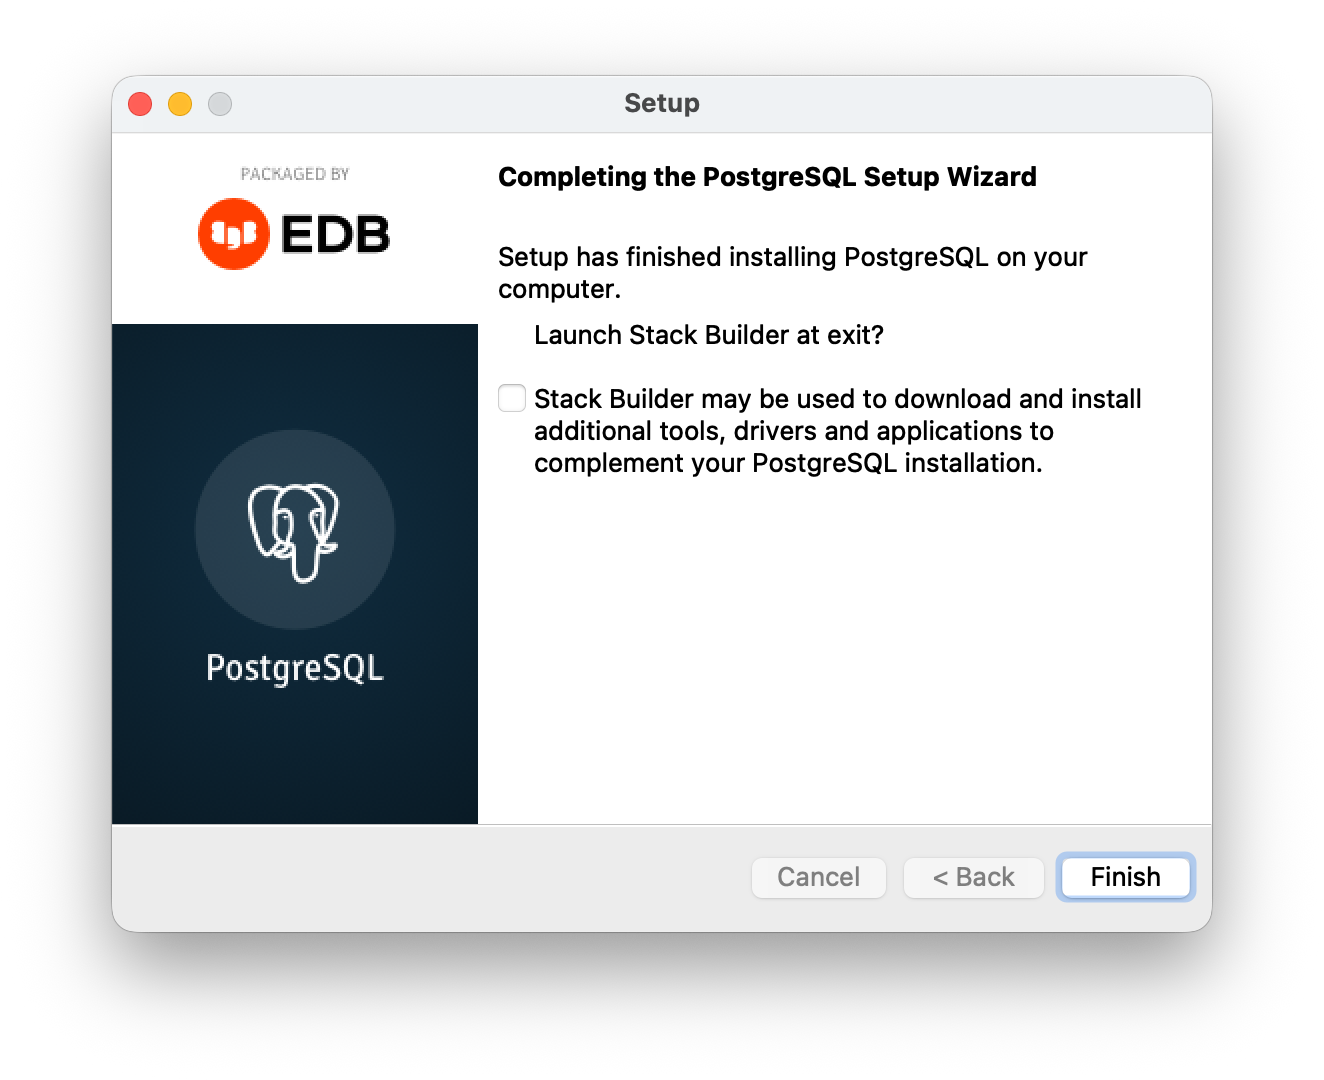
\includegraphics[width=.95\textwidth]{screen65.png}
\end{center}

\item Once the installation is complete, you must install pgAdmin to administer, manage, and interact with the PostgreSQL databases. 

\begin{resourcebox}
pgAdmin is a cross-platform database administration tool for PostgreSQL. Besides many in-depth management features, it also provides and easy way to query the database. \\

\url{https://www.pgadmin.org}
\end{resourcebox}

\clearpage
\item Using your web browser, navigate to the pgAdmin web site.

\begin{center}
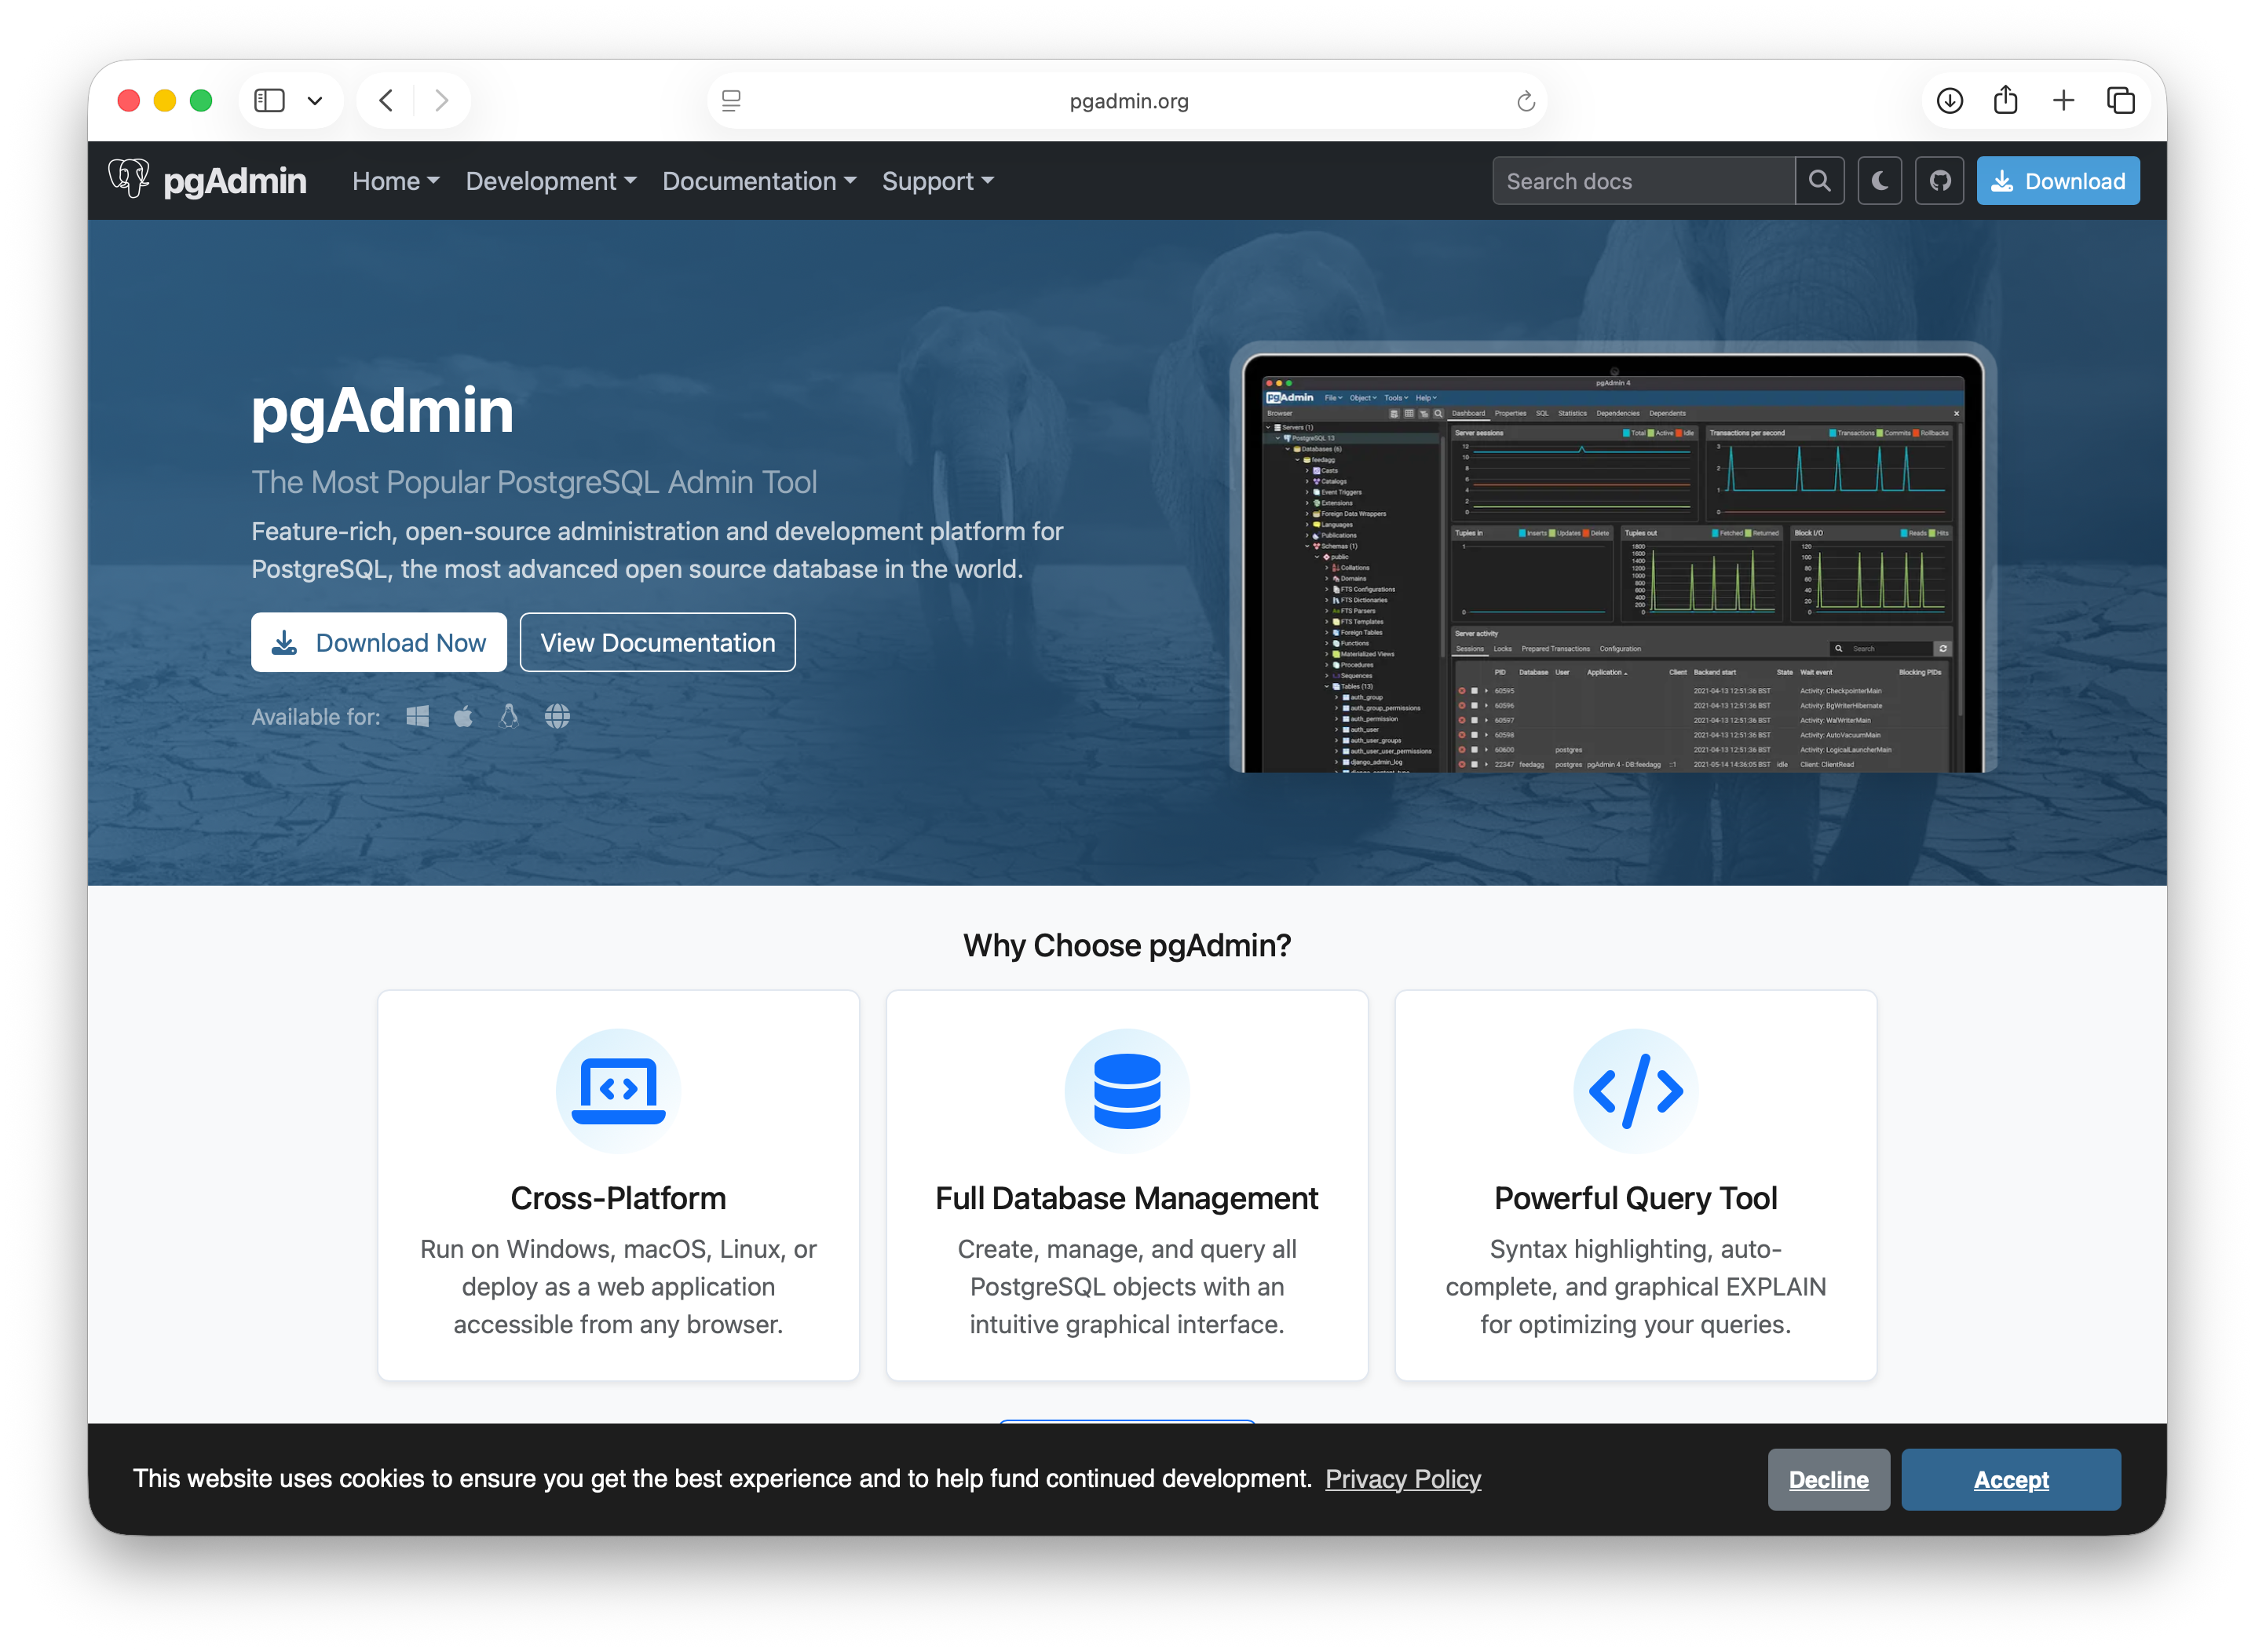
\includegraphics[width=.95\textwidth]{screen66.png}
\end{center}

\item Navigate to the download page, then choose ''macOS''.

\begin{center}
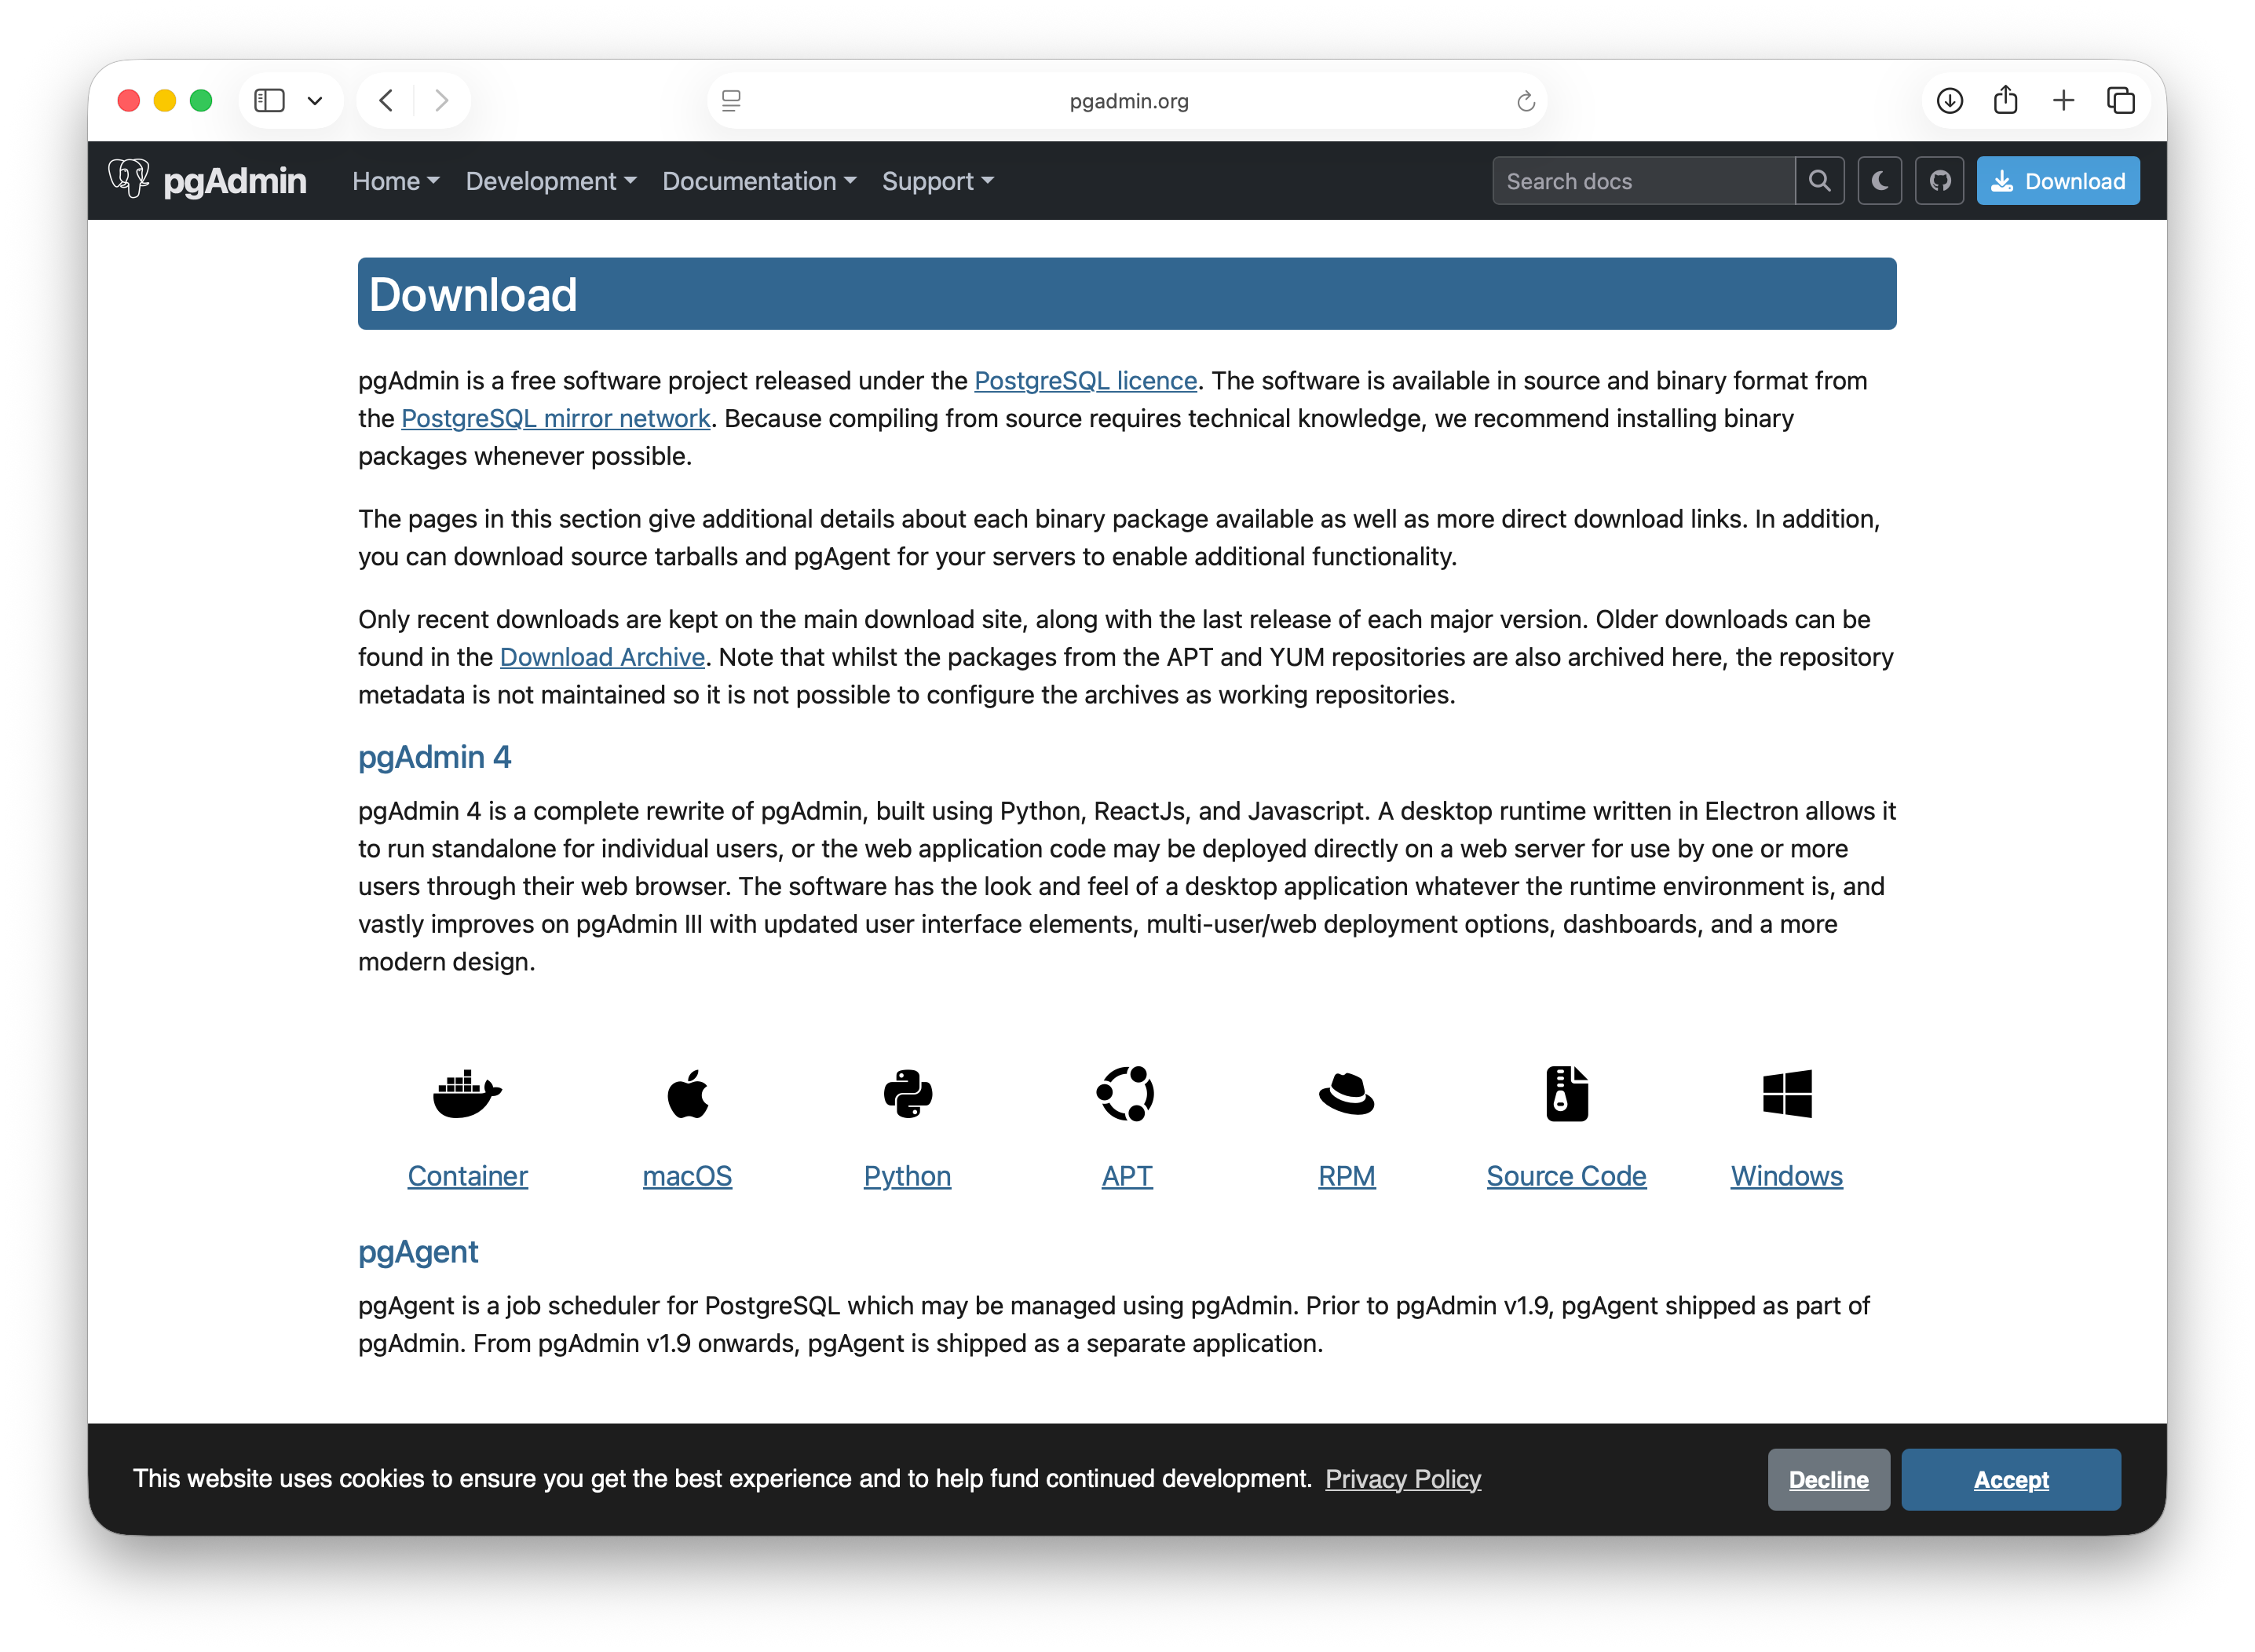
\includegraphics[width=.95\textwidth]{screen67.png}
\end{center}

\clearpage
\item On the following web page, select the latest version of pgAdmin for download.

\begin{center}
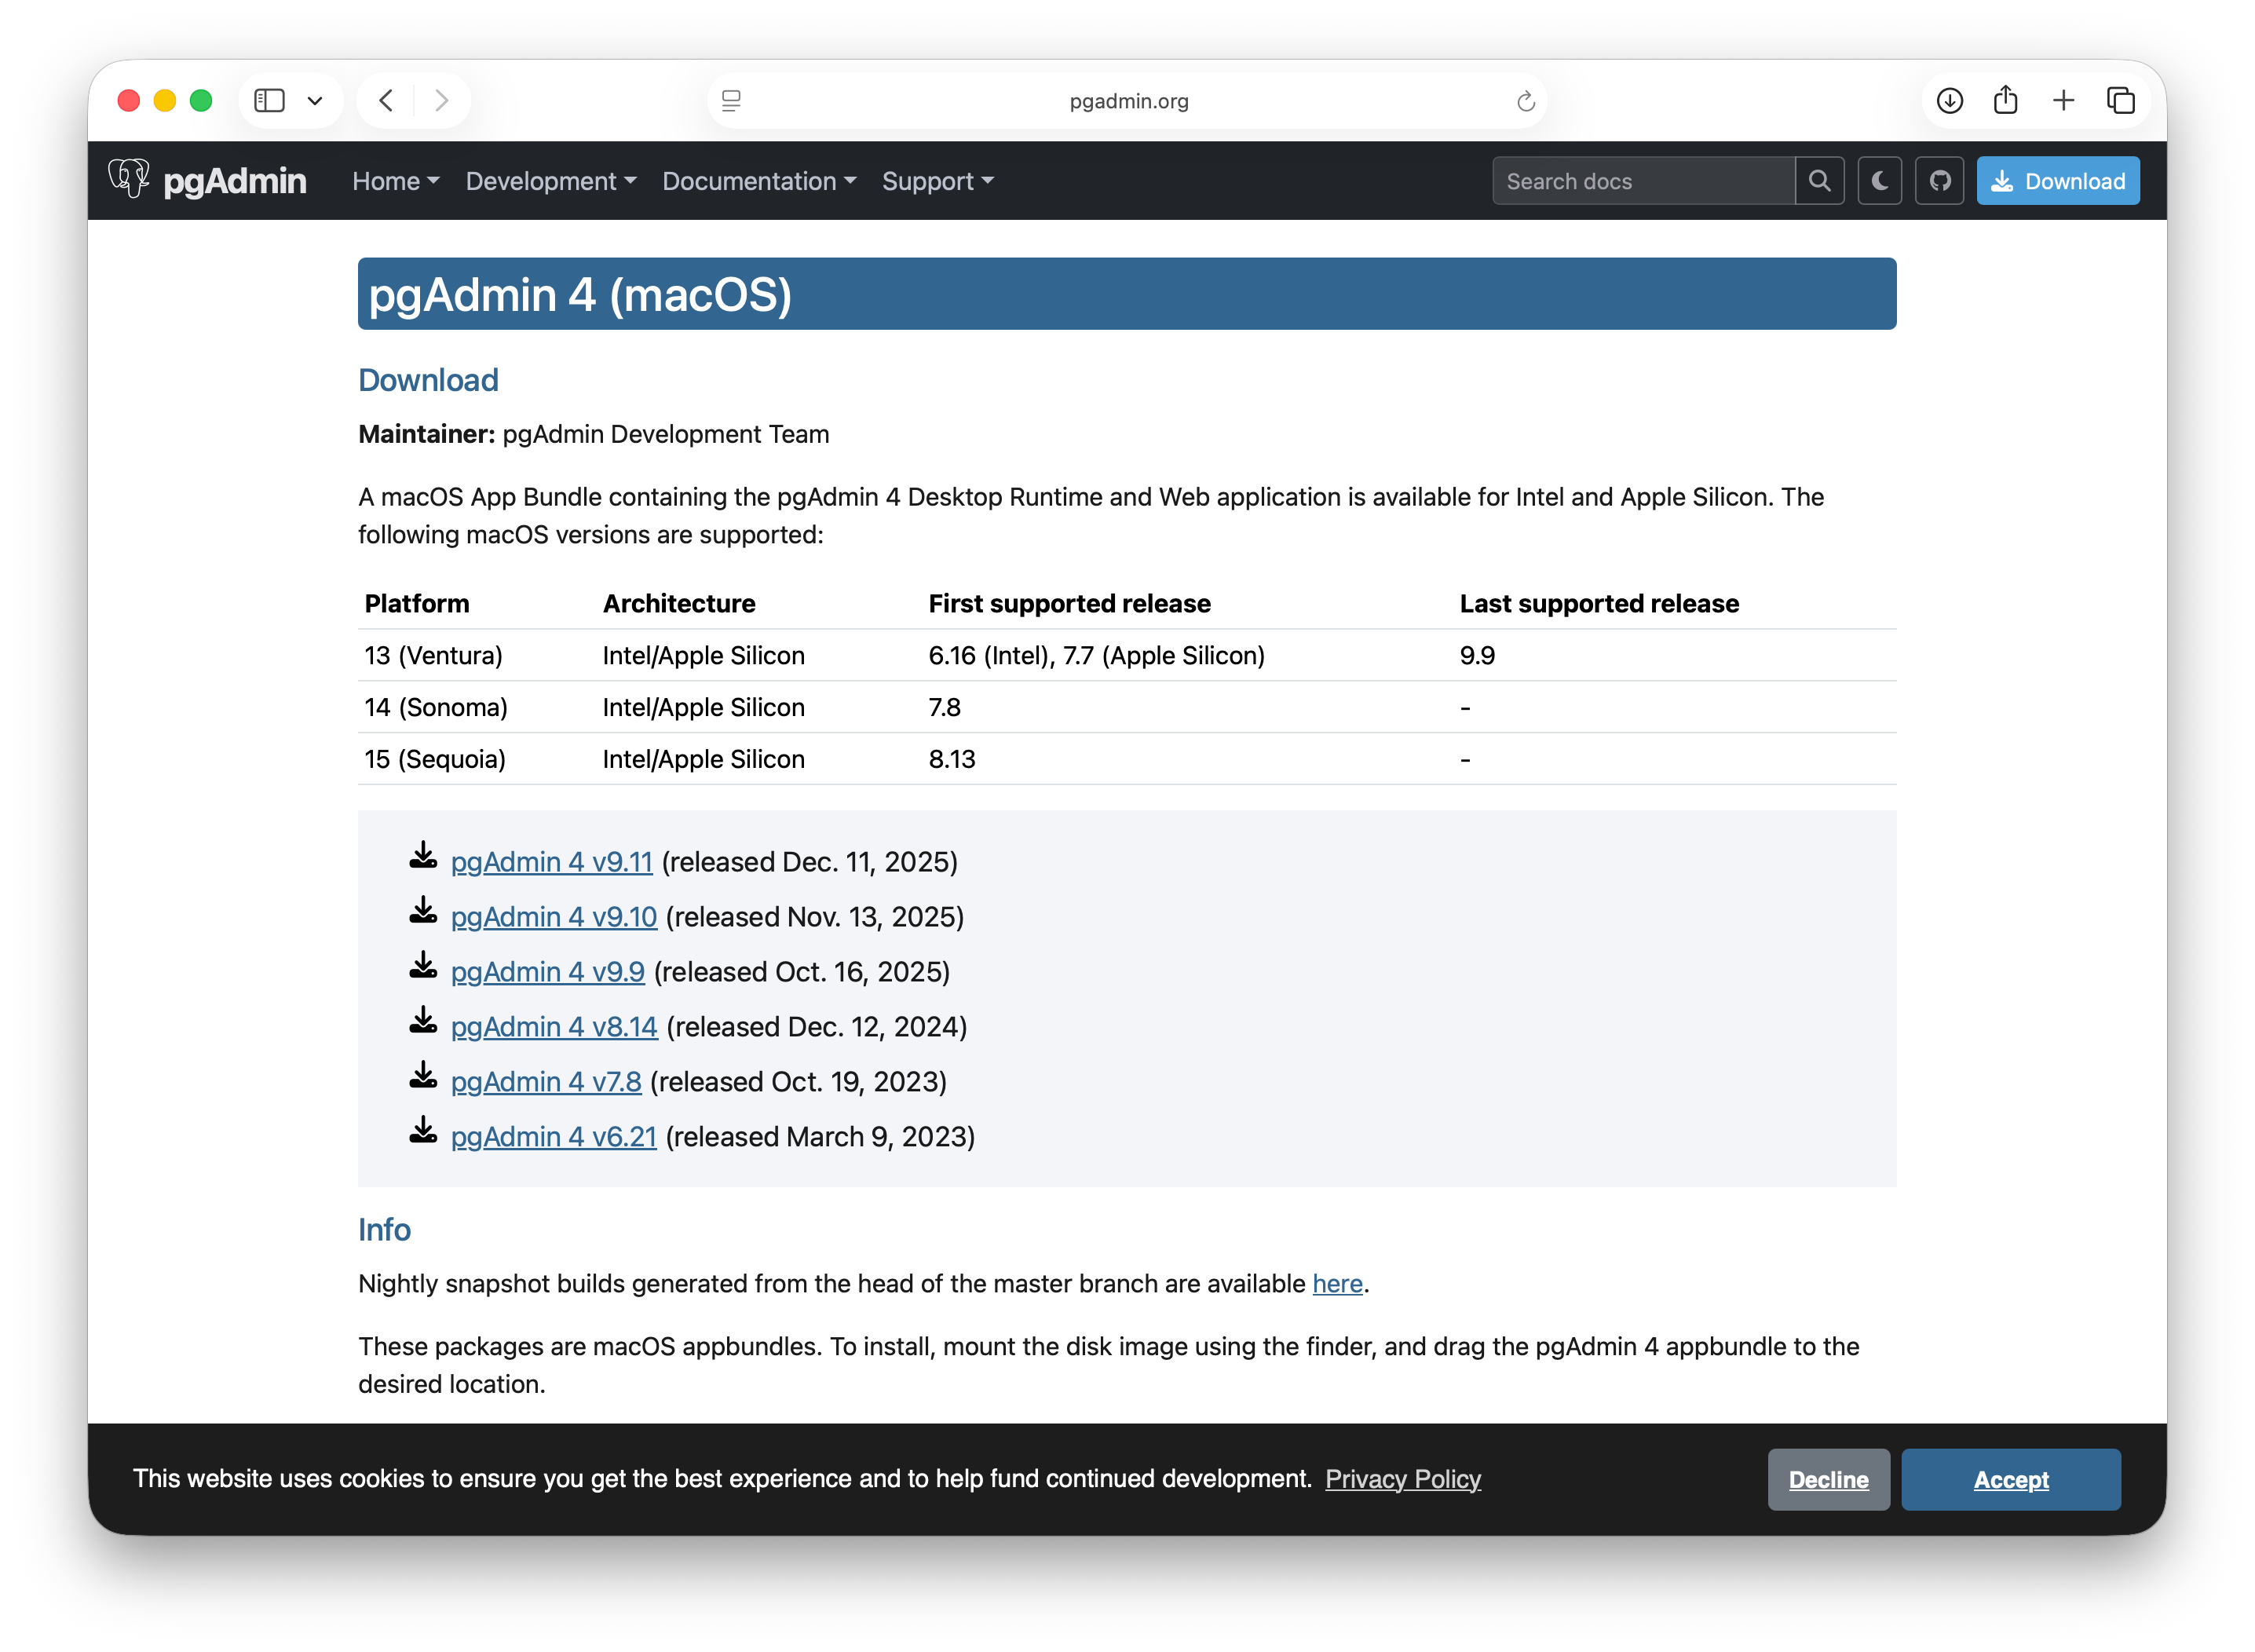
\includegraphics[width=.95\textwidth]{screen68.png}
\end{center}

\item Then, select the appropriate version. For Apple silicon computers (M1, M2, etc., approx. since 2021), choose the ''arm64'' version, for older Intel Mac computers, choose the ''x64'' version.

\begin{center}
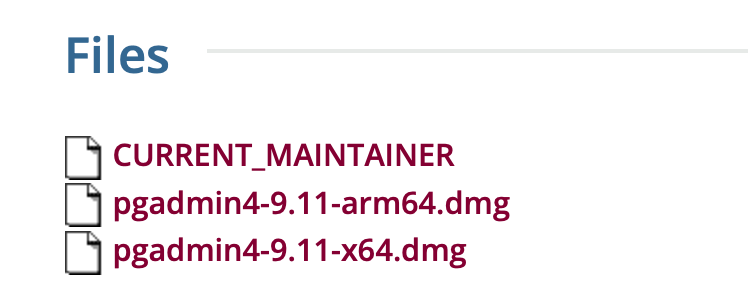
\includegraphics[width=.55\textwidth]{screen69.png}
\end{center}

\clearpage
\item Once the download has finished, click on the downloaded file to begin the installation. You must agree to the software license. 

\begin{center}
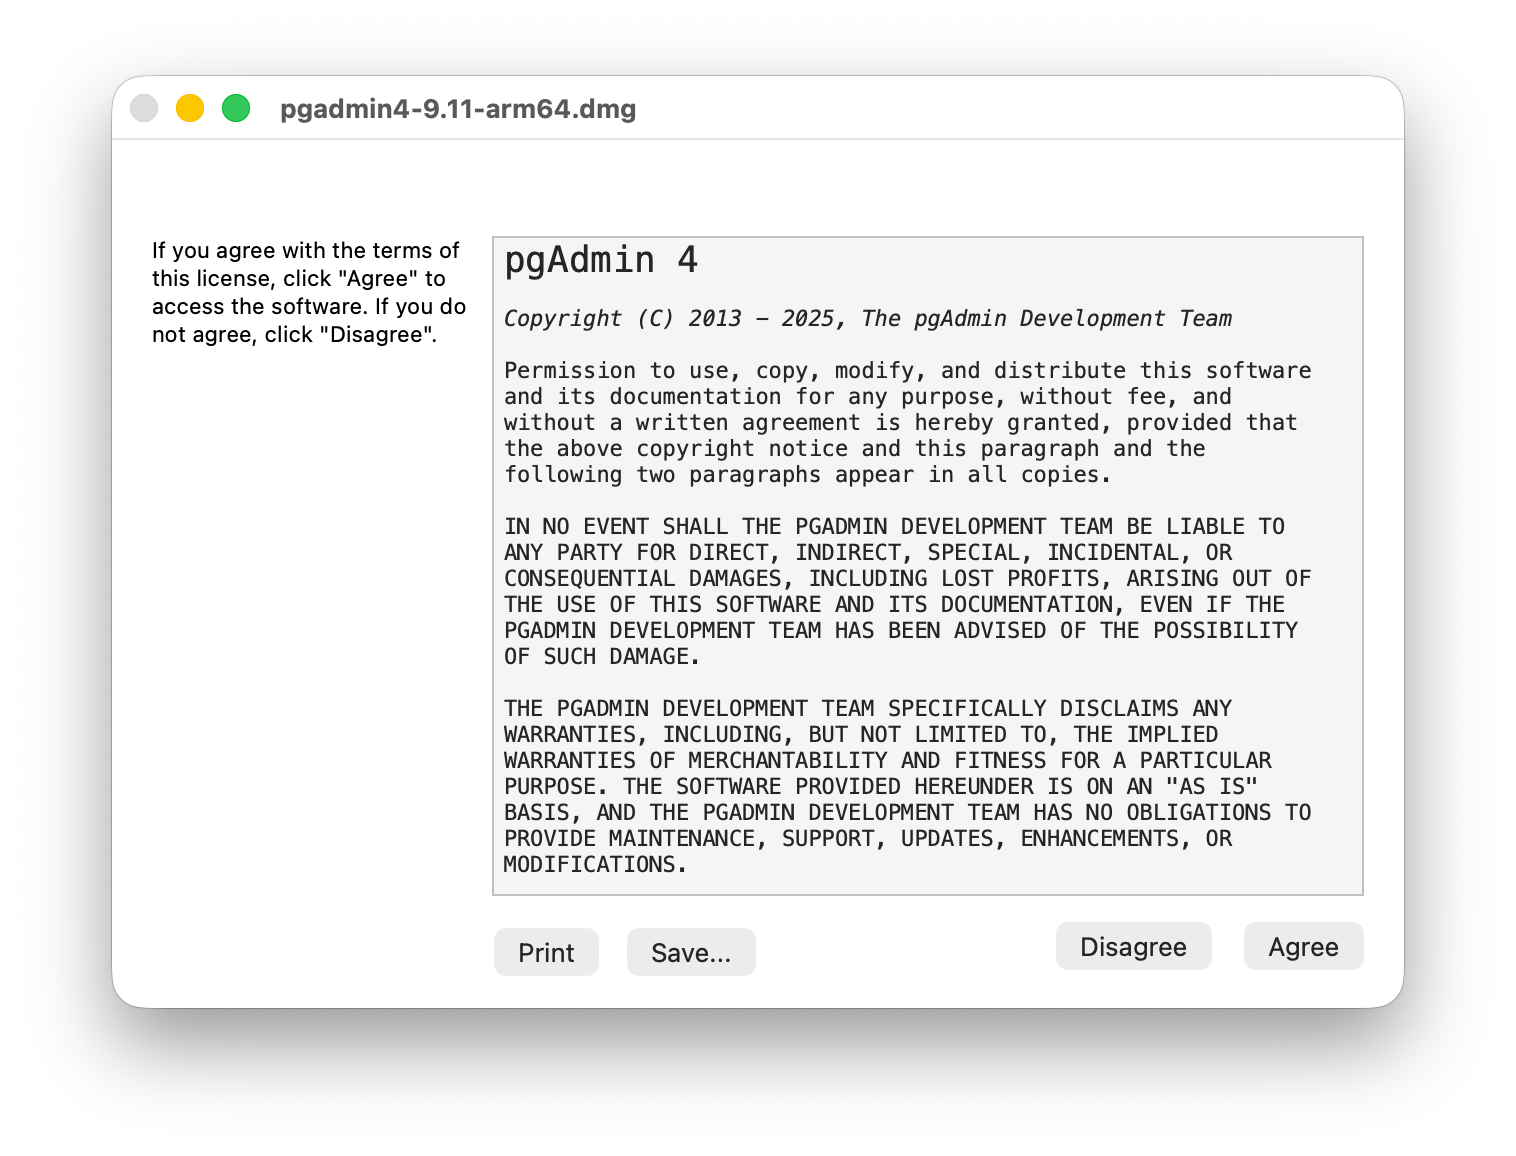
\includegraphics[width=.95\textwidth]{screen70.png}
\end{center}

\item Next, in the pgAdmin window that opens after you agree to the software license, drag and drop the pgAdmin 4 icon in that window to the Applications folder in that window. 

\begin{center}
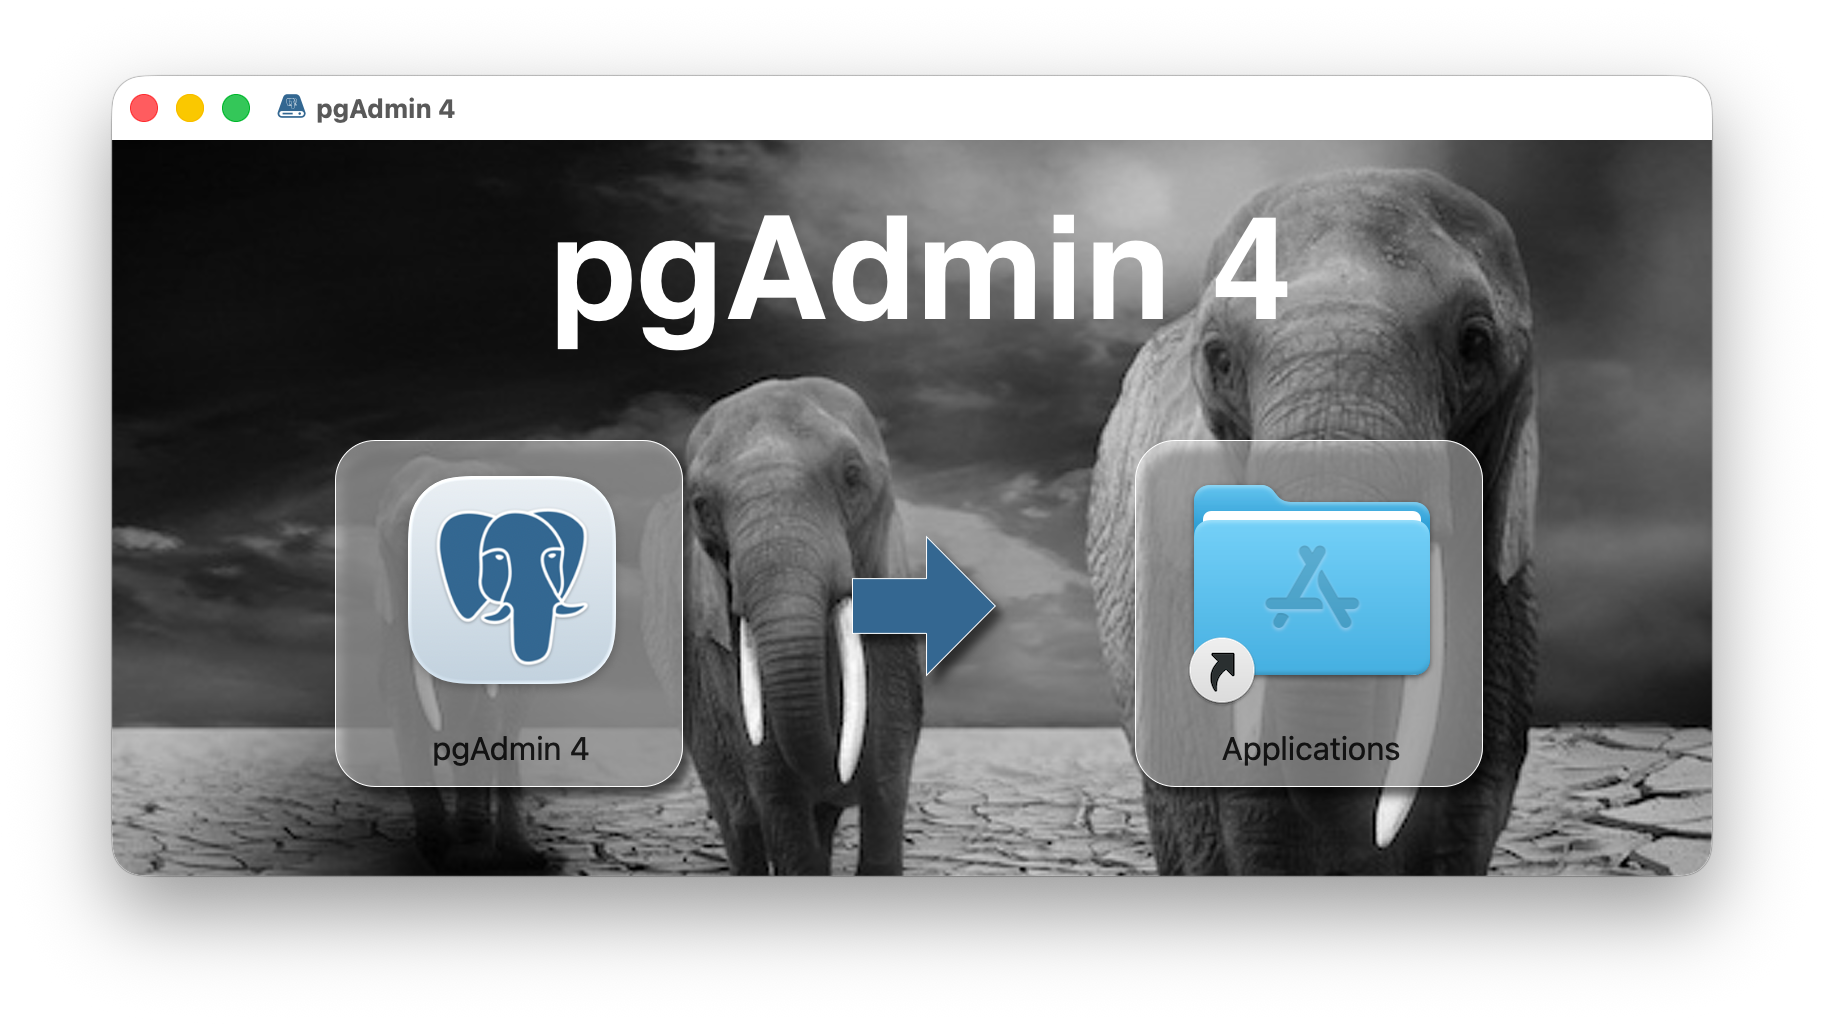
\includegraphics[width=.95\textwidth]{screen71.png}
\end{center}

\clearpage
\item In your Finder, navigate to the Applications folder and select the pgAdmin 4 application. Double-click on it to start pgAdmin.

\begin{center}
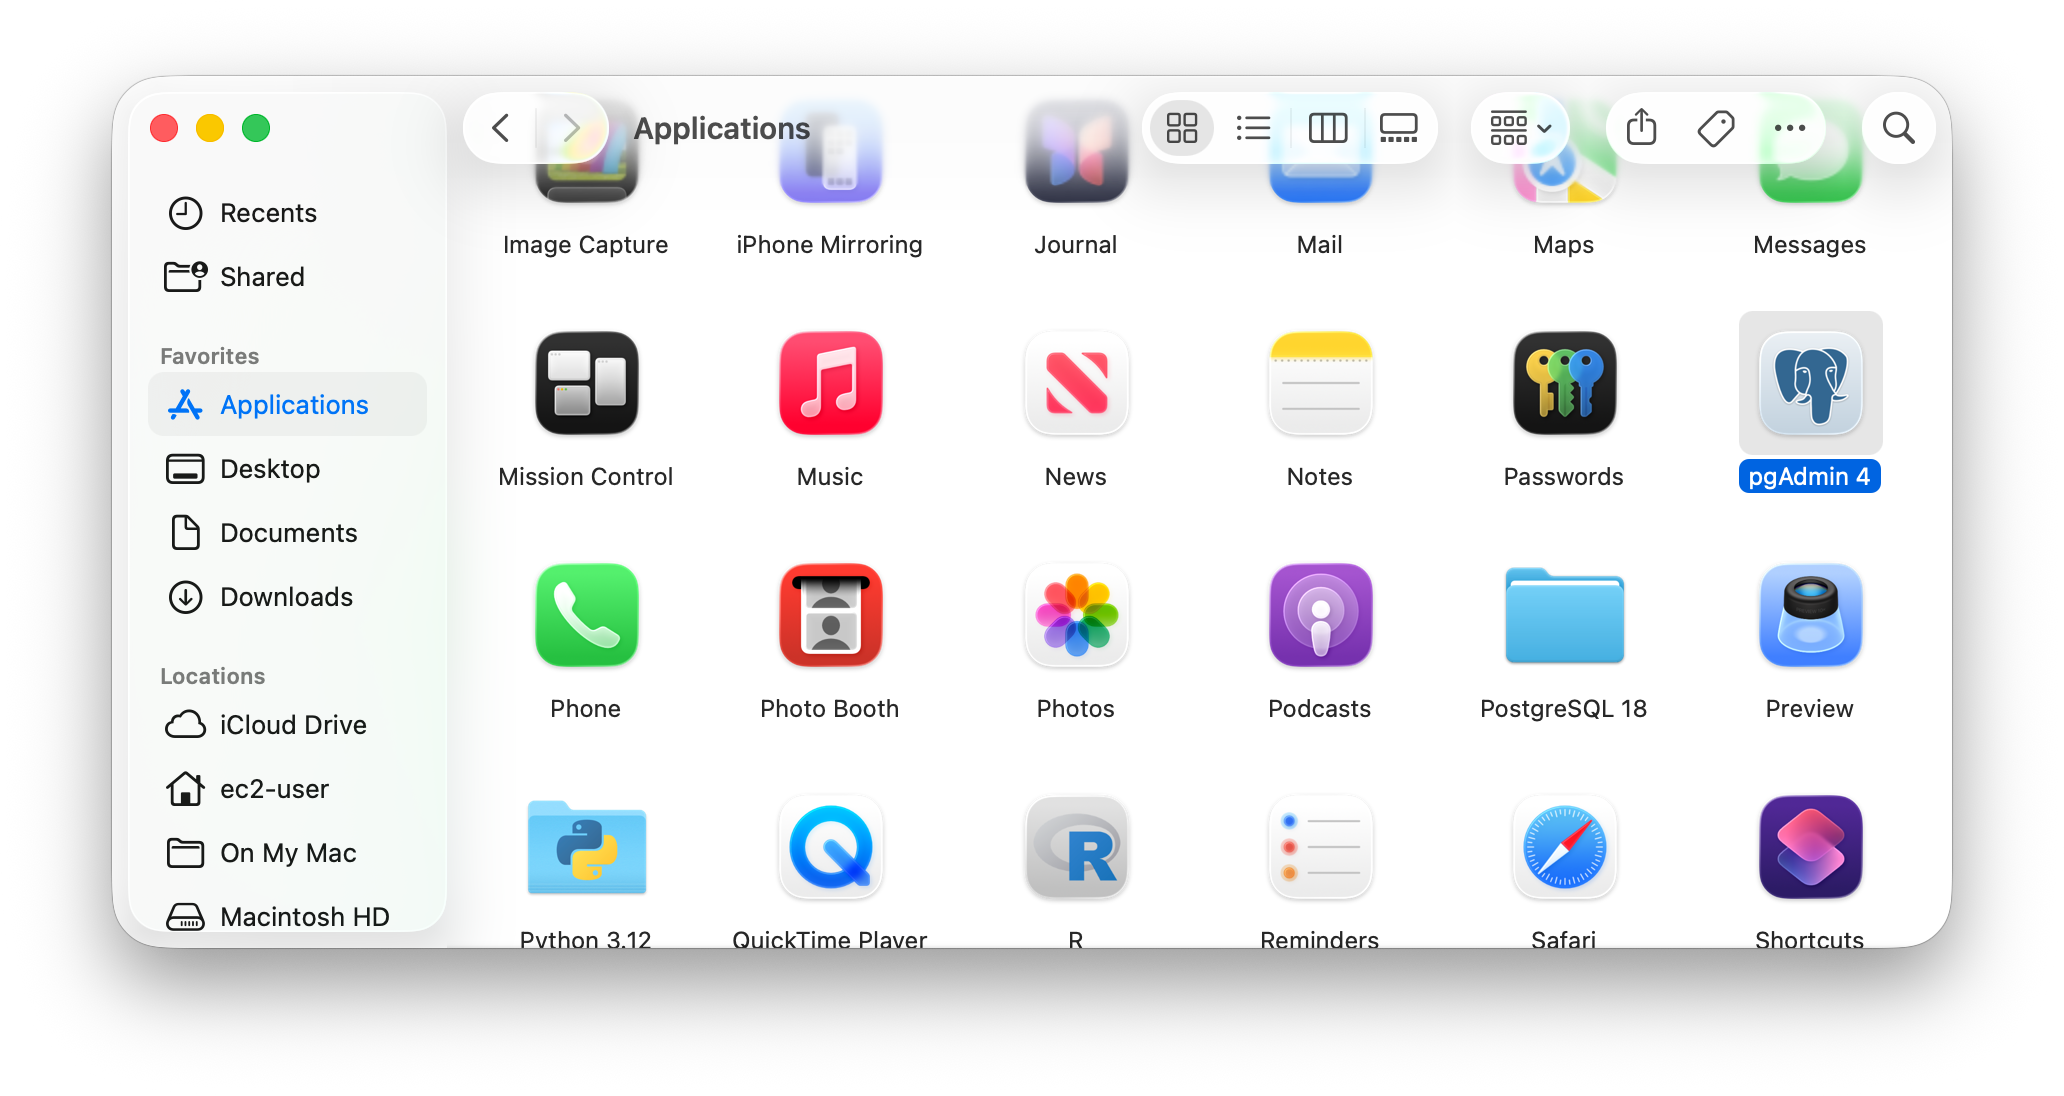
\includegraphics[width=.95\textwidth]{screen72.png}
\end{center}

You will be asked to permit local network access for pgAdmin. You must allow this.

\begin{center}
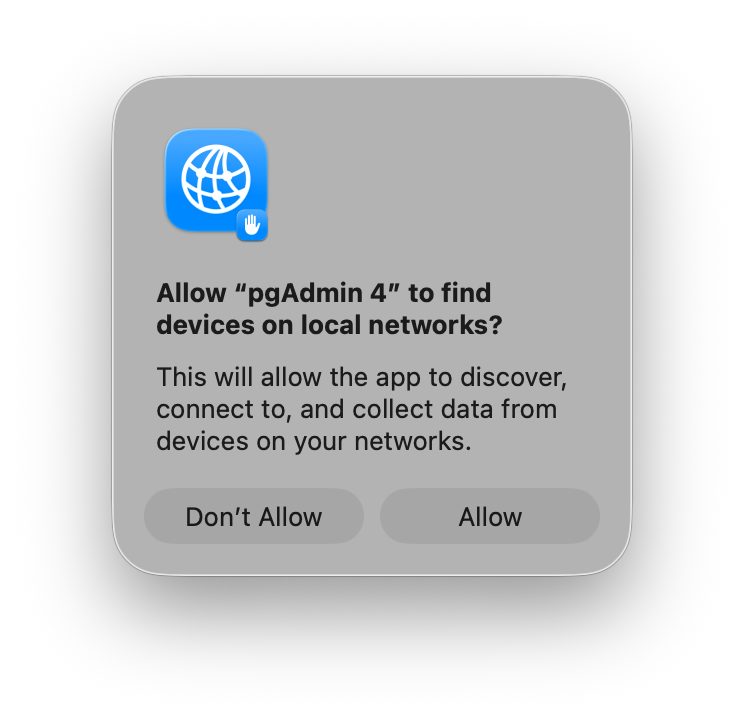
\includegraphics[width=.55\textwidth]{screen73.png}
\end{center}

\clearpage
\item In the pgAdmin app, in the left-hand object browser, navigate to the PostgreSQL entry under the ''Servers'' entry. You will be asked to enter the password that you created earlier during installation of PostgreSQL.

\begin{center}
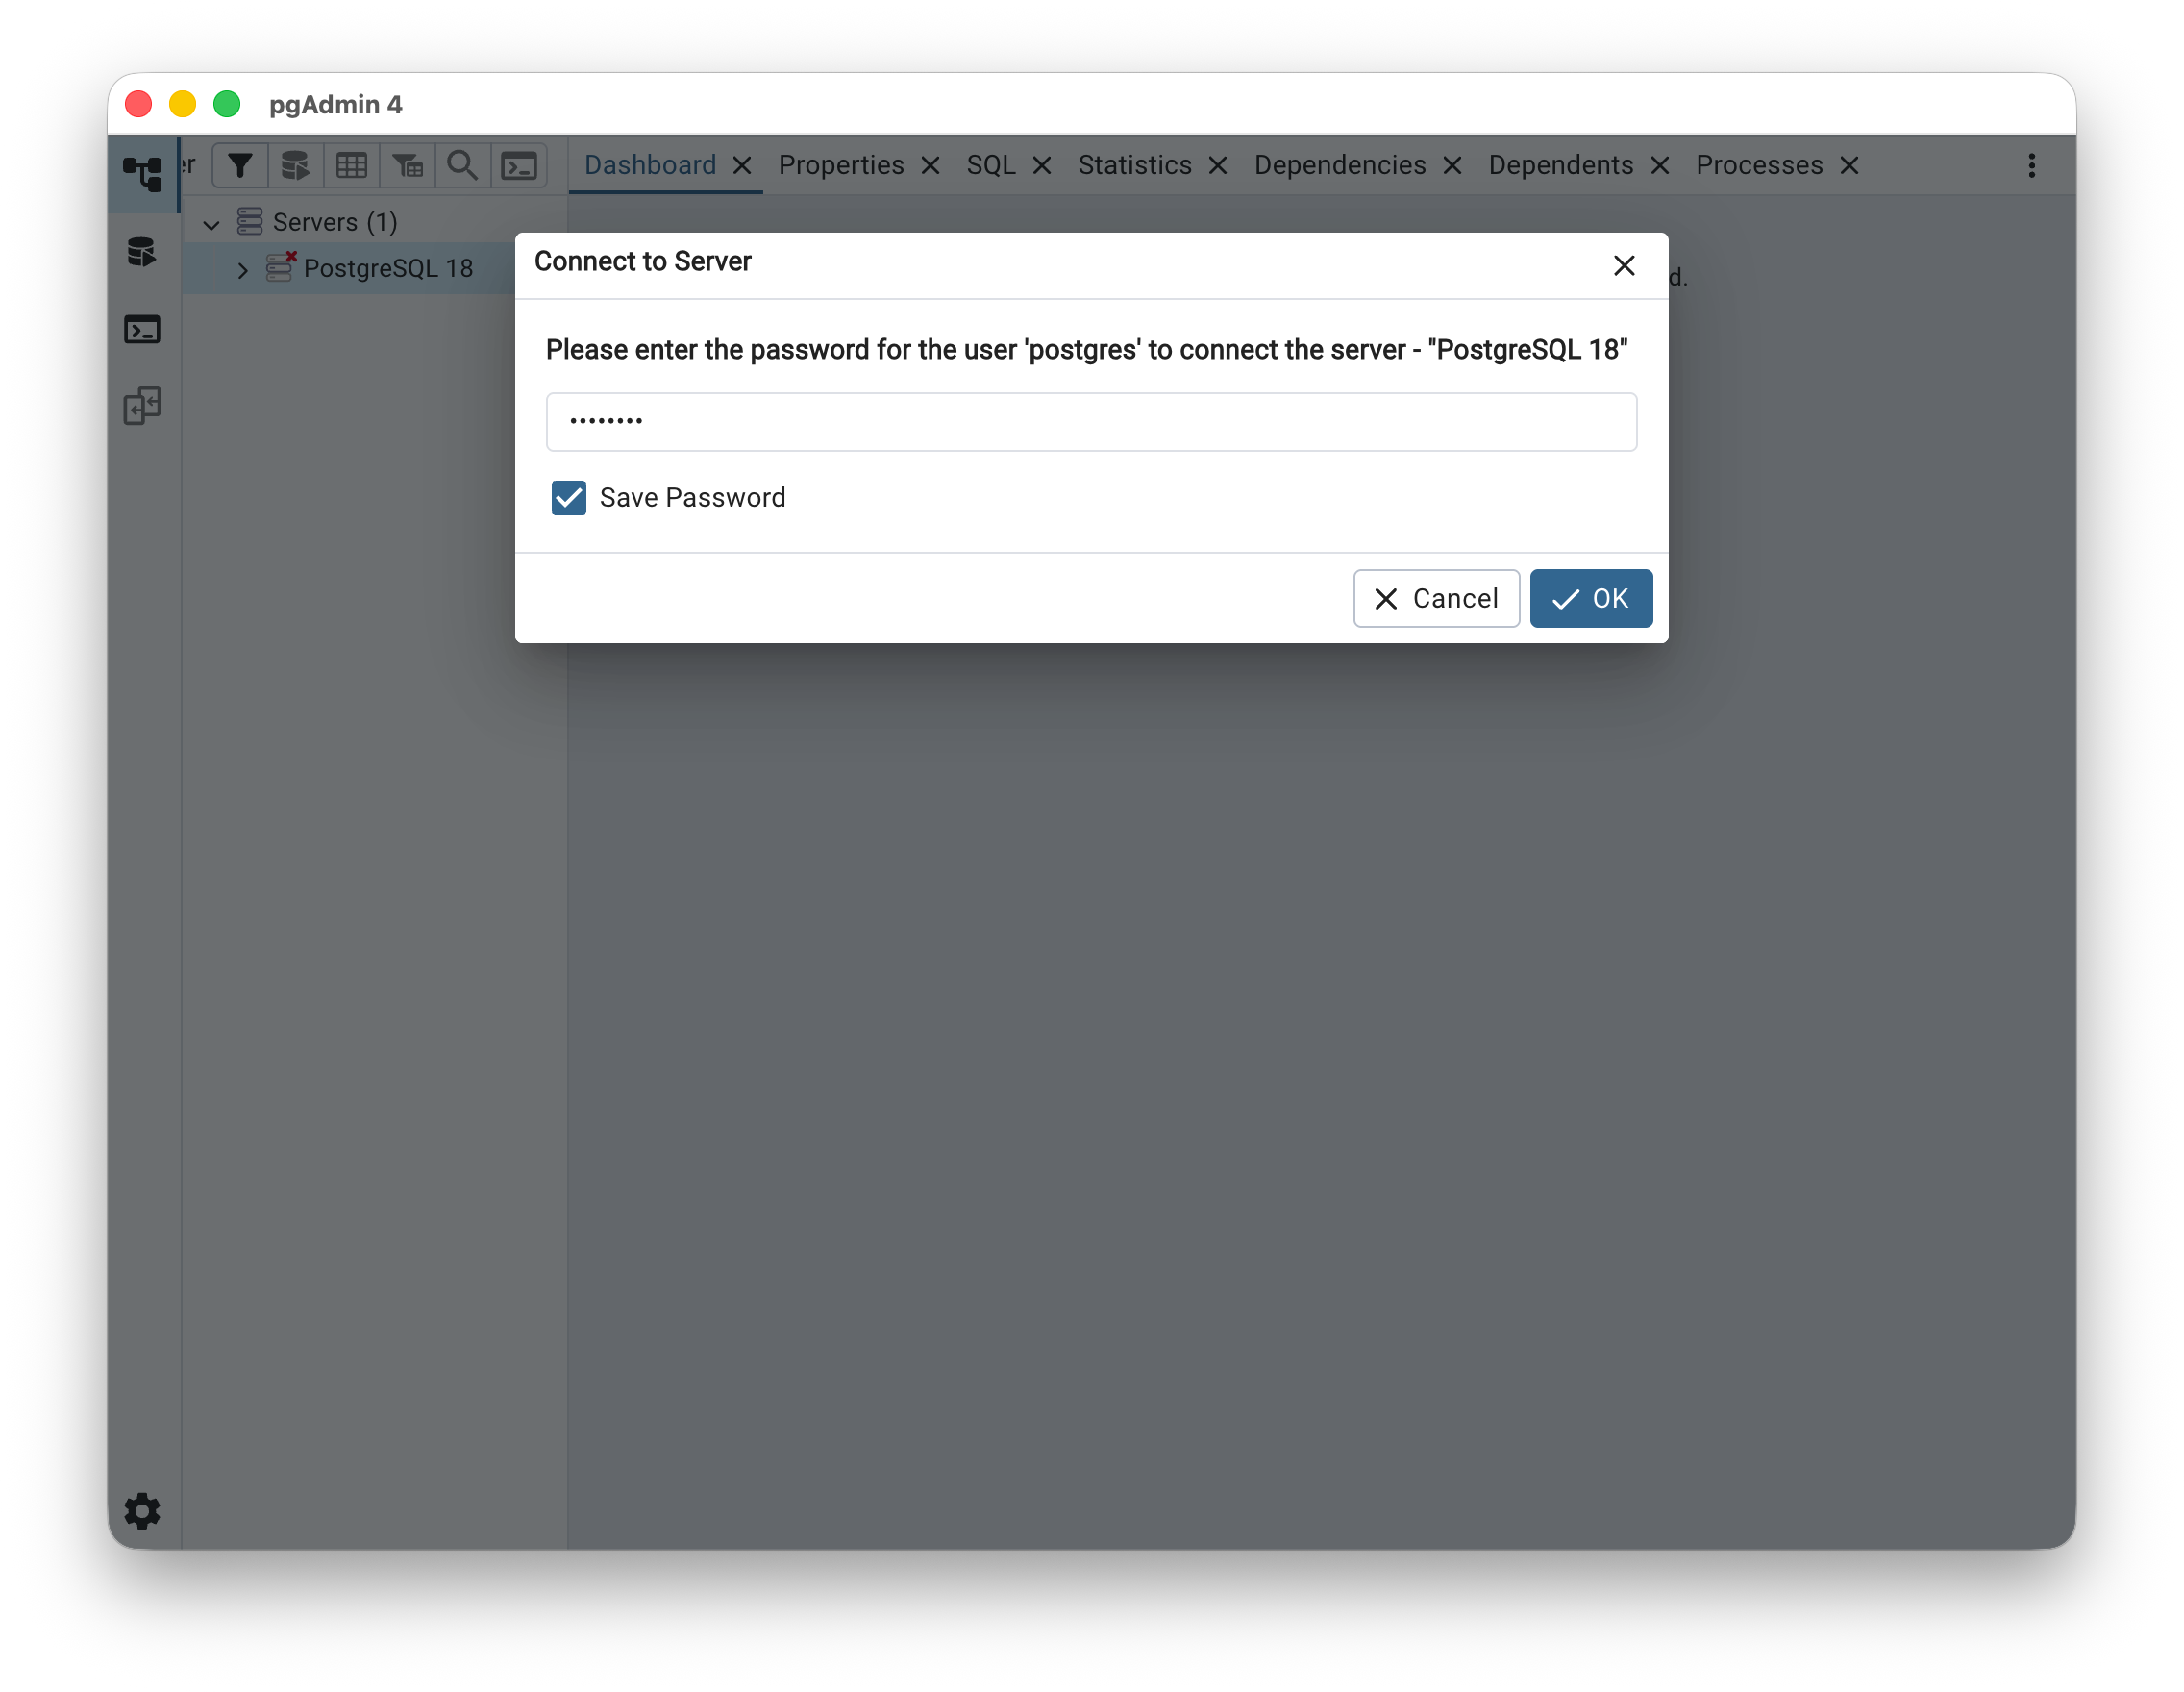
\includegraphics[width=.85\textwidth]{screen74.png}
\end{center}

\item After entering the password, you will see the pgAdmin dashboard.

\begin{center}
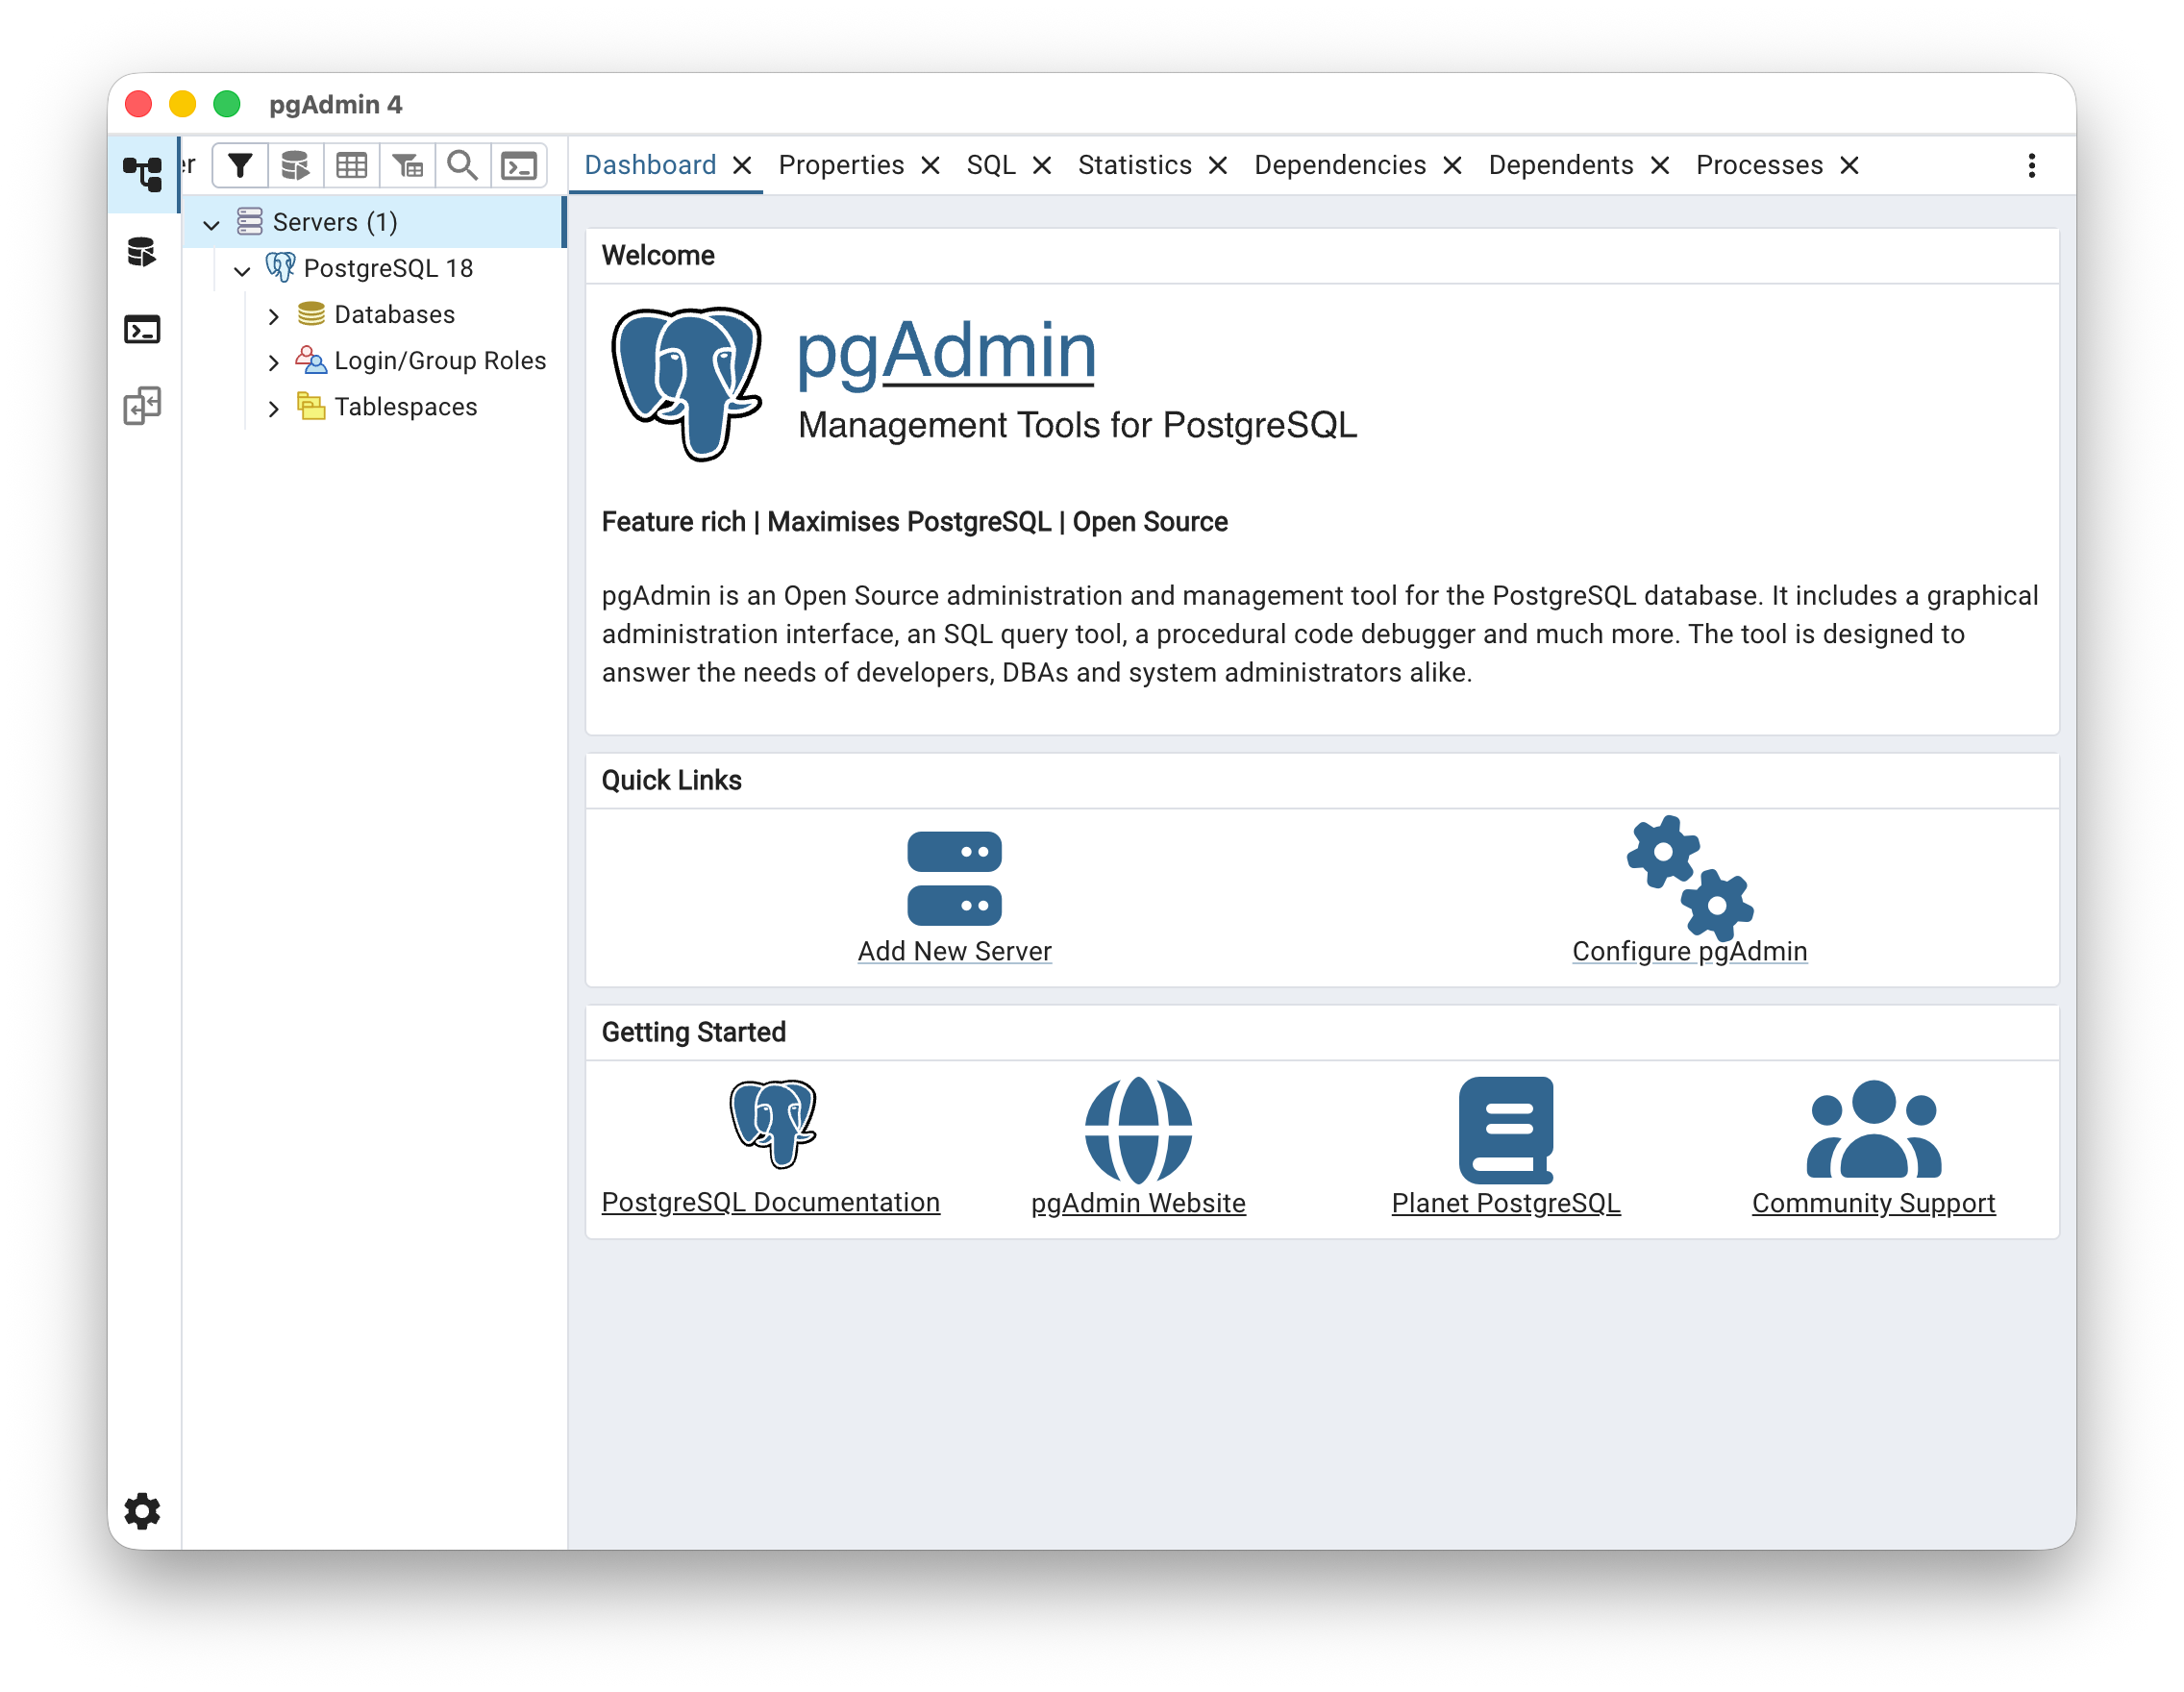
\includegraphics[width=.85\textwidth]{screen75.png}
\end{center}

\clearpage
\item In the object explorer on the left-hand side, navigate to the ''postgres'' database.

\begin{center}
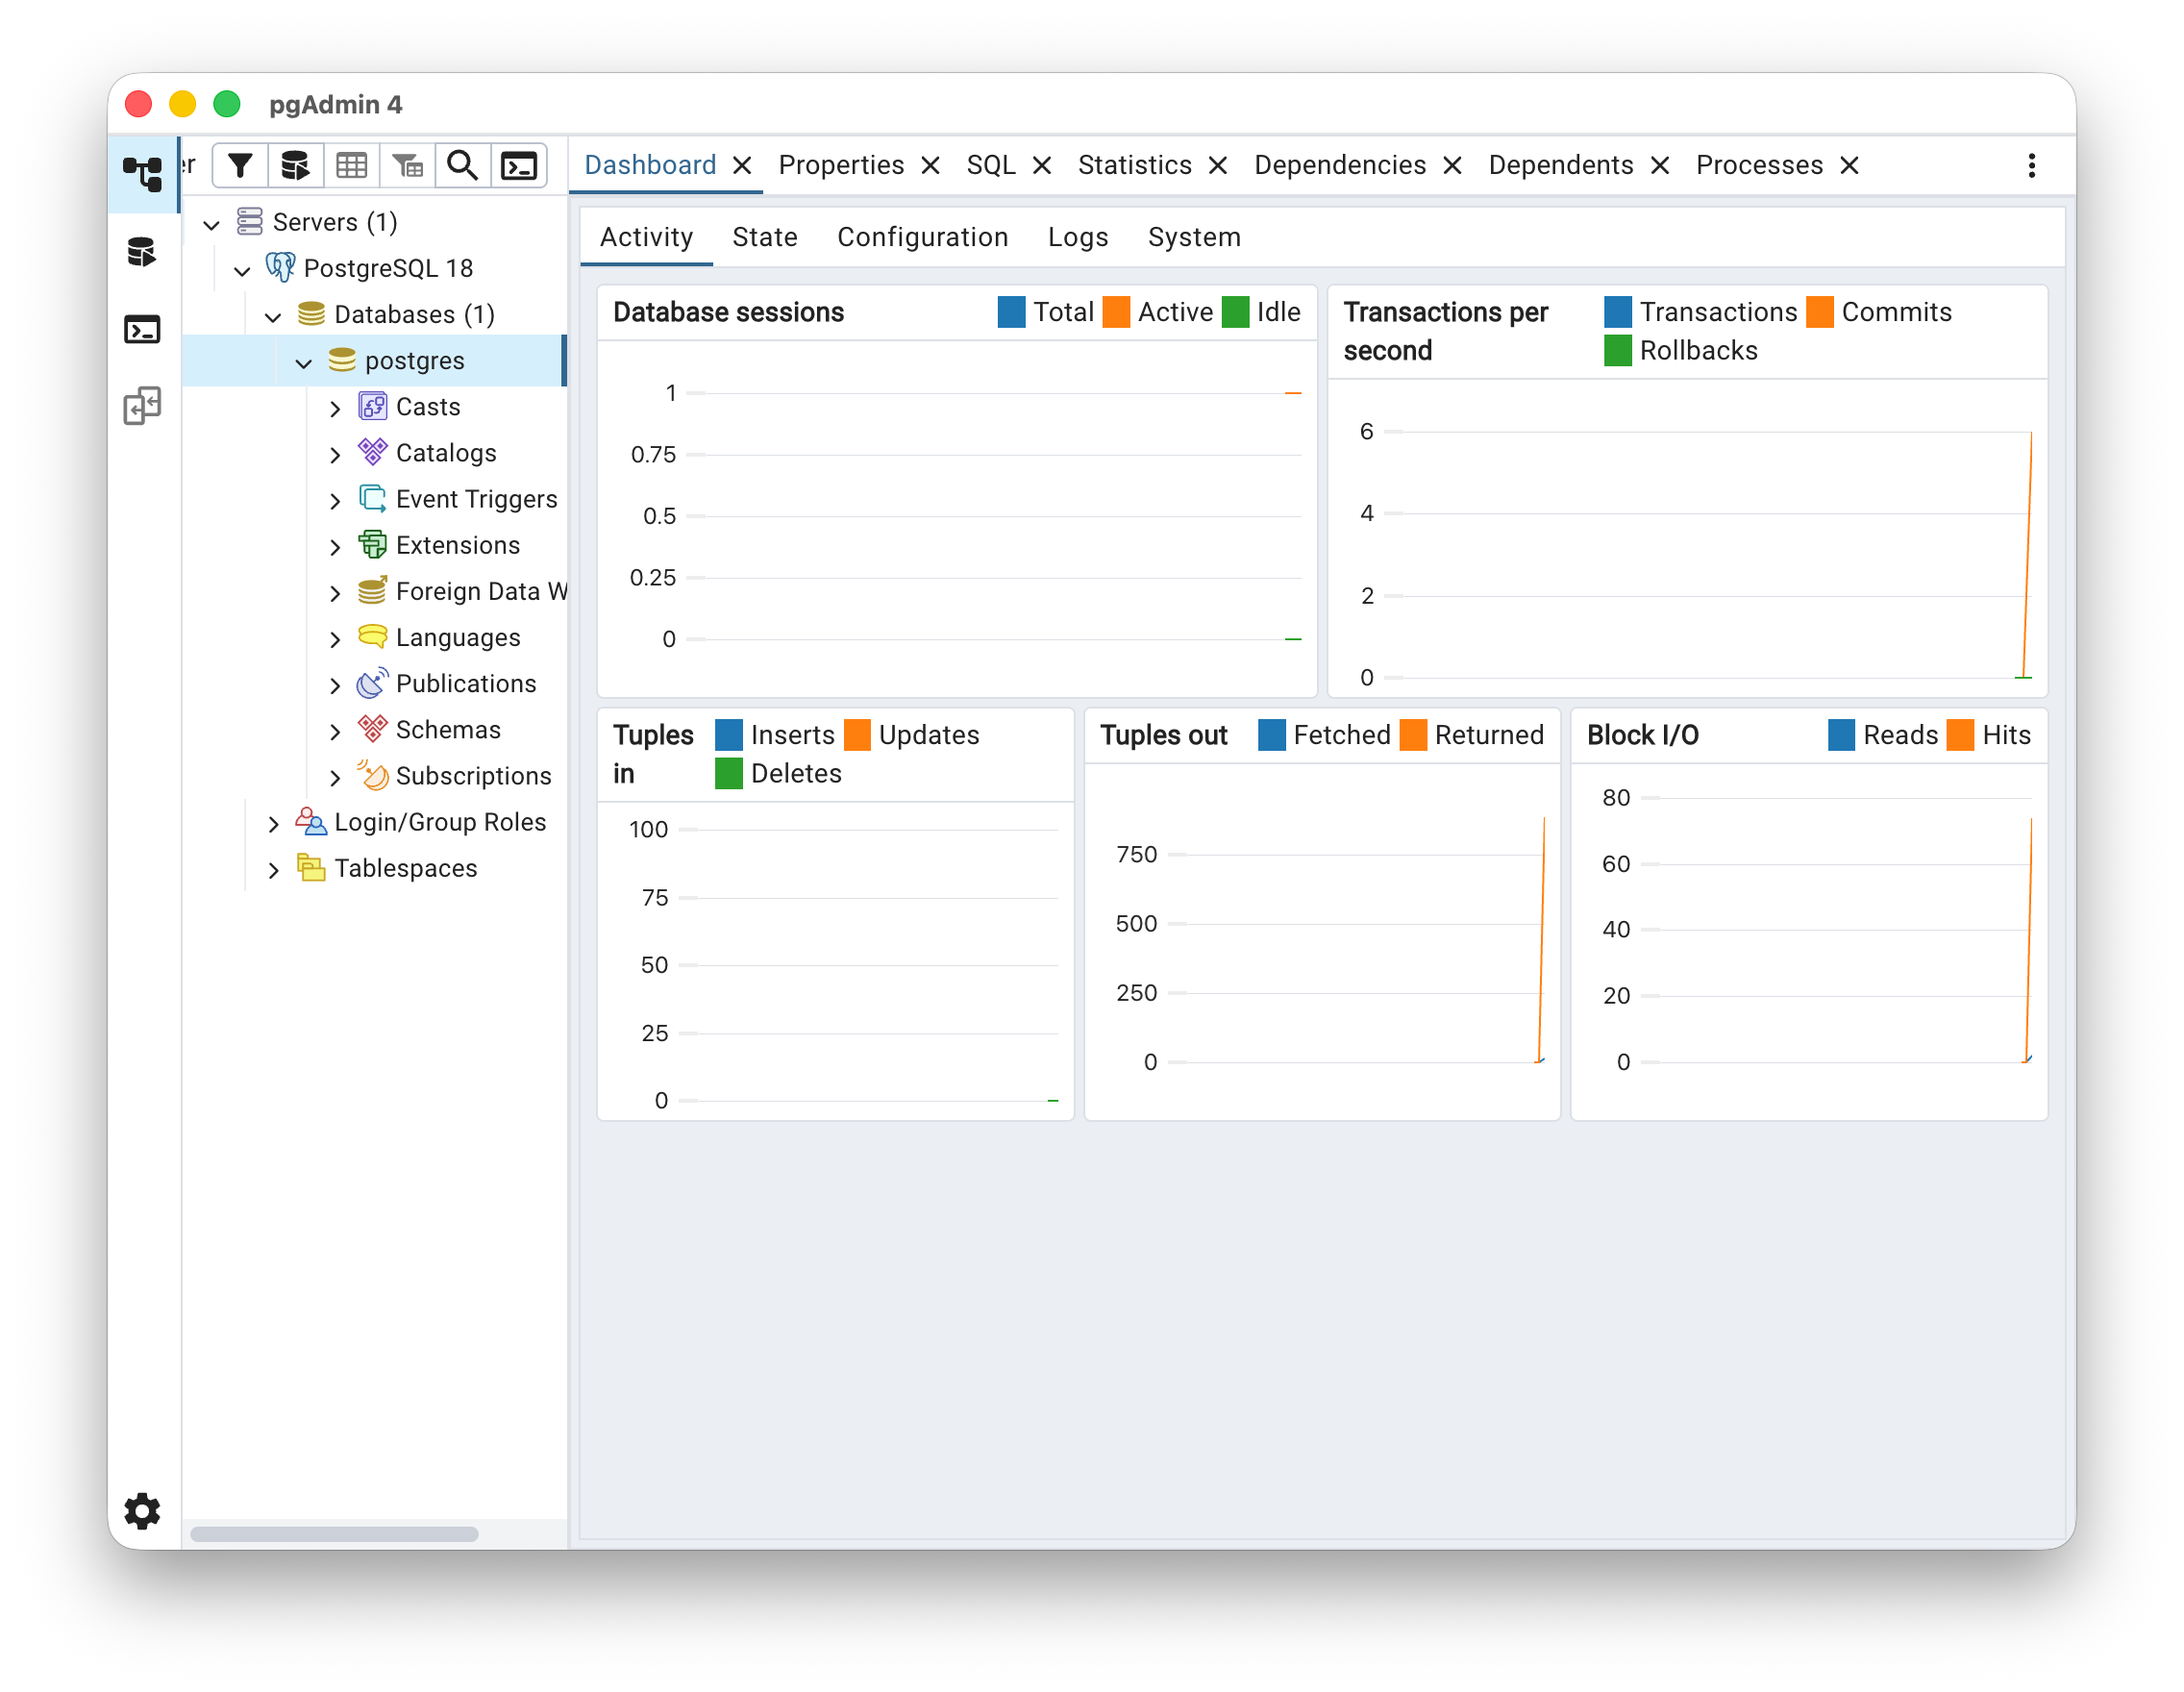
\includegraphics[width=.95\textwidth]{screen76.png}
\end{center}


\begin{resourcebox}
The \emph{Pagila} database is a demonstration database designed to illustrate database concepts. \\

\url{https://github.com/devrimgunduz/pagila} \\

To install the ''Pagila'' demo database, download the following two files and save them to your computer. 

\begin{enumerate}
\item \url{https://www.evermann.ca/busi4720/pagila-schema.sql}
\item \url{https://www.evermann.ca/busi4720/pagila-insert-data.sql}
\end{enumerate}
\end{resourcebox}

\clearpage
\item Press the Query tool button in the toolbar.

\begin{center}
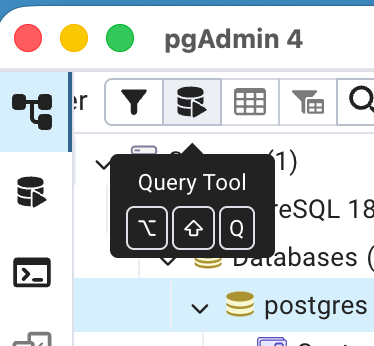
\includegraphics[width=.25\textwidth]{screen77.png}
\end{center}

\item In the Query Tool, click the ''Open File'' button.

\begin{center}
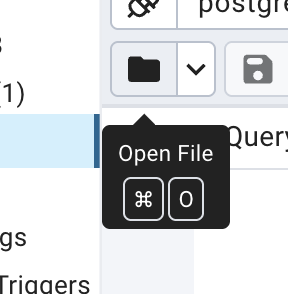
\includegraphics[width=.25\textwidth]{screen78.png}
\end{center}

\item Find and open the downloaded file ''pagila-schema.sql'' 

\begin{center}
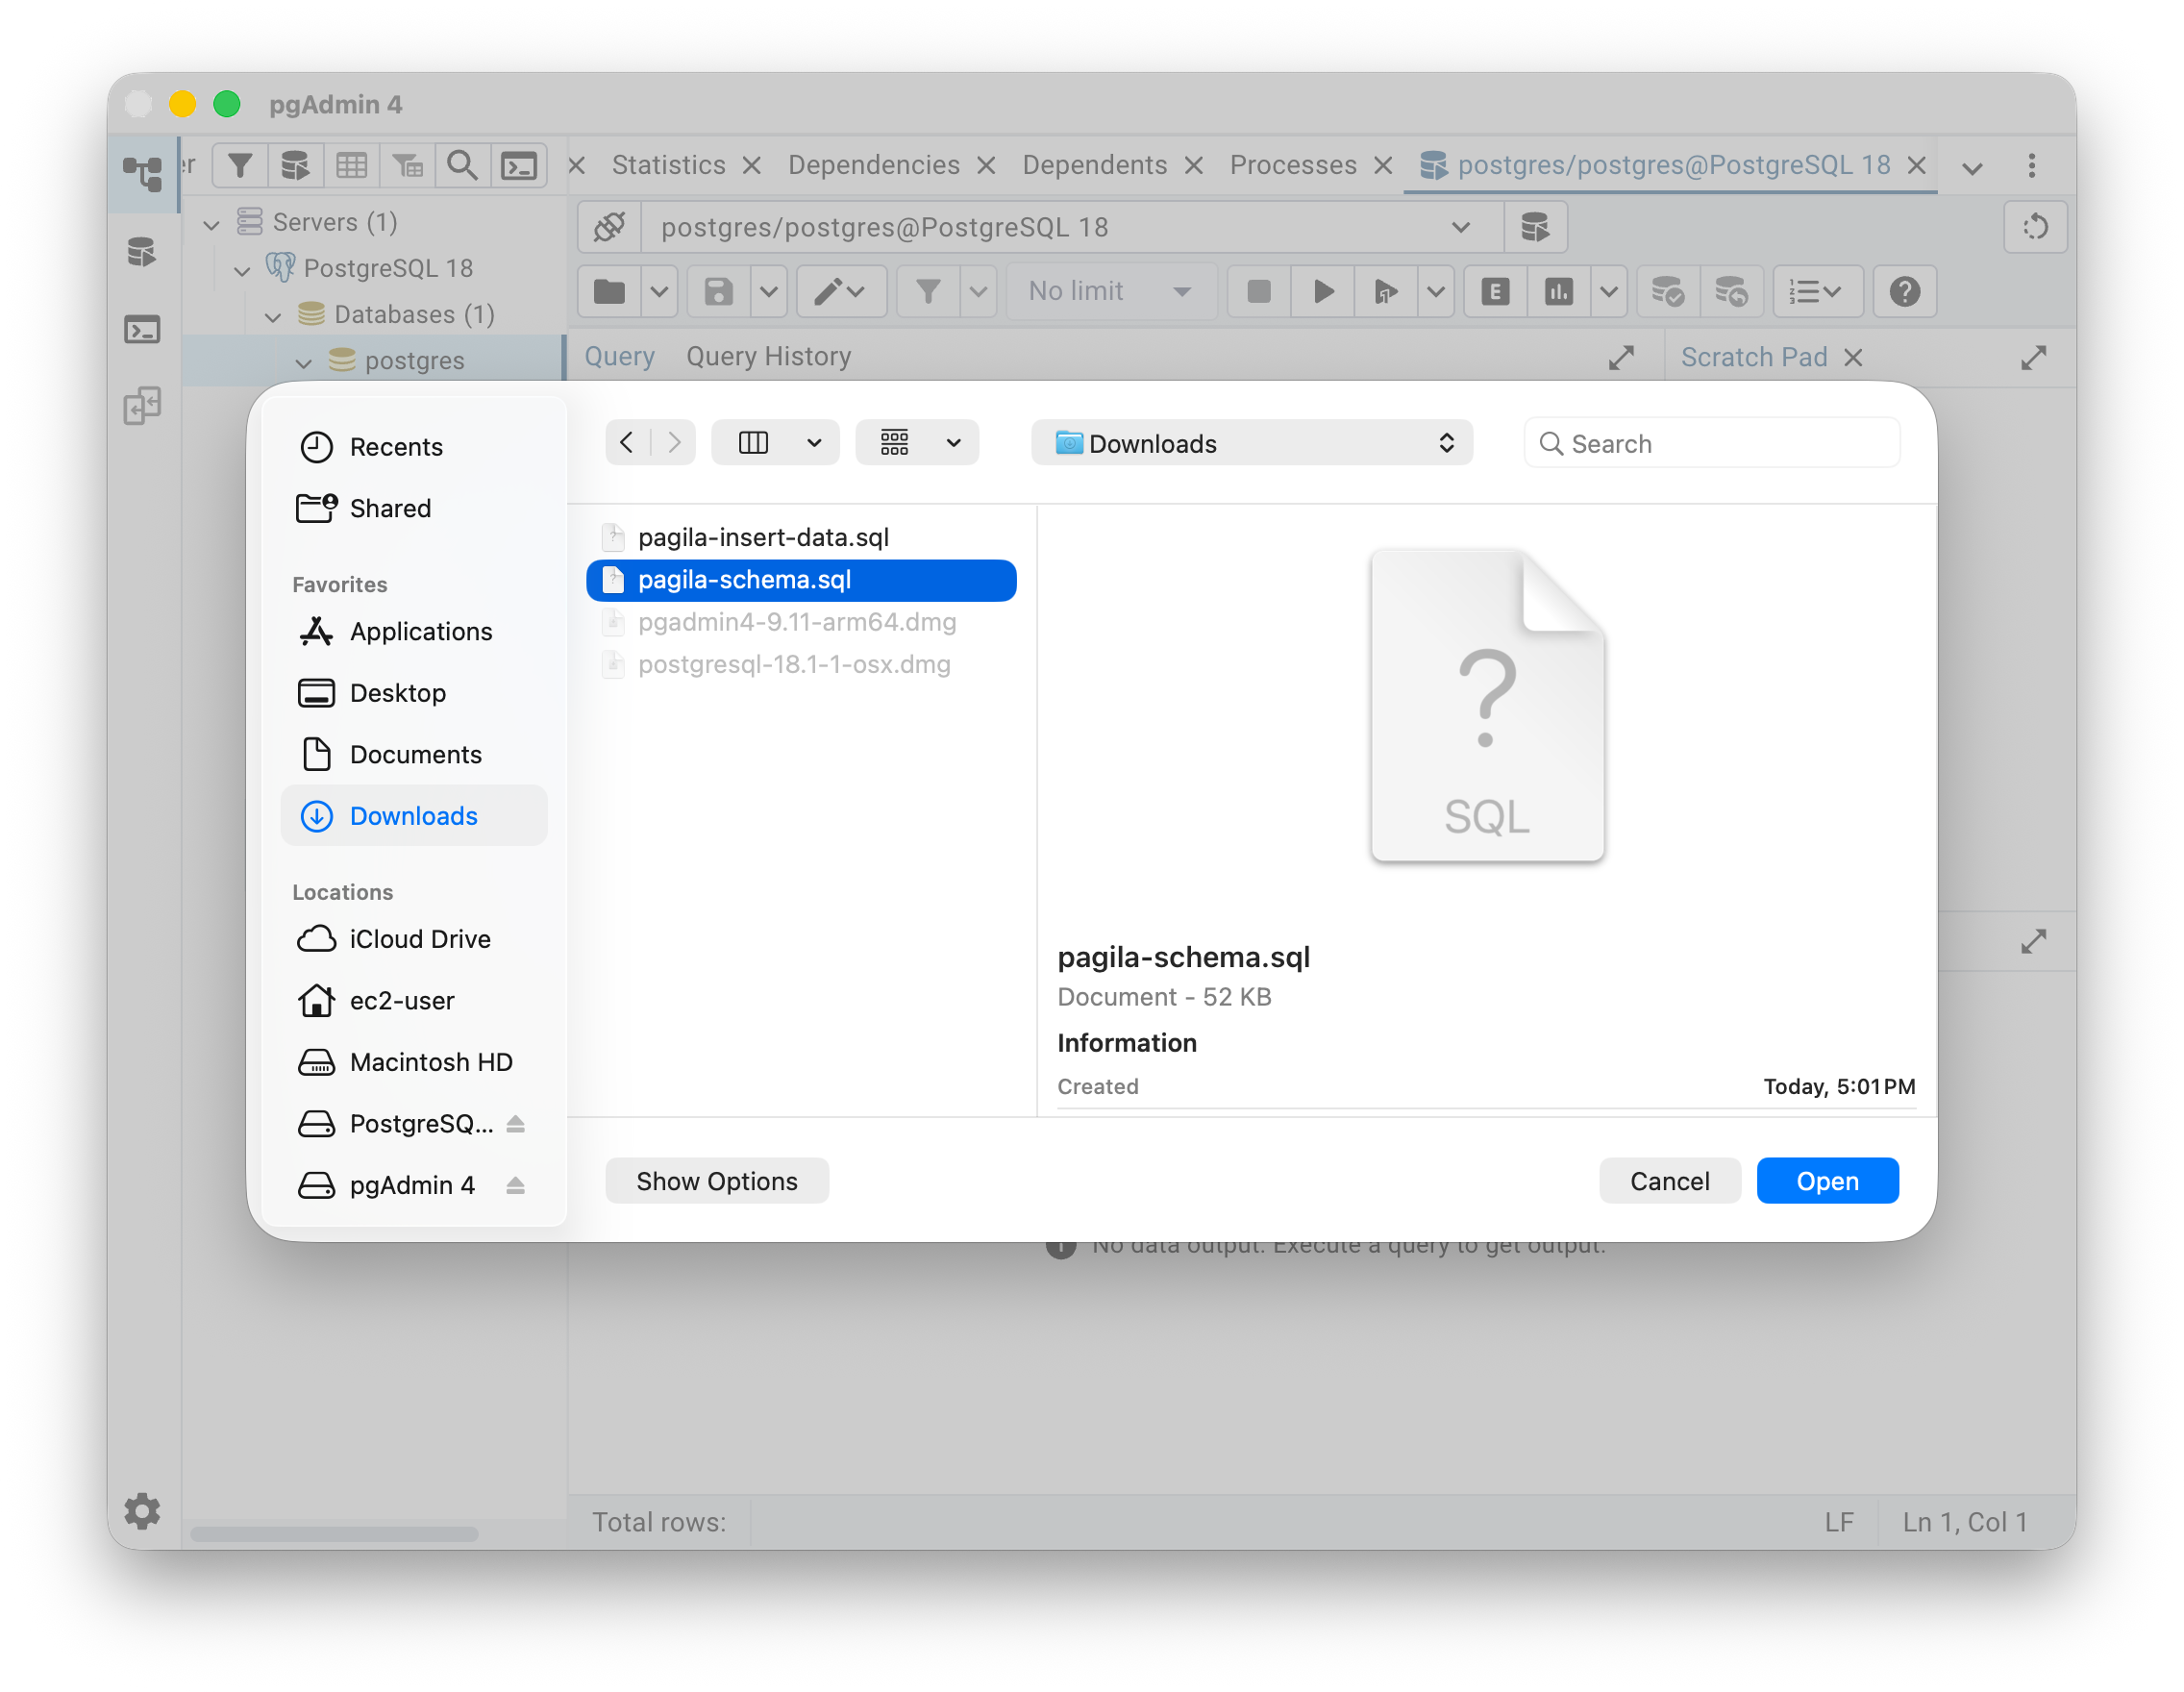
\includegraphics[width=.95\textwidth]{screen79.png}
\end{center}

\clearpage
\item In the Query Tool, click the ''Execute Script'' button.

\begin{center}
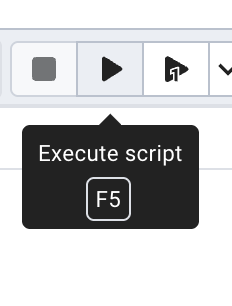
\includegraphics[width=.25\textwidth]{screen80.png}
\end{center}

\item In the pgAdmin application, choose ''Query Tool'' from the main again. Repeat the above three steps for the file ''pagila-insert-data.sql''

You have now installed the Pagila database.

\end{itemize}

\clearpage
\subsection{Installing Neo4J}

\begin{resourcebox}
Neo4J is a graph database that is available for Windows and MacOS systems. There are different ways to install it but the easiest is to use the Neo4J for Desktop version that is intended for database developers. The installation application for this Neo4J version can be found via its website. \\

\url{https://www.neo4j.com/download/}
\end{resourcebox}

\begin{itemize}

\item Navigate to the Neo4J for Desktop download page and click the ''Download'' button.

\begin{center}
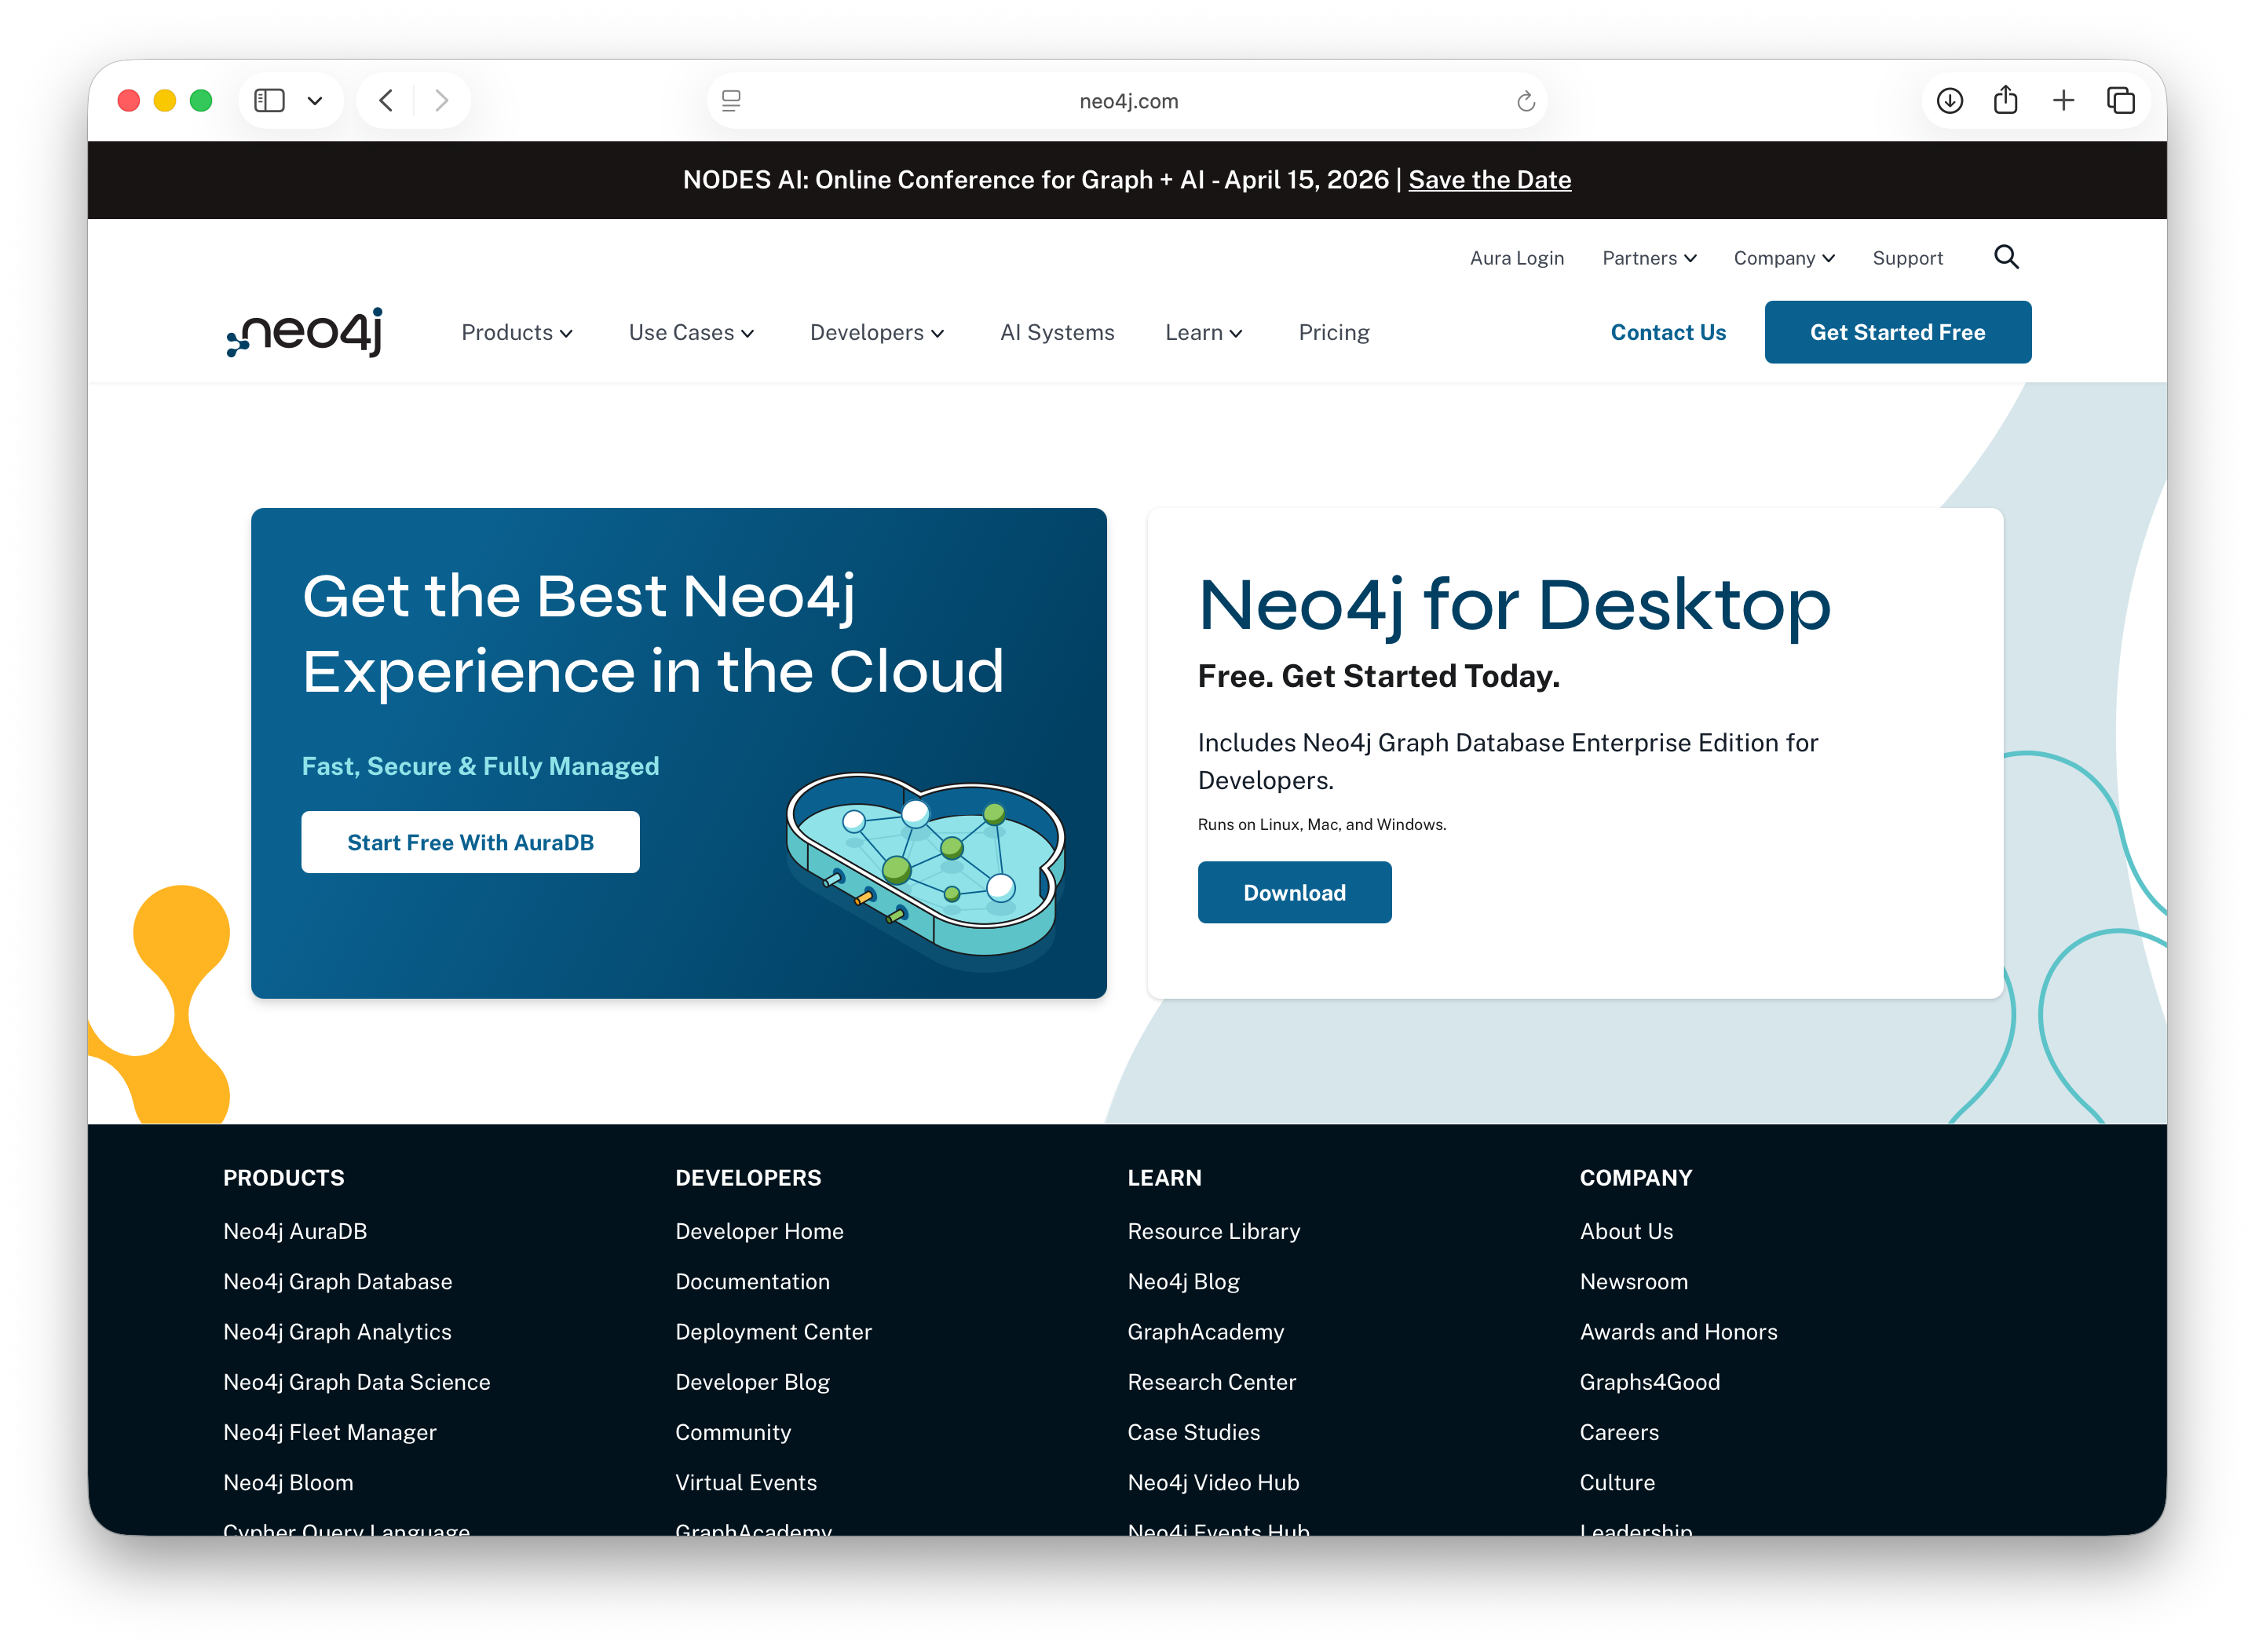
\includegraphics[width=.95\textwidth]{screen81.png}
\end{center}

\clearpage
\item After the download, double-click on the downloaded file to open it. You will a window with Neo4J Desktop and the Applications folder. In this window, drag and drop the Neo4J icon to the Applications icon.

\begin{center}
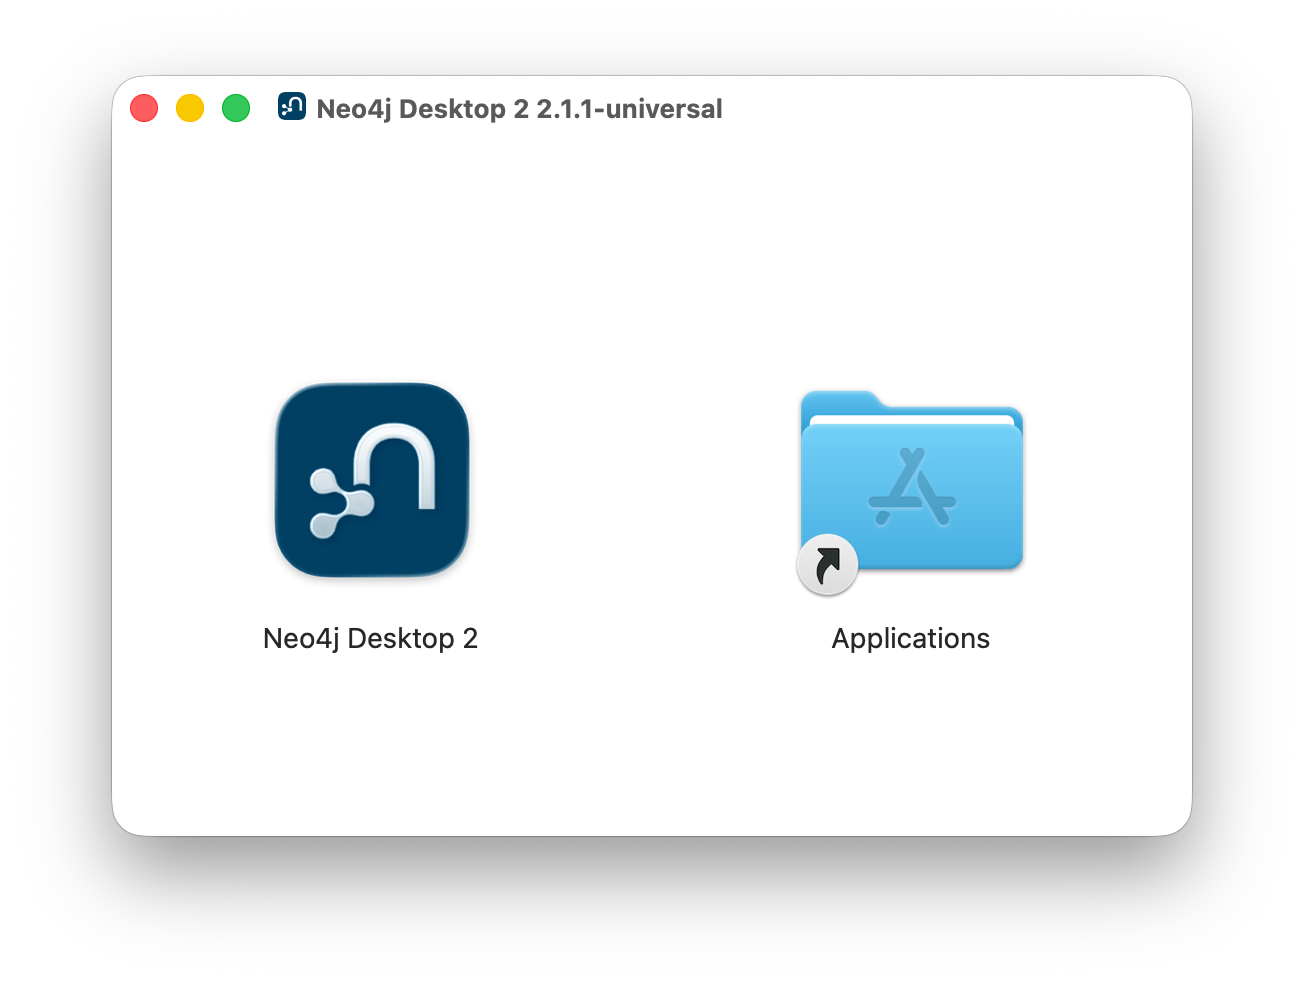
\includegraphics[width=.65\textwidth]{screen82.png}
\end{center}

\item Using the Finder application, navigate to the Applications folder and find the Neo4J application. Double-click to launch it.

\begin{center}
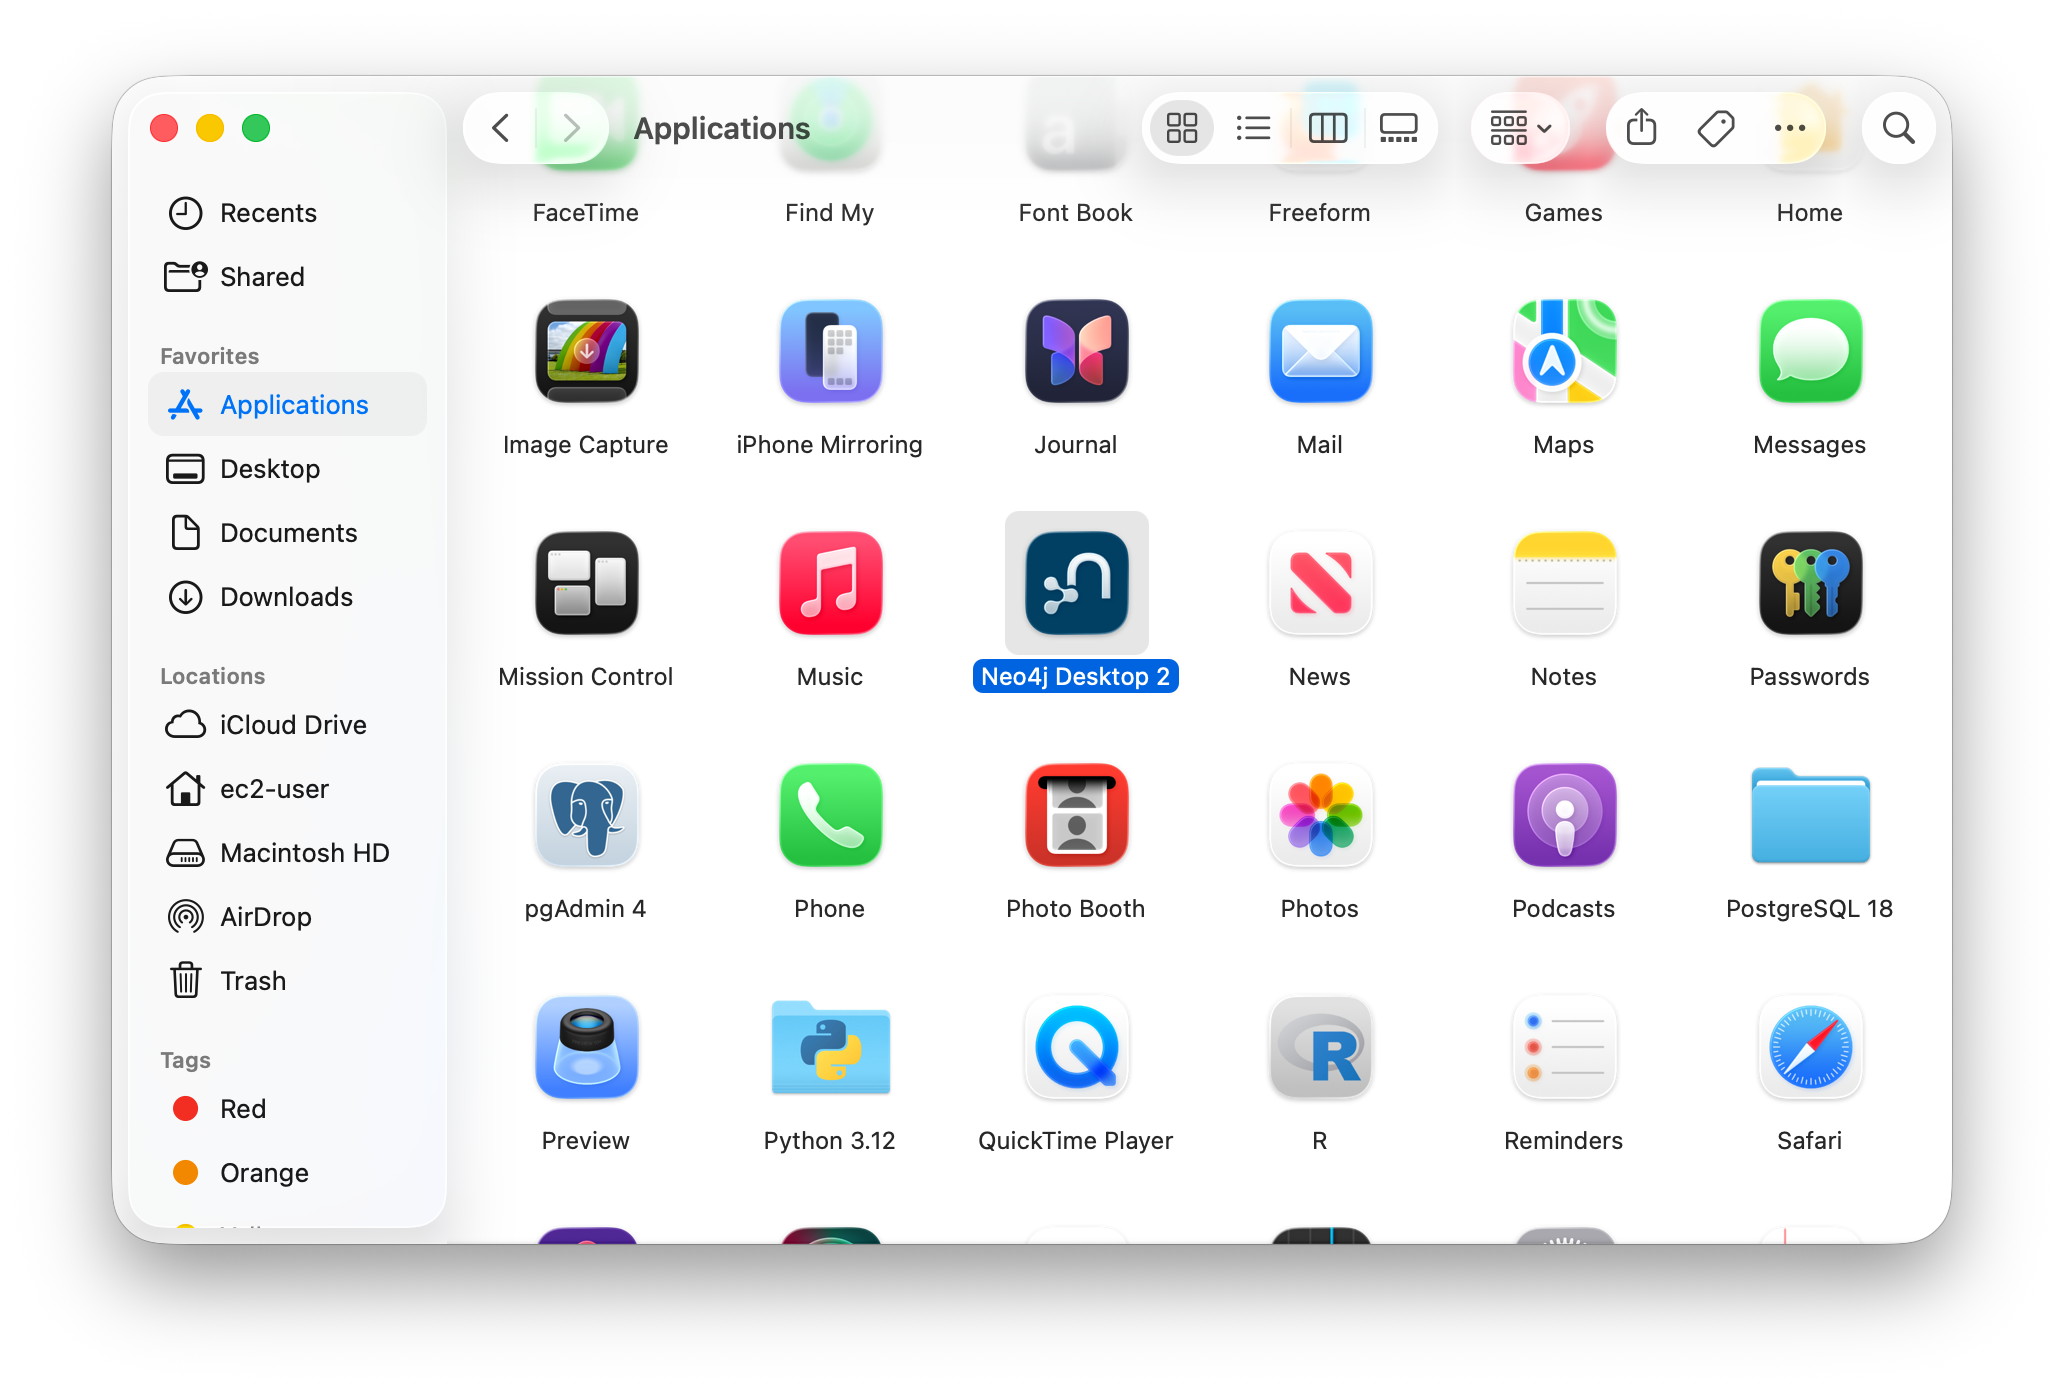
\includegraphics[width=.95\textwidth]{screen83.png}
\end{center}

\clearpage
\item The Neo4J application will start and present you with a license agreement which you must accept by clicking the ''Continue'' button.

\begin{center}
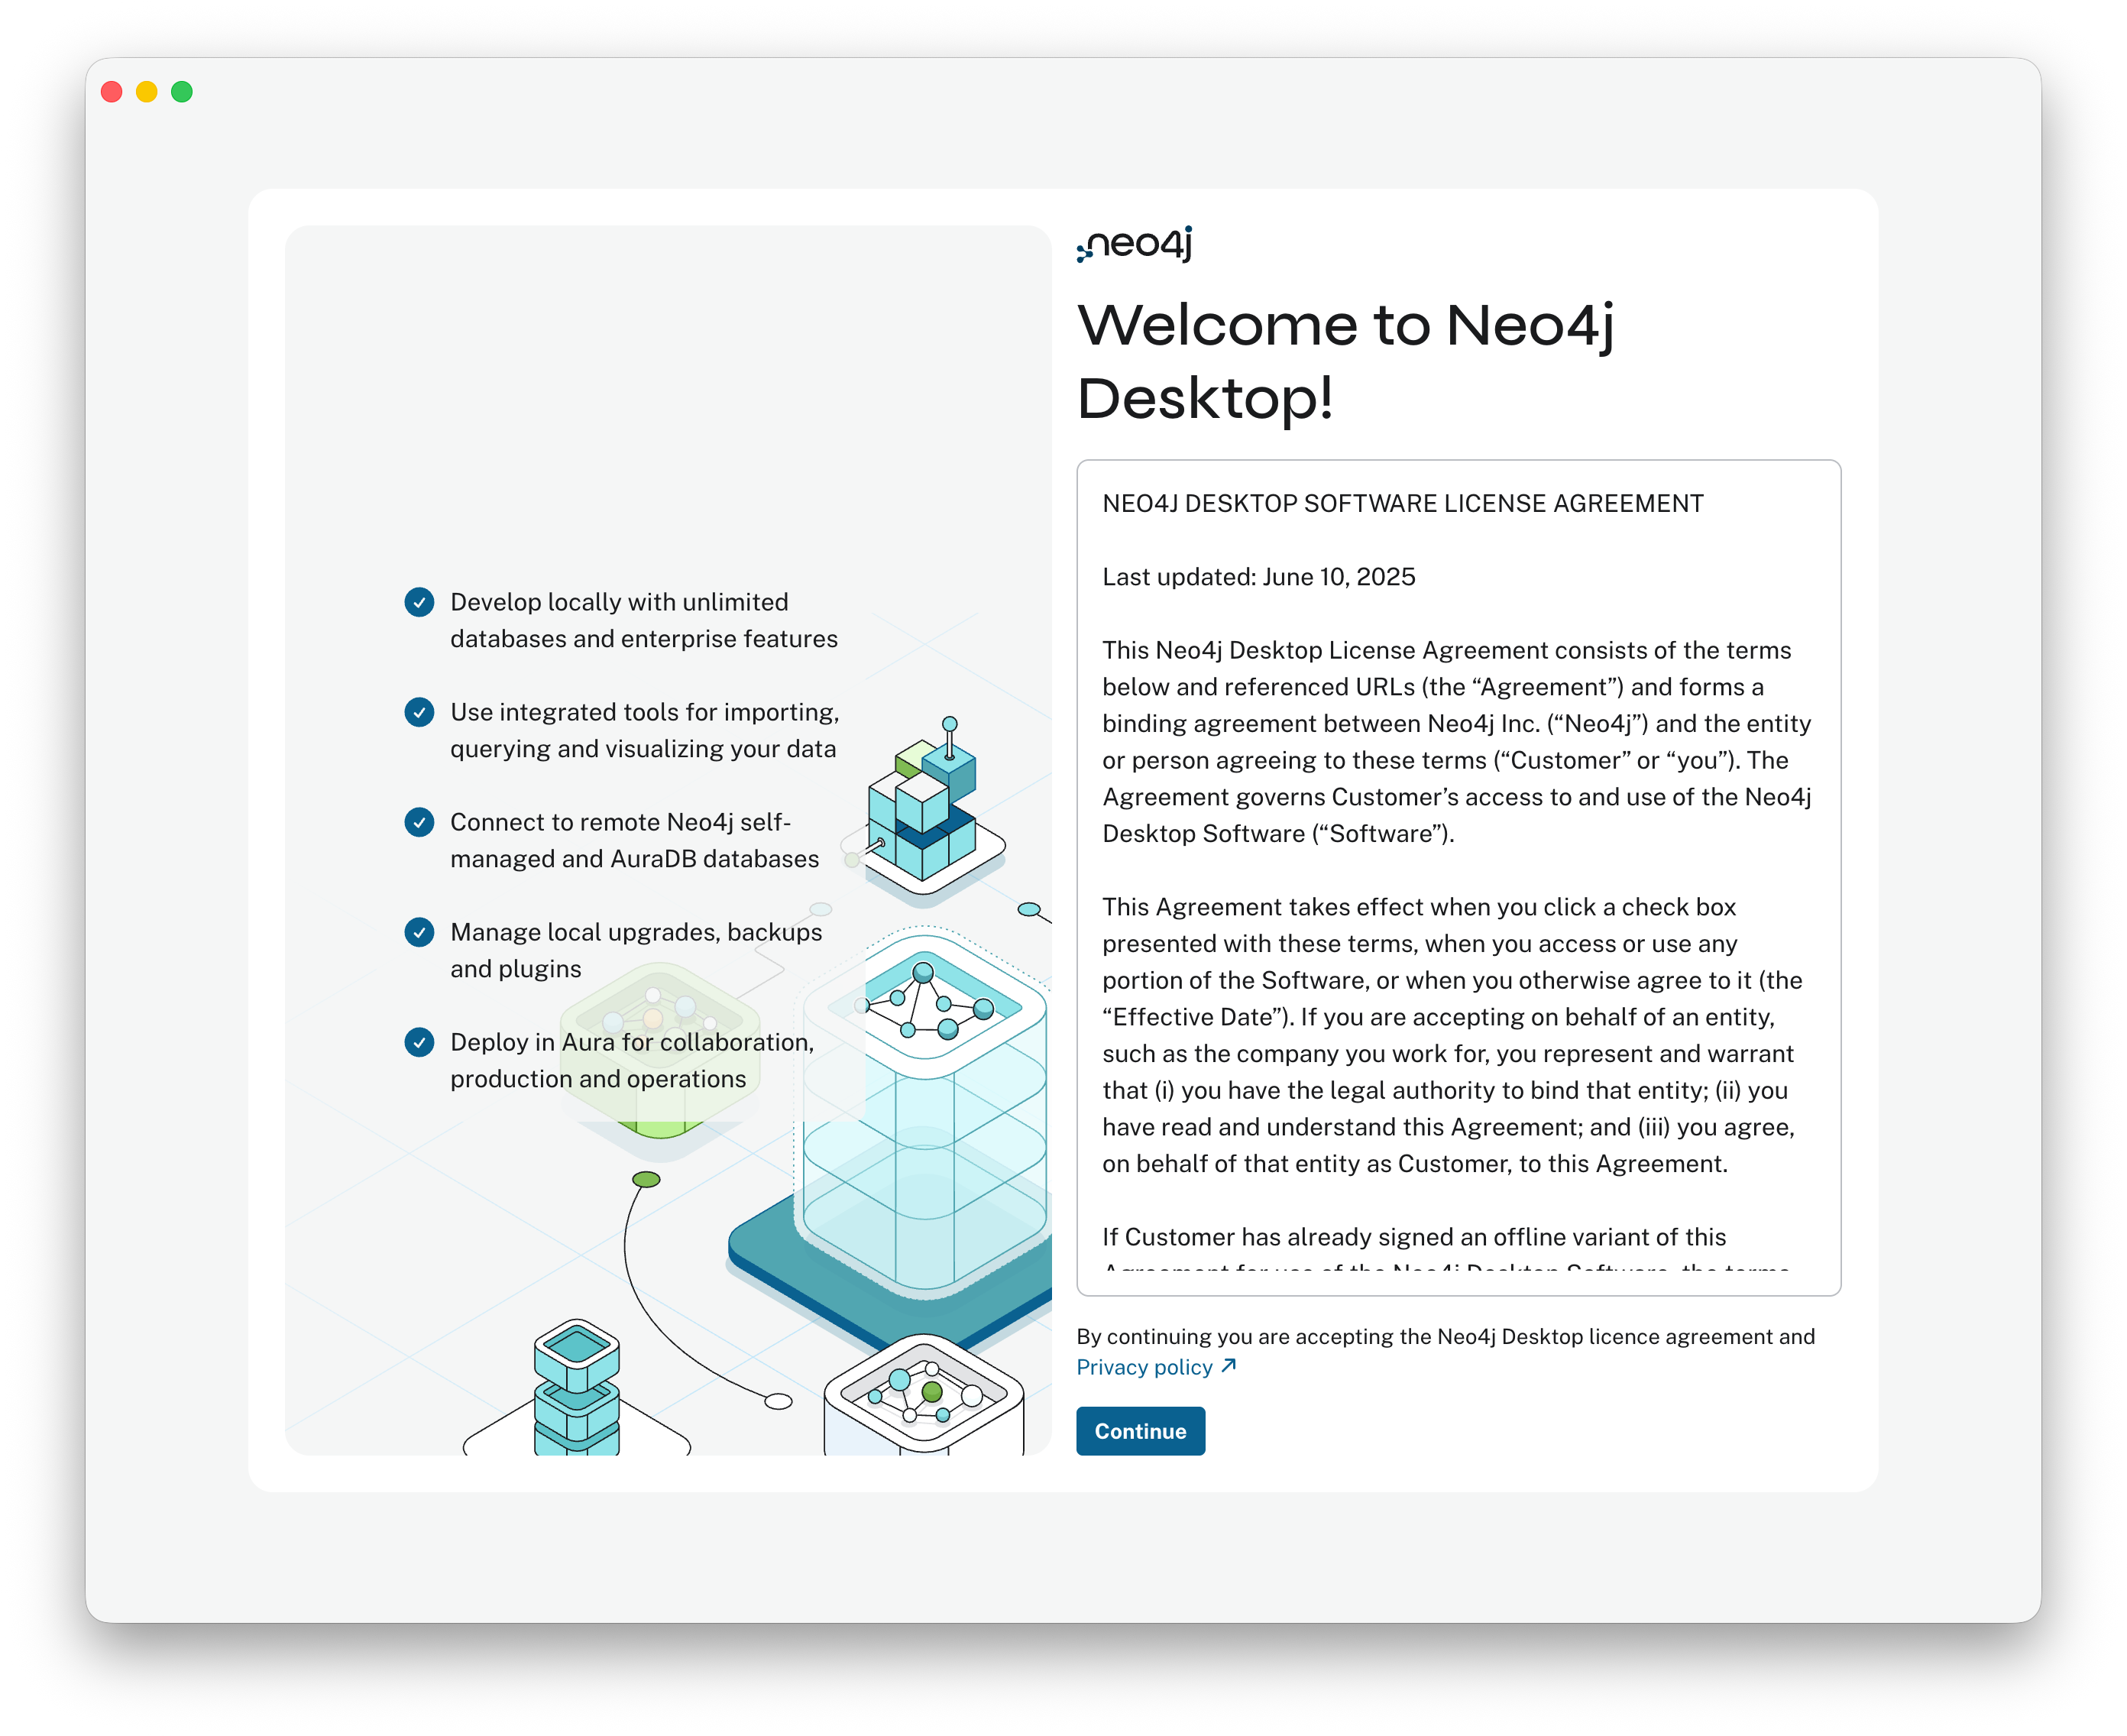
\includegraphics[width=.85\textwidth]{screen84.png}
\end{center}

\item Neo4J will ask you create a database server instance and a database in that. Click the ''Create instance'' button.

\begin{center}
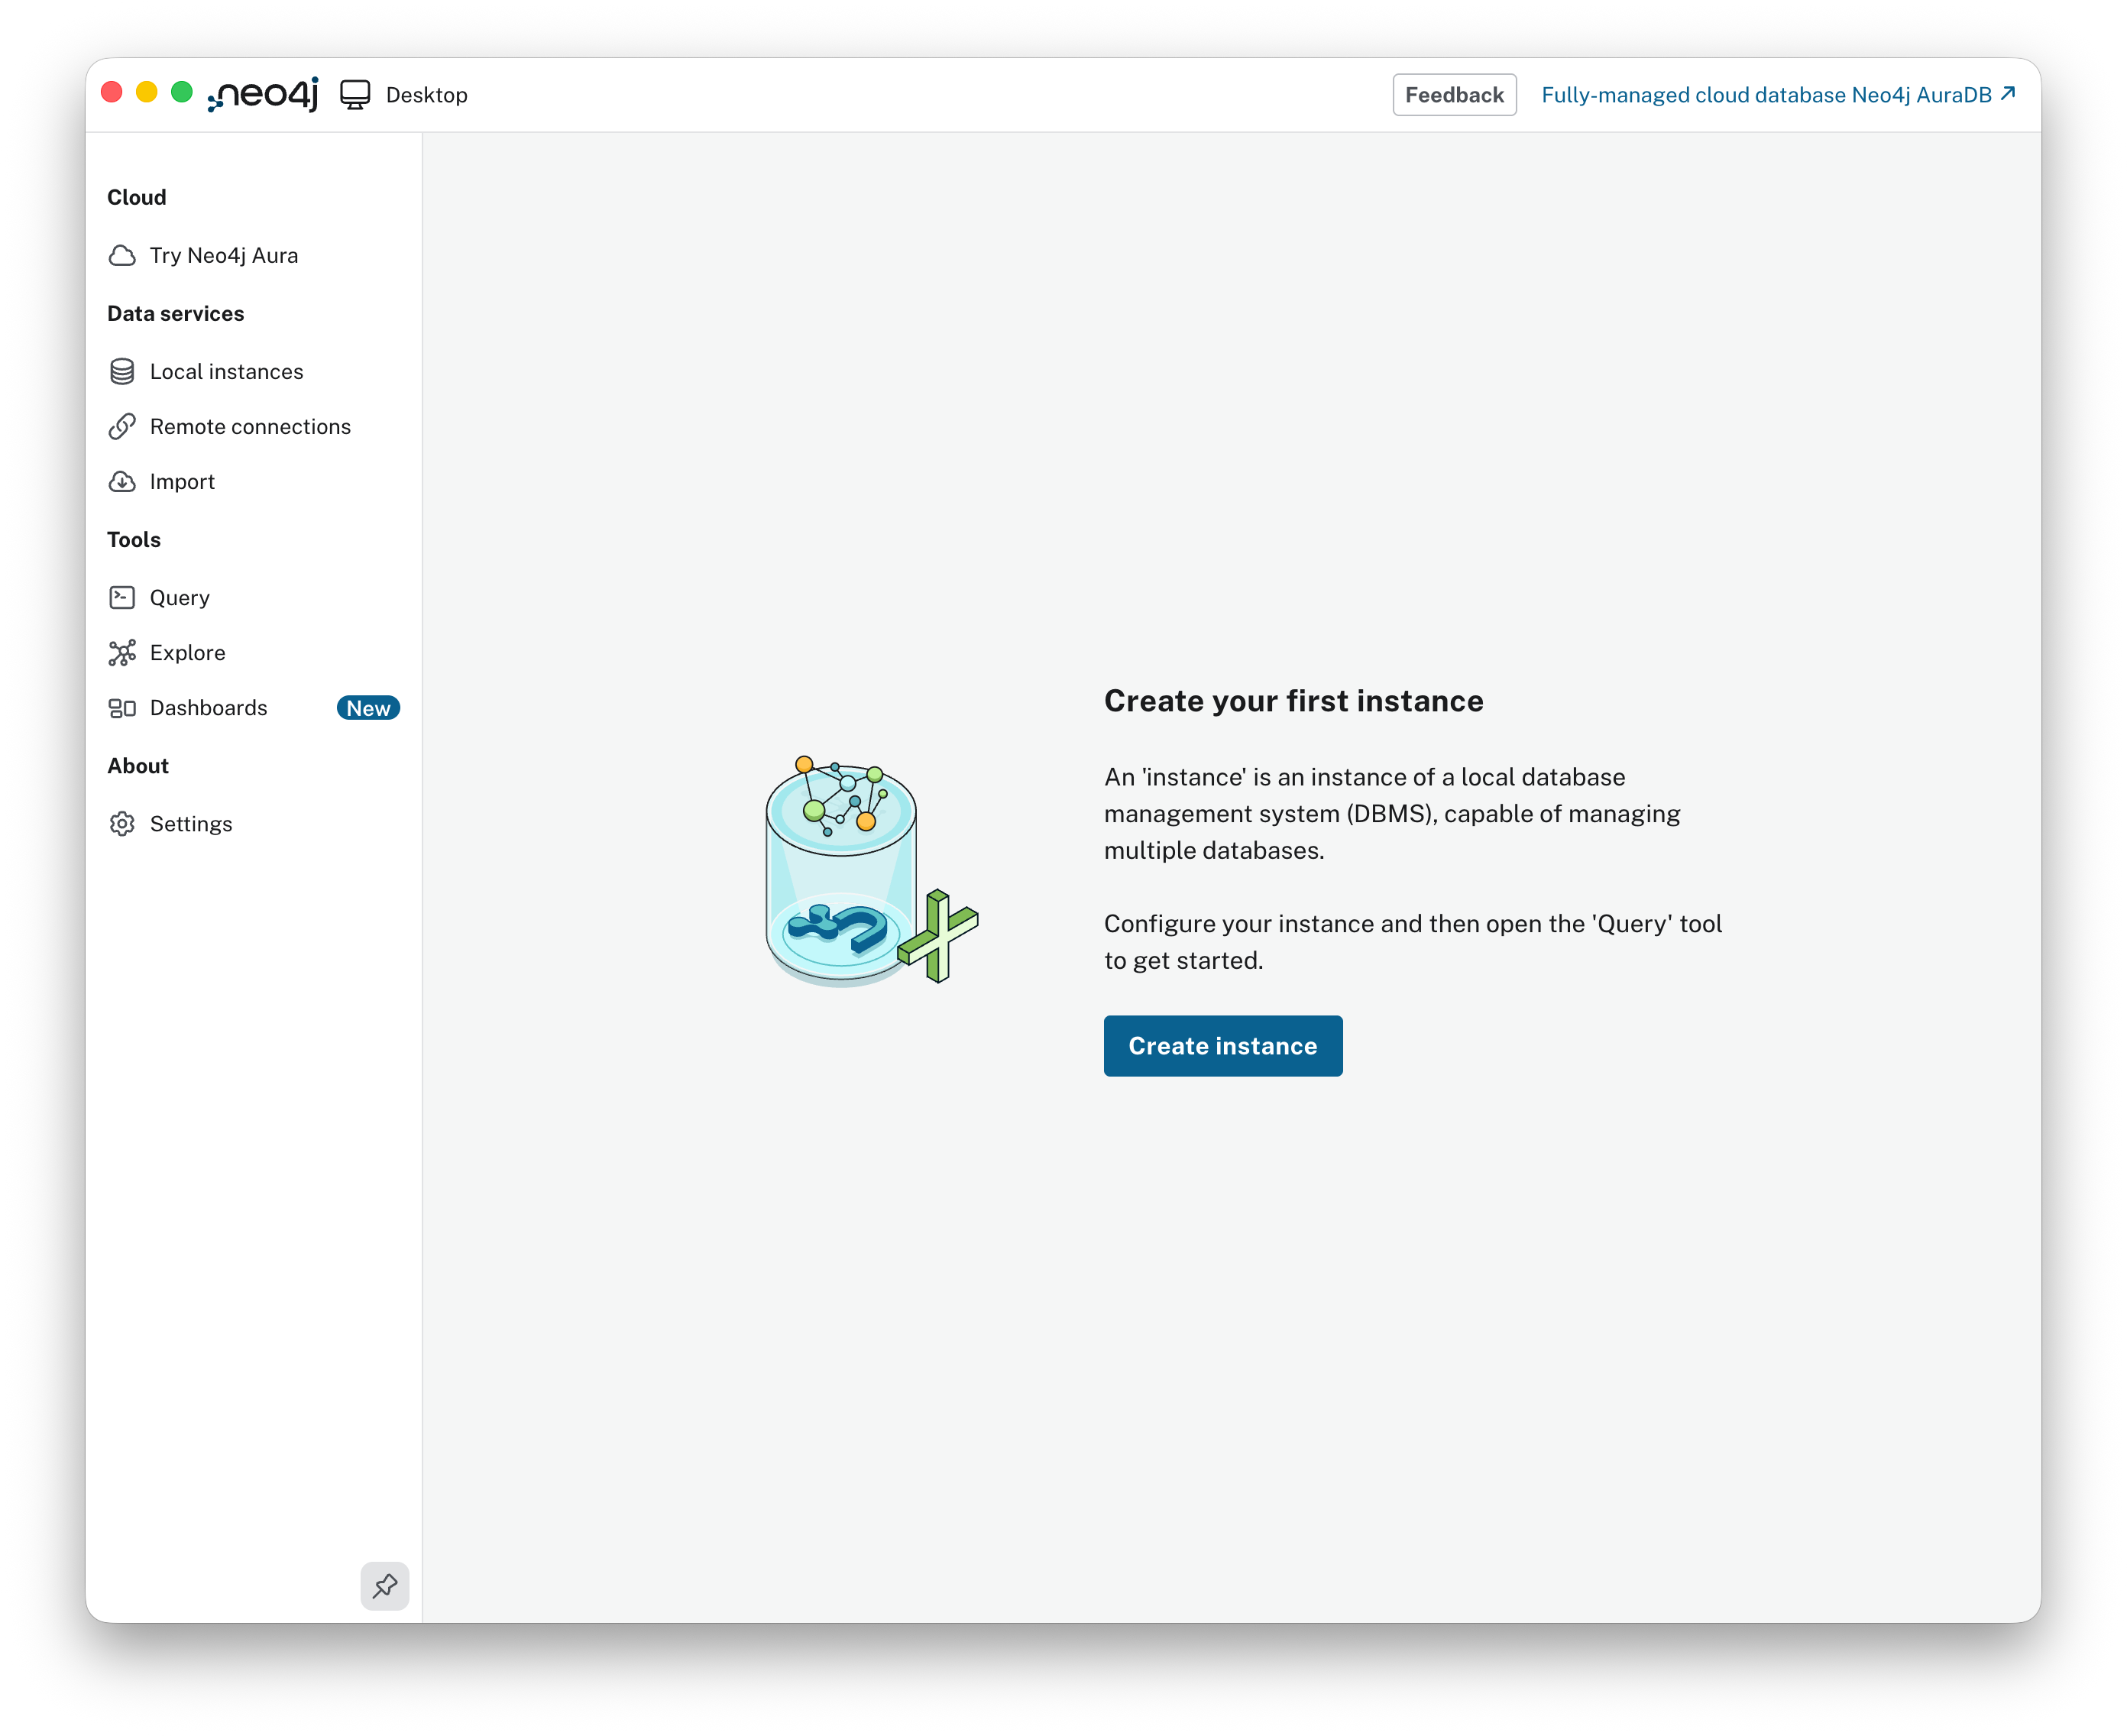
\includegraphics[width=.85\textwidth]{screen85.png}
\end{center}

\item Give the instance a name of your choice, e.g. ''busi4720'' and provide a new password for the database user. Select the option to load from .dump, .backup or .tar file.

\begin{center}
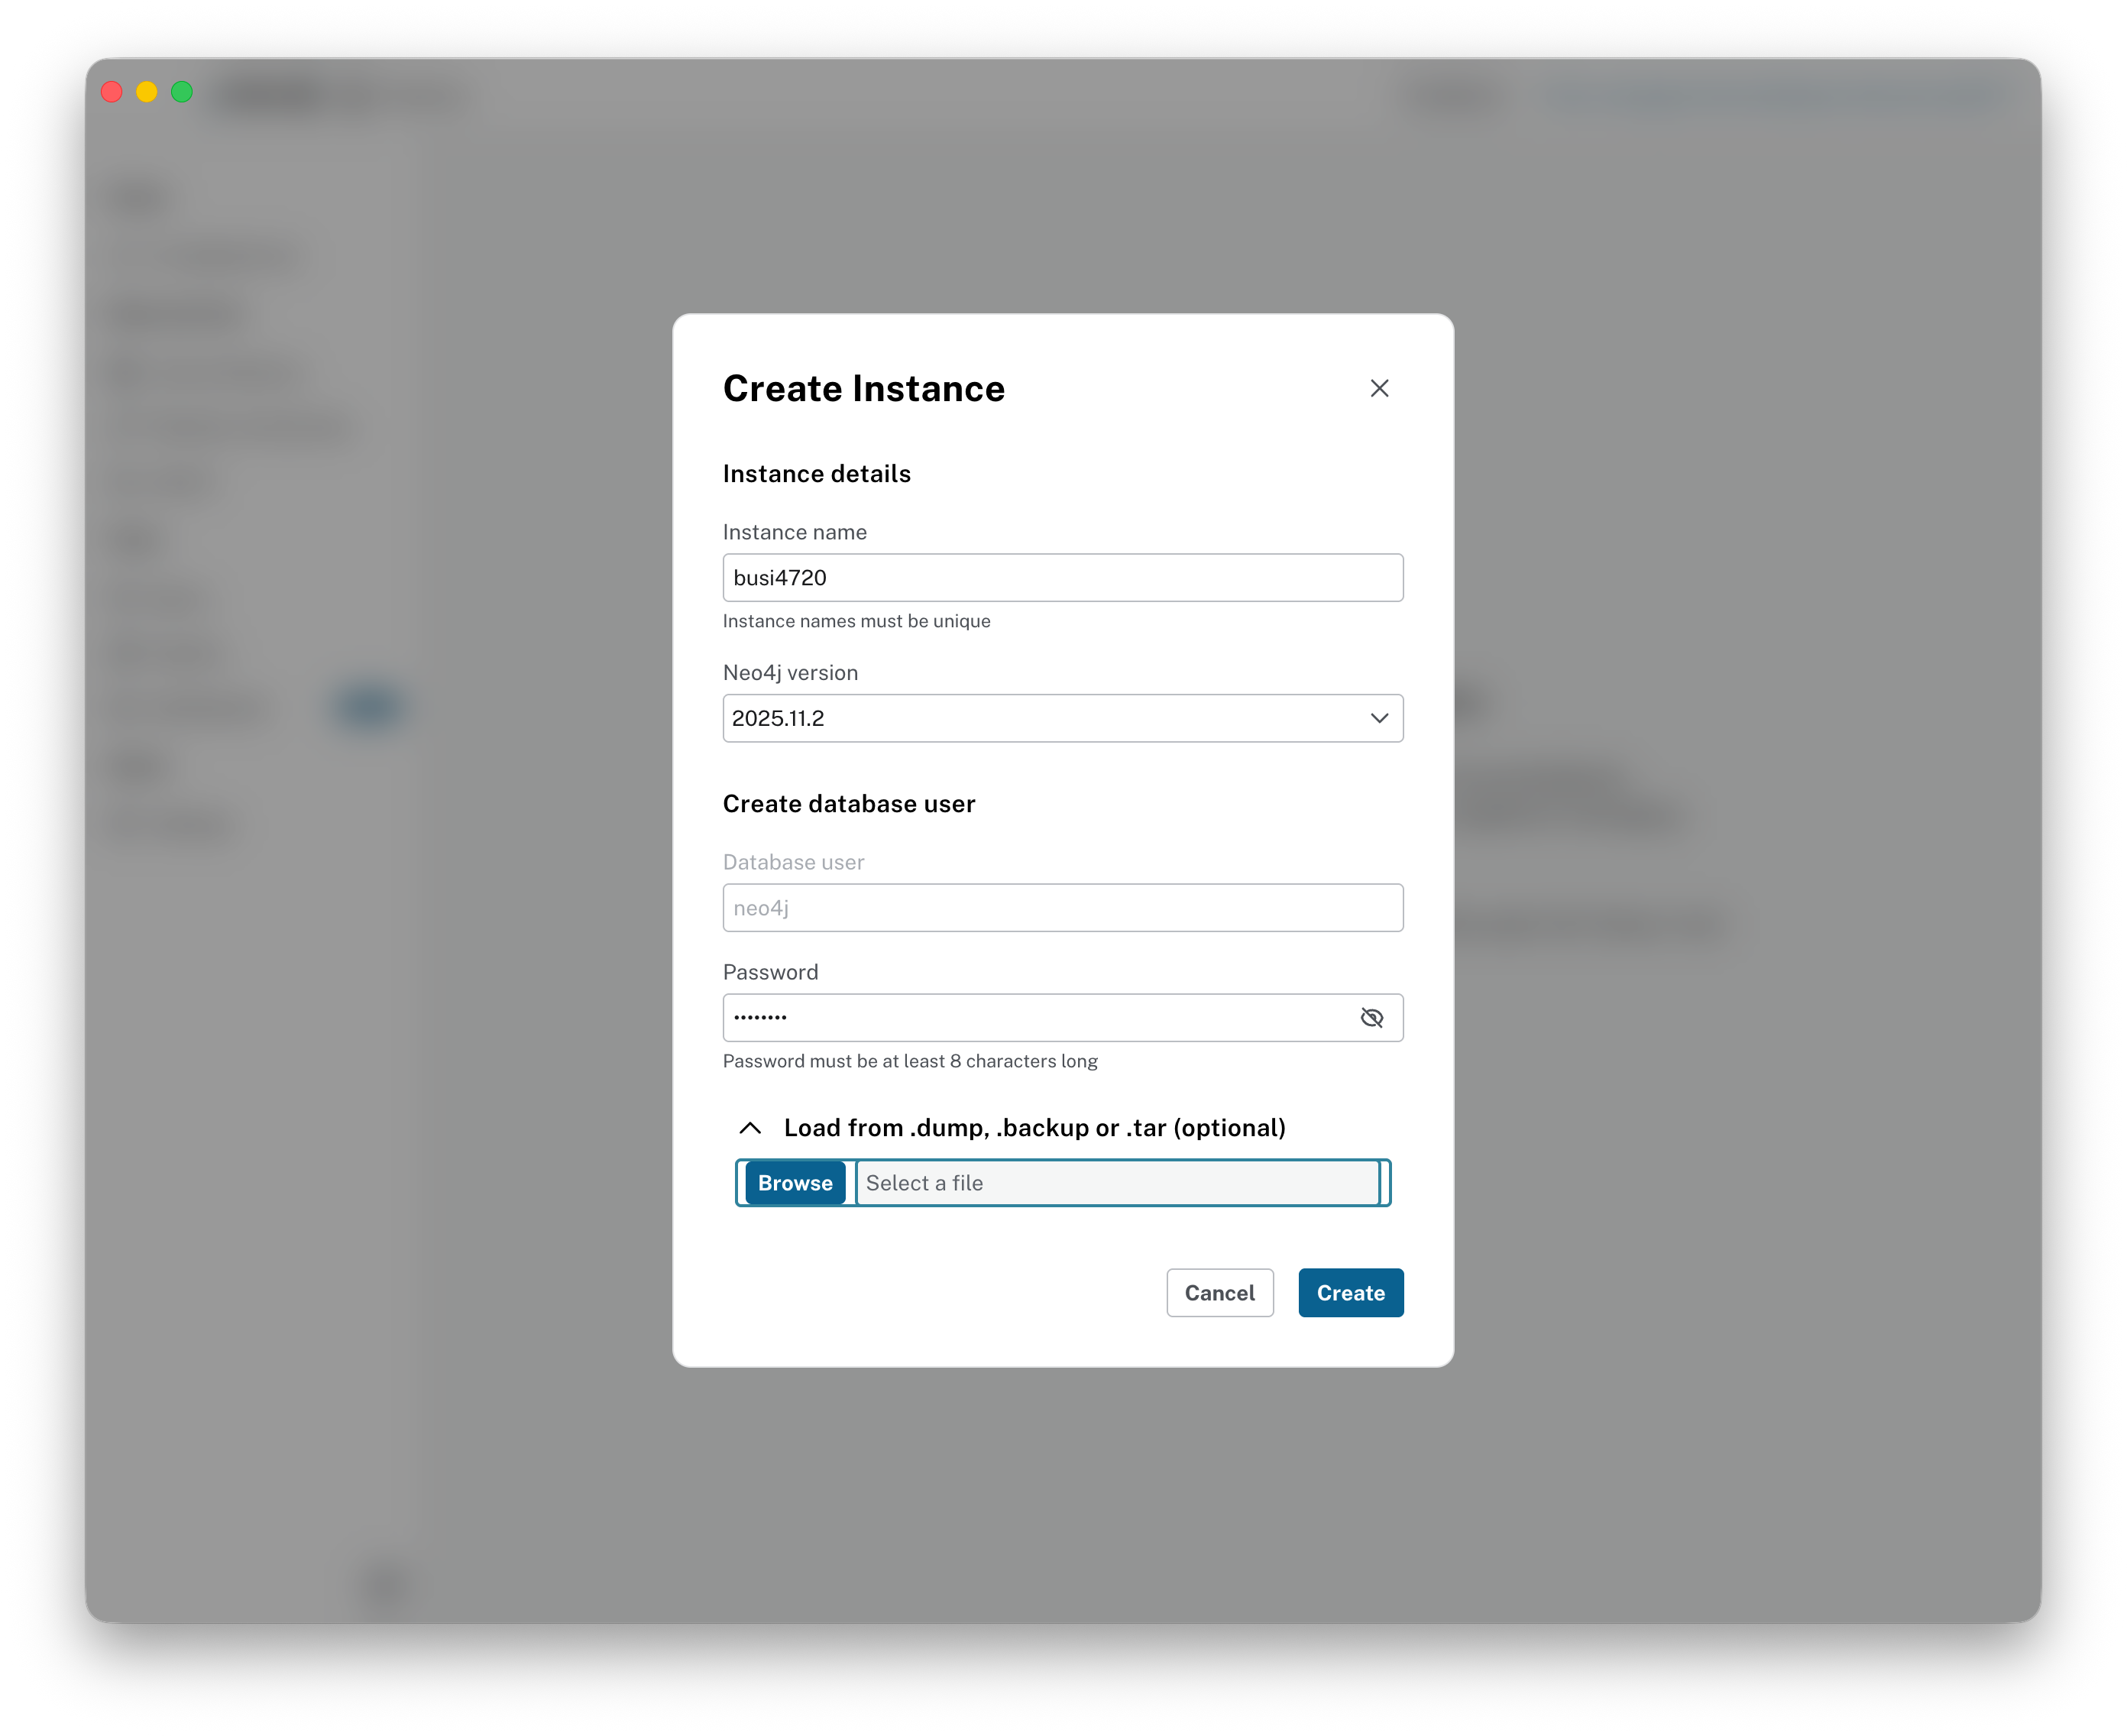
\includegraphics[width=.85\textwidth]{screen86.png}
\end{center}

\begin{resourcebox}
The \emph{Pagila} database is a demonstration database designed to illustrate database concepts. A version of Pagila for Neo4J is available for download. \\

Download and save the following file to your computer.

\begin{enumerate}
\item \url{https://www.evermann.ca/busi4720/neo4j_db_pagila.dump}
\end{enumerate}
\end{resourcebox}

\clearpage
\item In the Neo4J application, select the ''Browse'' button and find and open the file you just downloaded.

\begin{center}
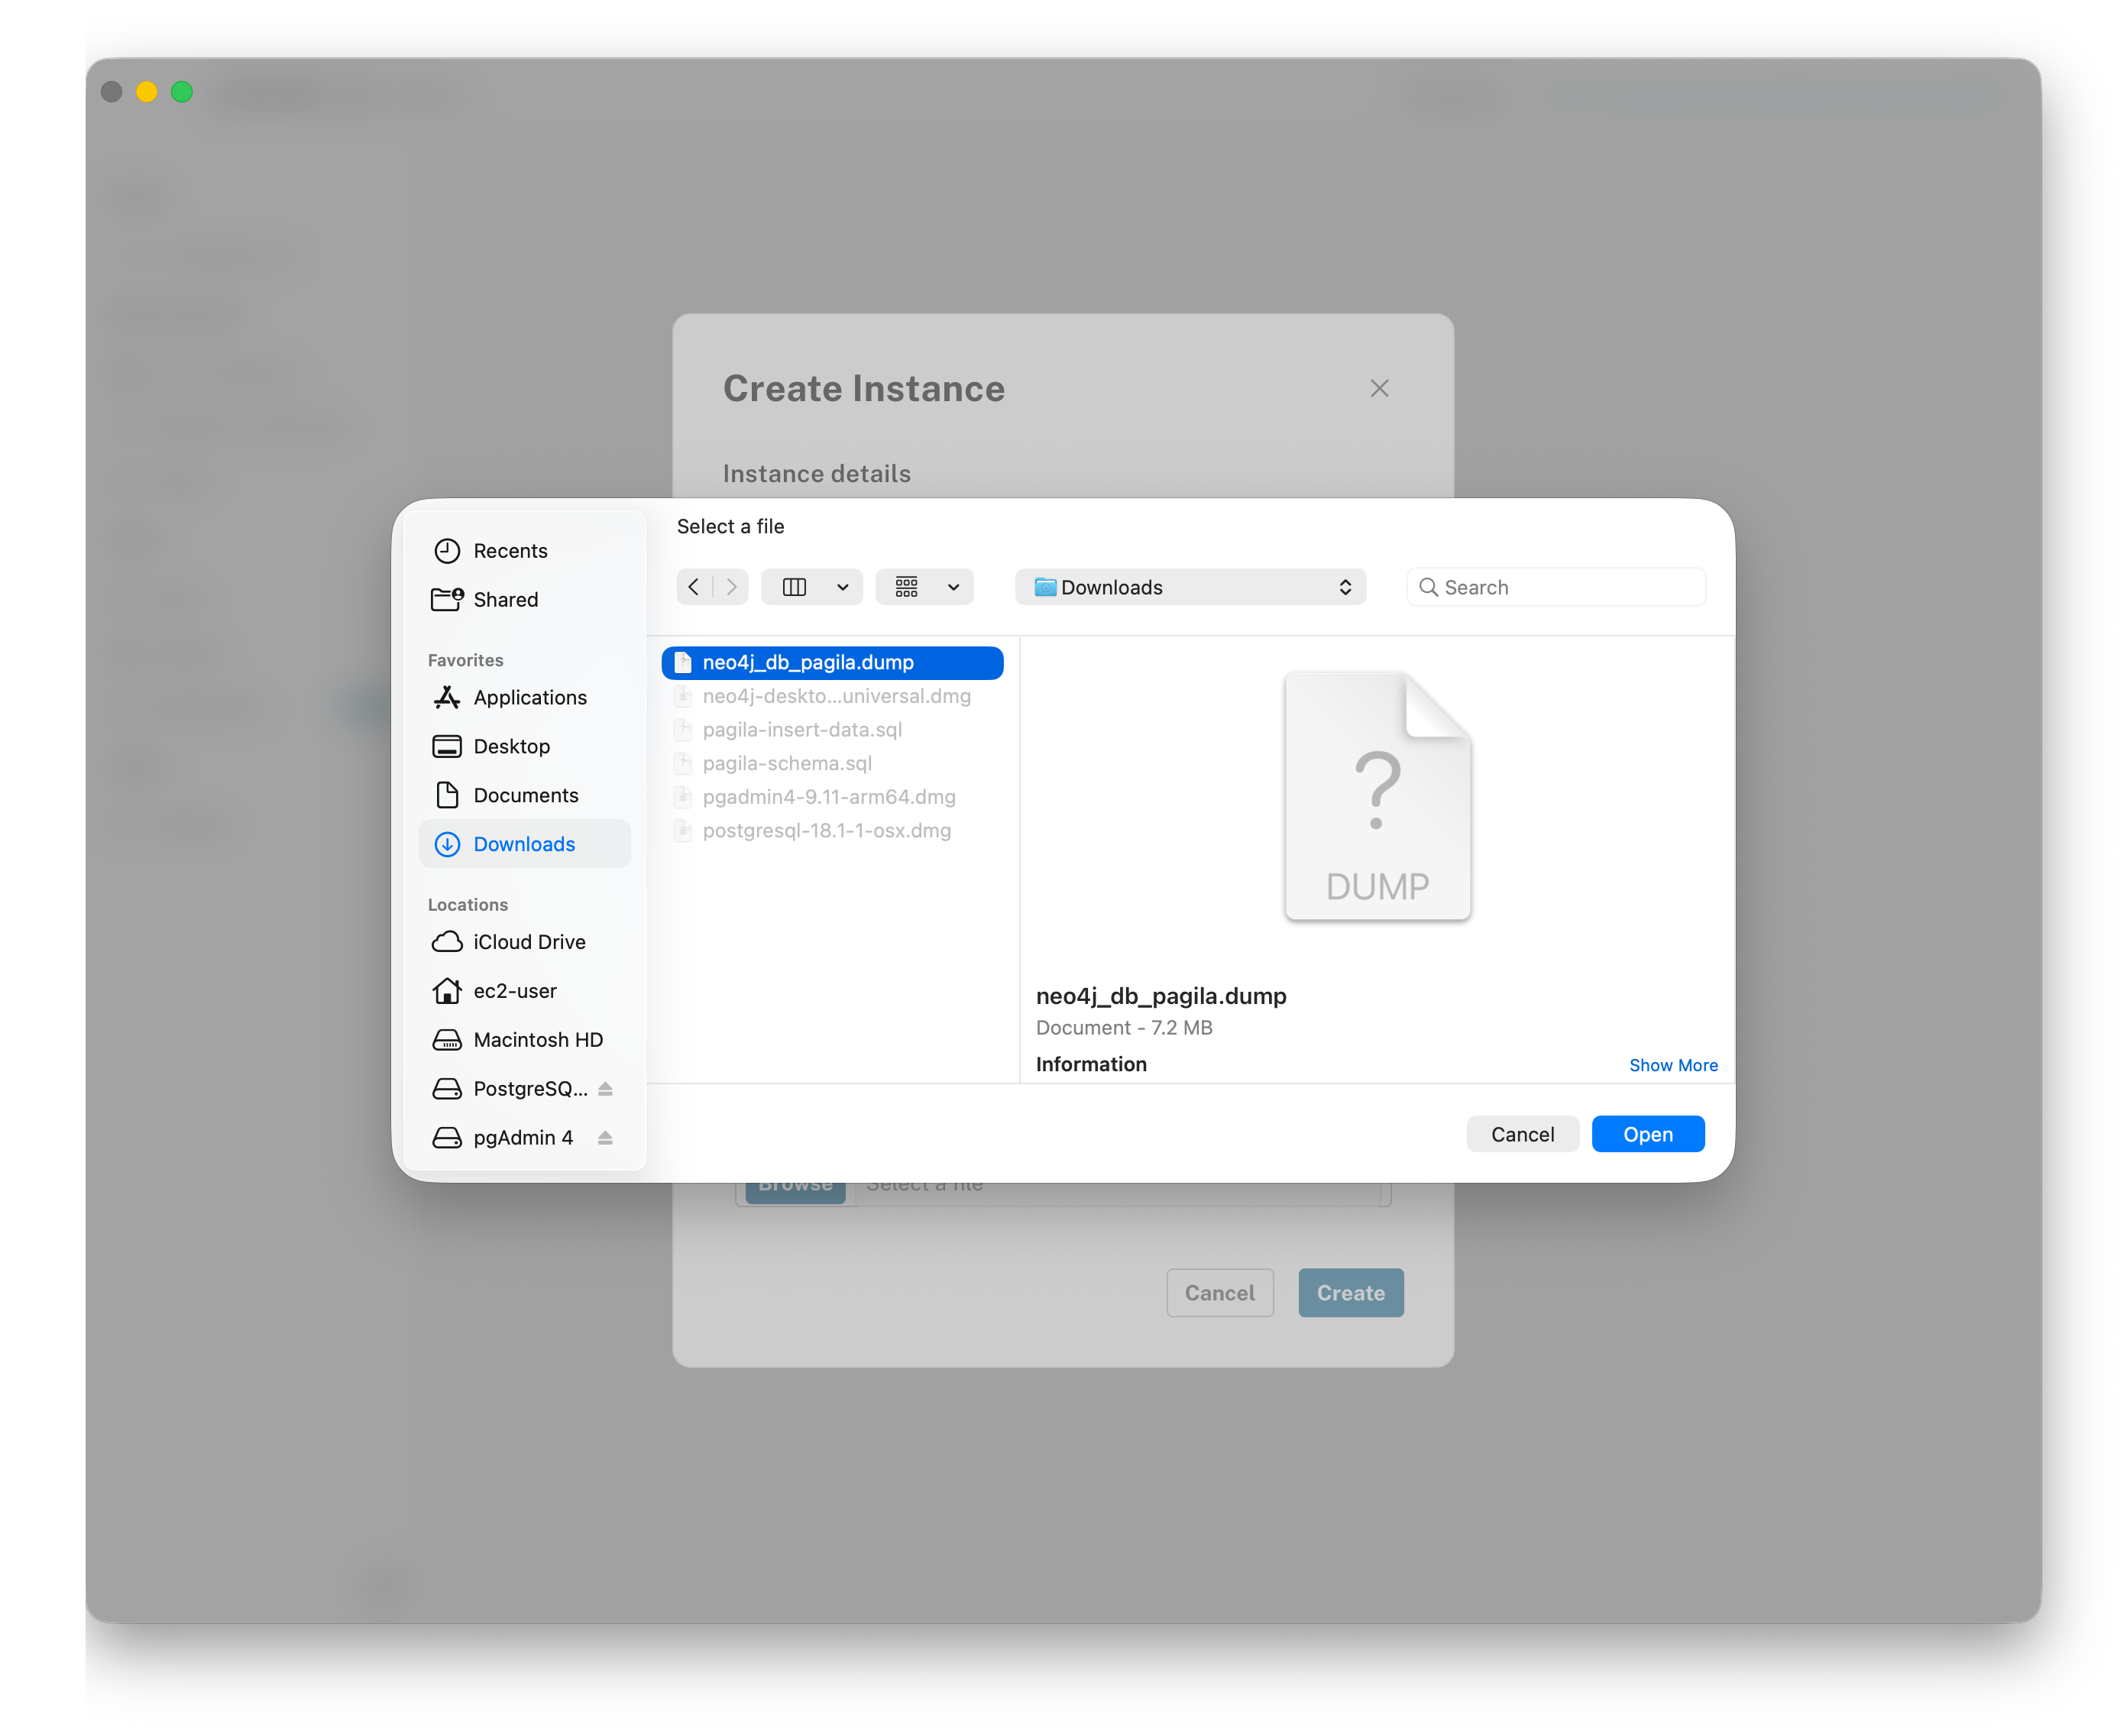
\includegraphics[width=.85\textwidth]{screen87.png}
\end{center}

\item Then, click the ''Create'' button to create the database.

\begin{center}
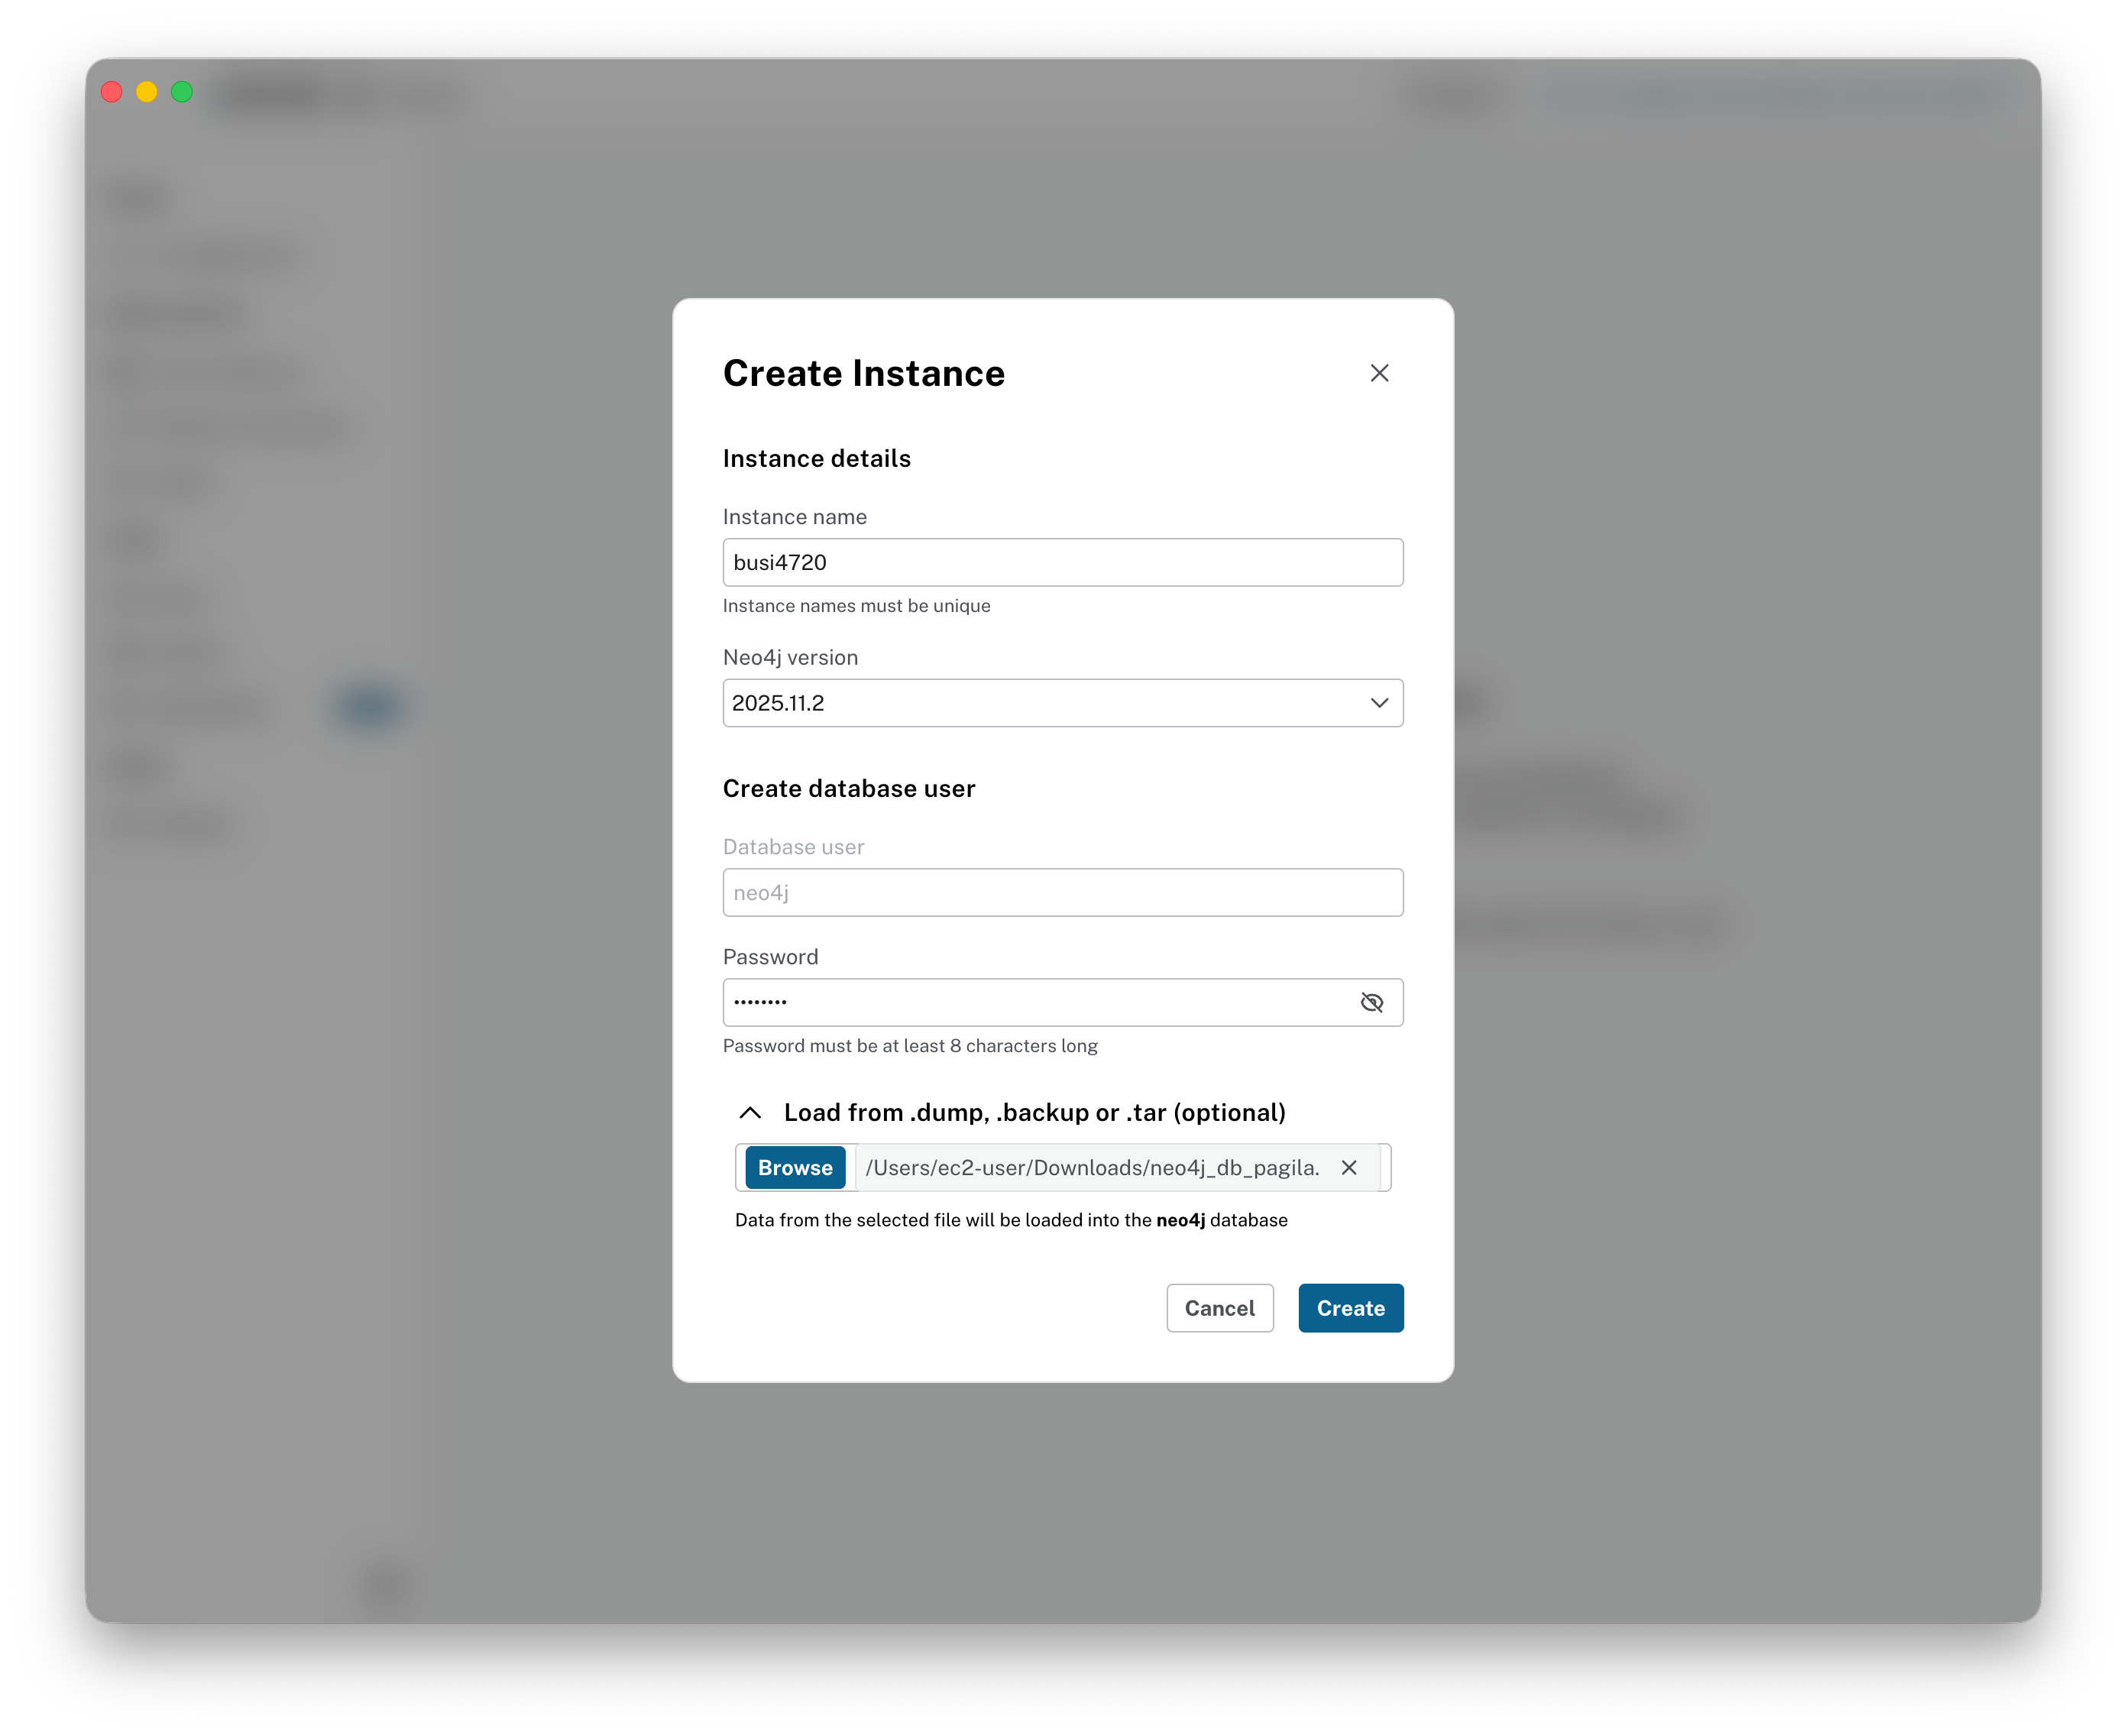
\includegraphics[width=.85\textwidth]{screen88.png}
\end{center}

\clearpage
\item Neo4J will create a new database and install the Pagila data into it. This may take a few minutes.

\begin{center}
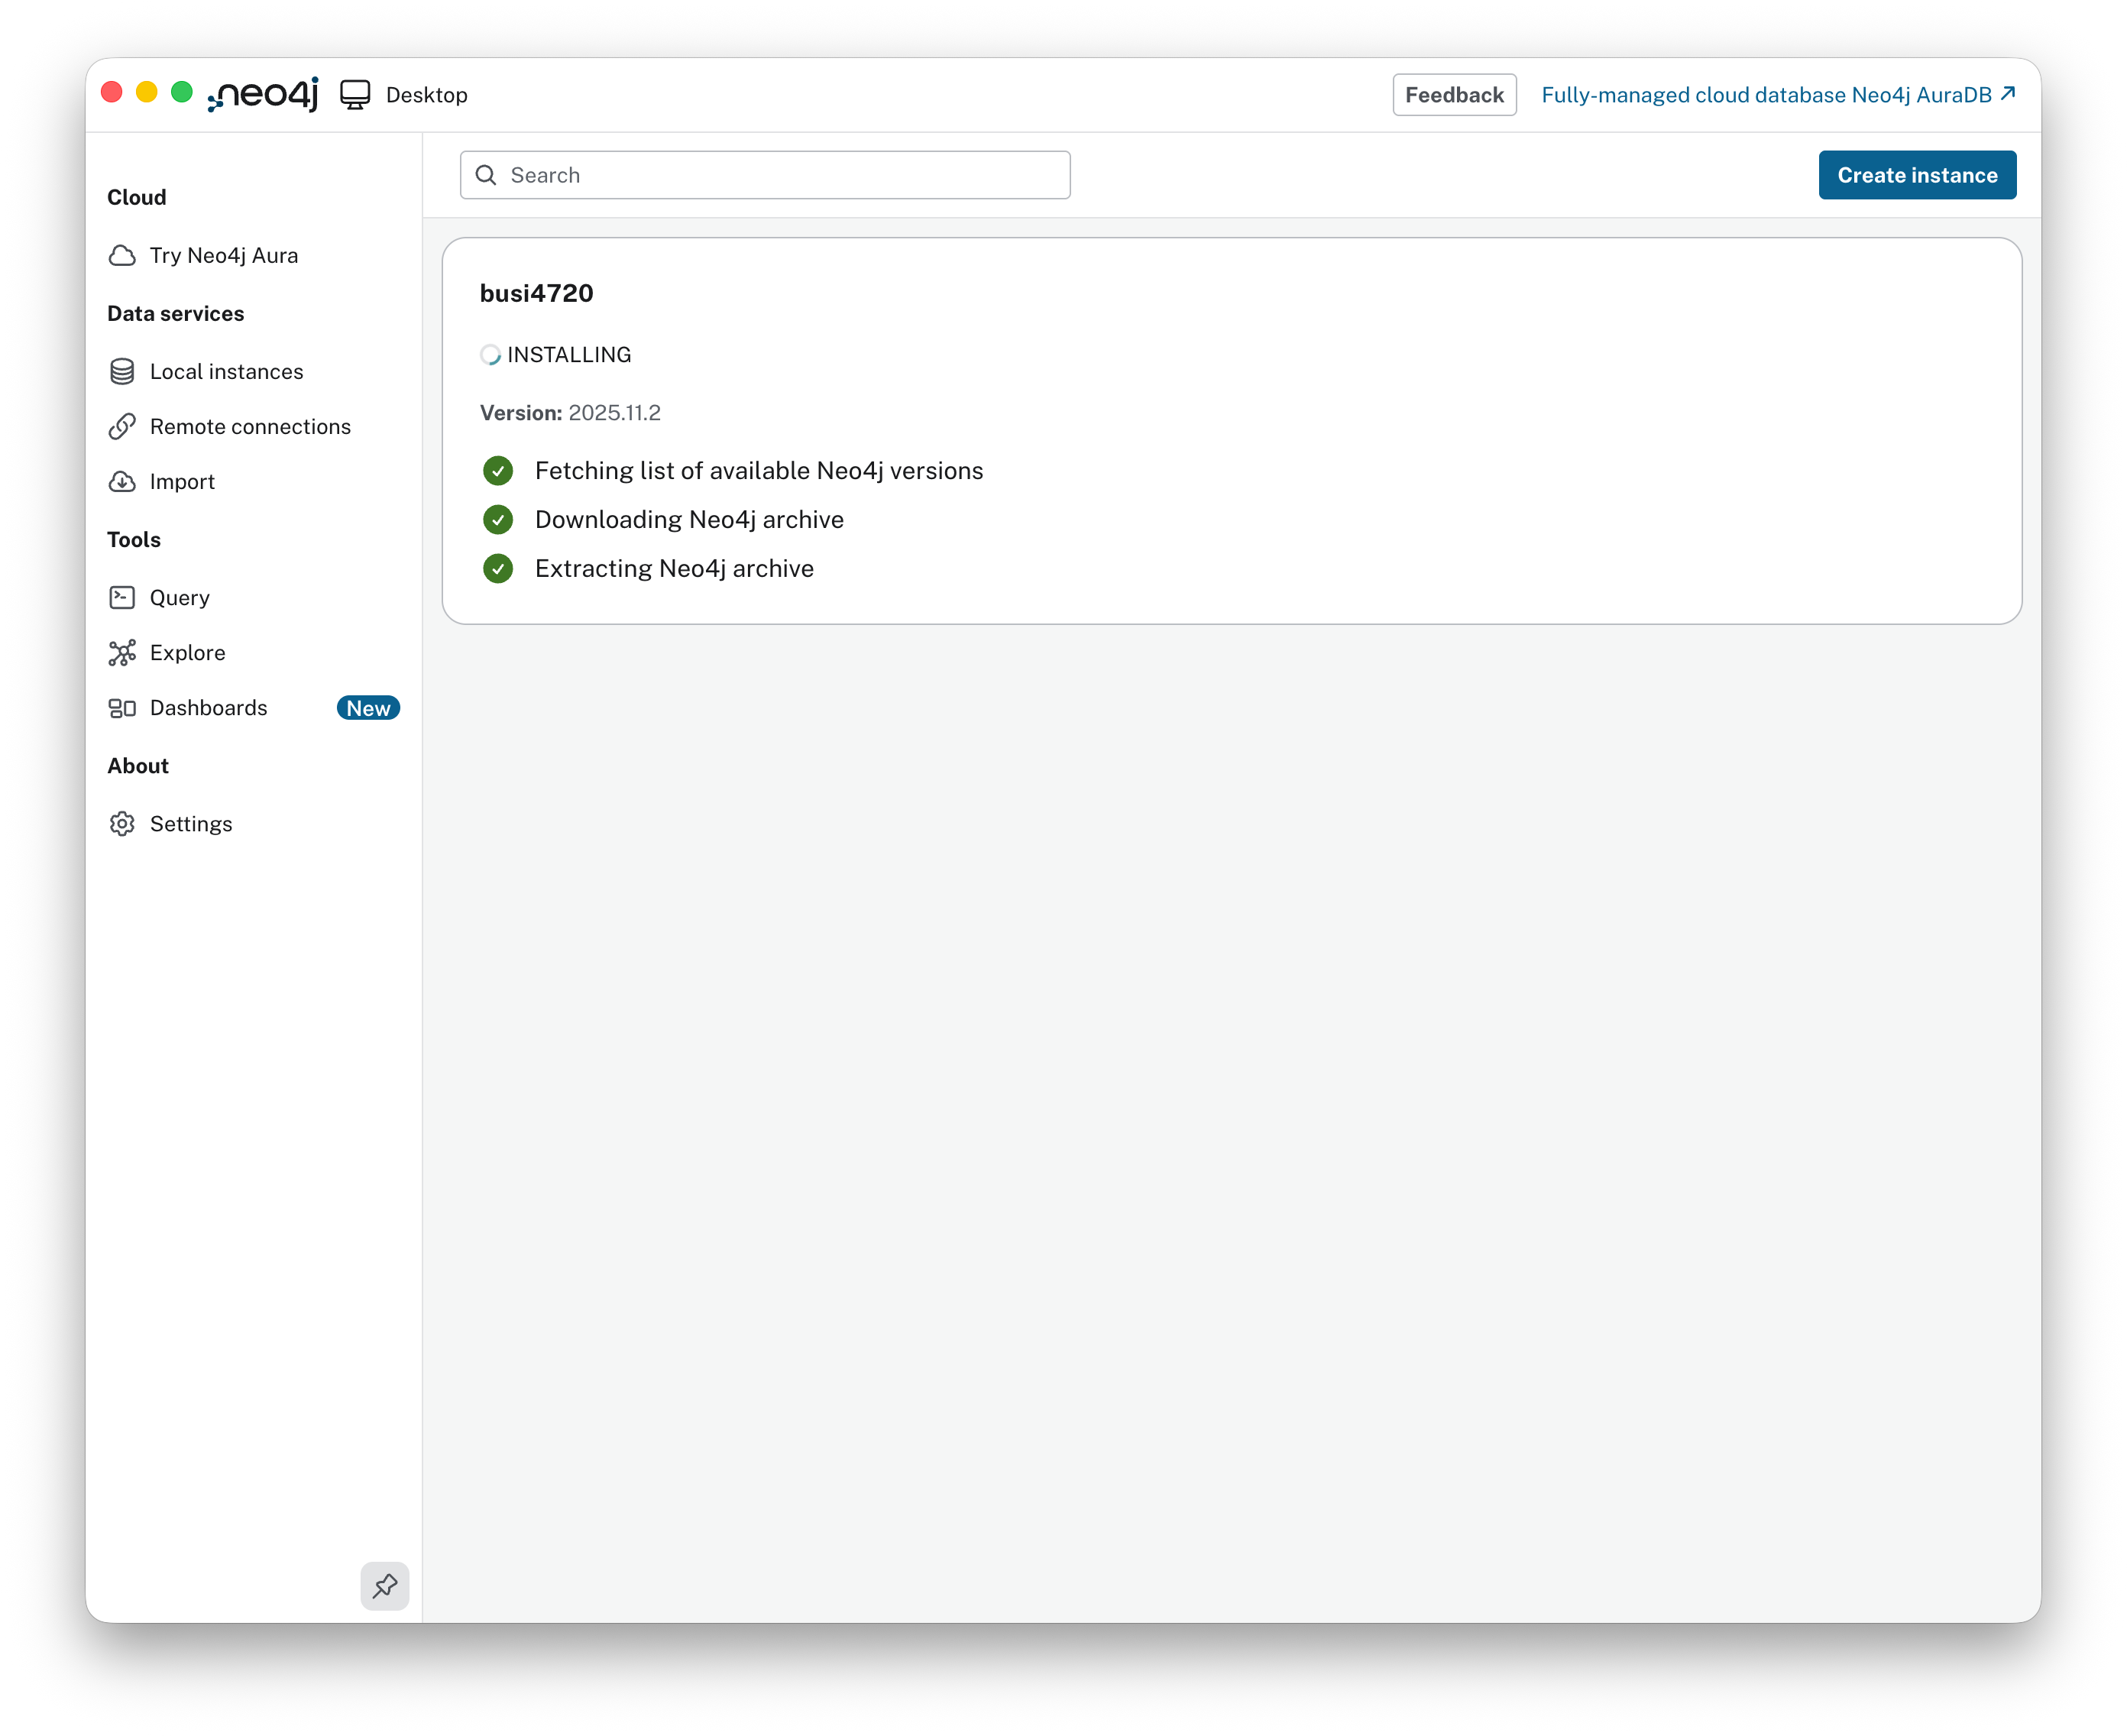
\includegraphics[width=.85\textwidth]{screen89.png}
\end{center}

\item Once the database is created, click the ''Connect'' button to connect to it in query mode.

\begin{center}
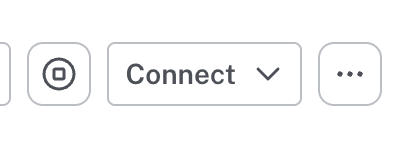
\includegraphics[width=.35\textwidth]{screen90.png}
\end{center}

\clearpage
\item The Neo4J desktop application will read the database contents, prepare a summary of nodes and relationships, and will present a query window.

\begin{center}
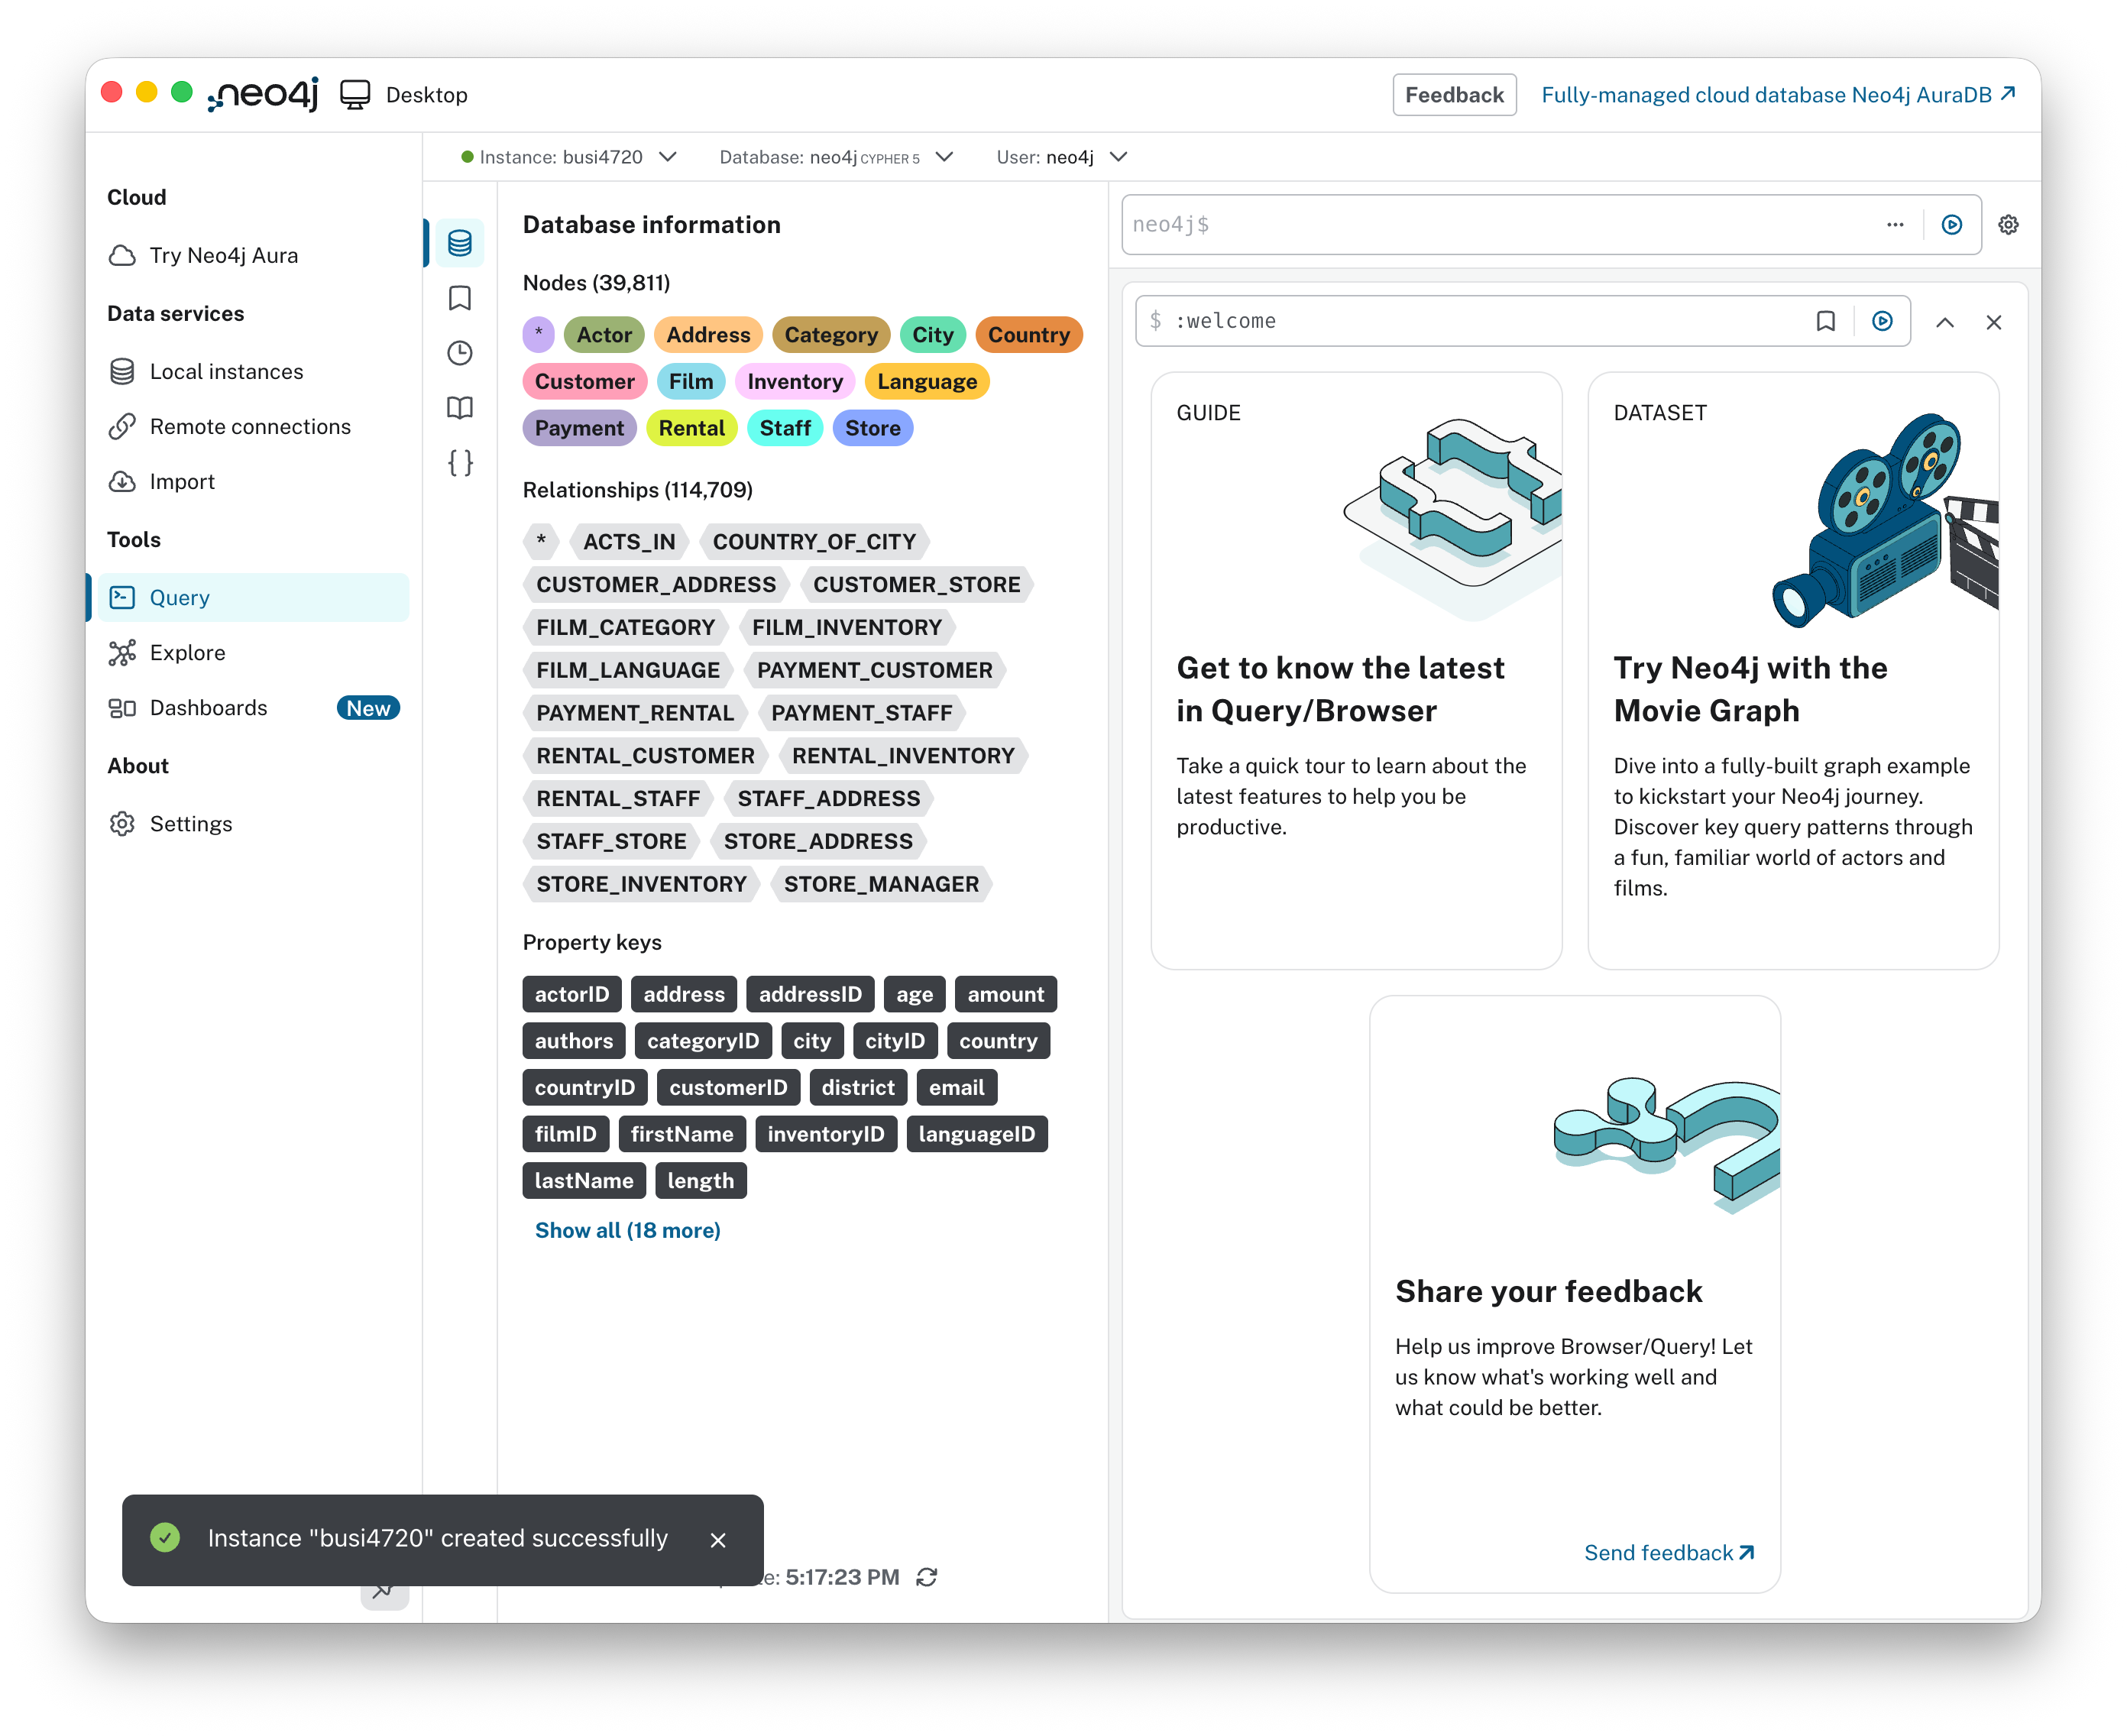
\includegraphics[width=.95\textwidth]{screen91.png}
\end{center}

\begin{infobox}
When starting the Neo4J application again, it is possible that the local database instance is not running. In this case, click the ''Start Instance'' button before connecting to the database.

\begin{center}
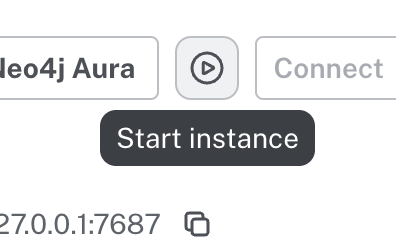
\includegraphics[width=.35\textwidth]{screen92.png}
\end{center}
\end{infobox}

\end{itemize}

